\section{Auswertung}
\label{sec:Auswertung}

Die Graphen werden sowohl mit Matplotlib \cite{matplotlib} als auch NumPy \cite{numpy} erstellt. Die Fehlerrechnung wird mithilfe von Uncertainties \cite{uncertainties} durchgeführt.

\subsection{Modellierung: Teilchen im Potentialtopf}

In Abbildung \ref{fig:Uebersicht} ist das Übersichtsspektrum für eine $\SI{600}{\milli\meter}$-Röhre und in Abbildung \ref{fig:150} das einer $\SI{150}{\milli\meter}$-Röhre zu sehen.
Eine zweite Messung des Spektrums letzterer, liefert abgesehen von geringen Abweichungen in der Amplitude dasselbe Spektrum.
Beispielhaft sind die Parameter des 1. Peaks der beiden Messungen in Tabelle \ref{tab:param} zu sehen.

\begin{figure}
\centering
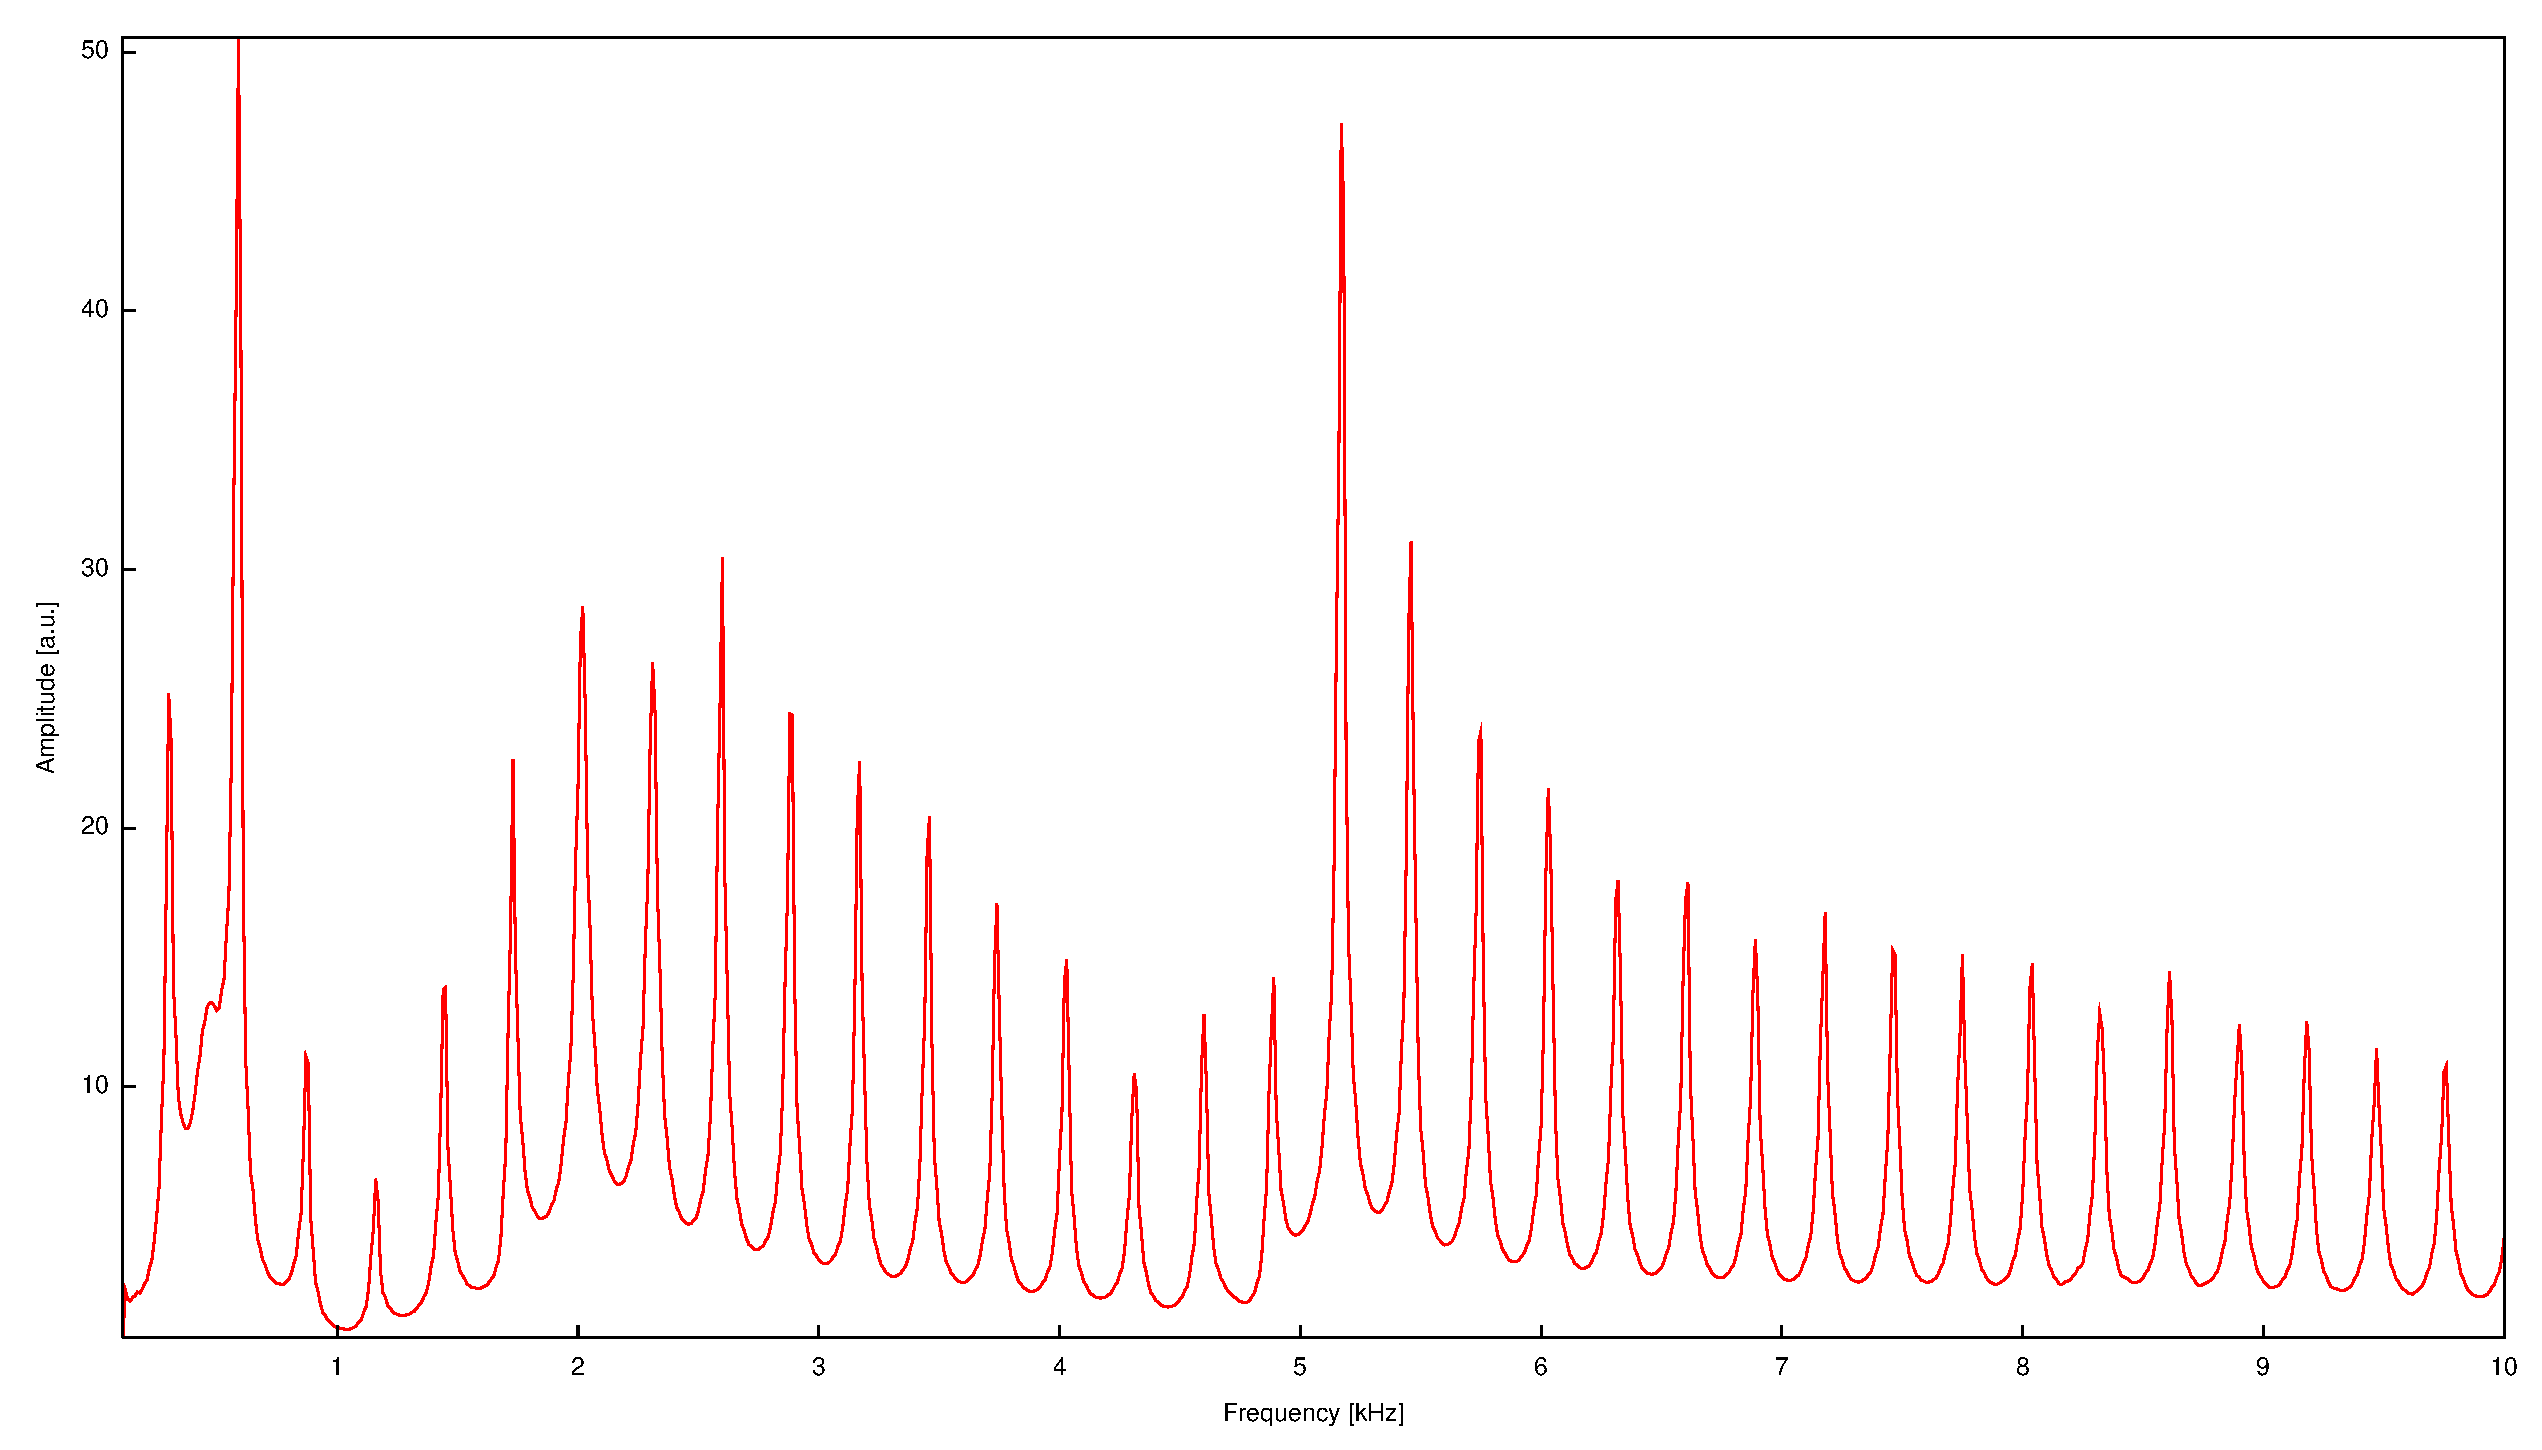
\includegraphics[width=\linewidth-60pt,height=\textheight-60pt,keepaspectratio]{FP-V23data/1.1_600mm.eps}
\caption{Spektrum einer $\SI{600}{\milli\meter}$-Röhre.}
\label{fig:Uebersicht}
\end{figure}
\begin{figure}
\centering
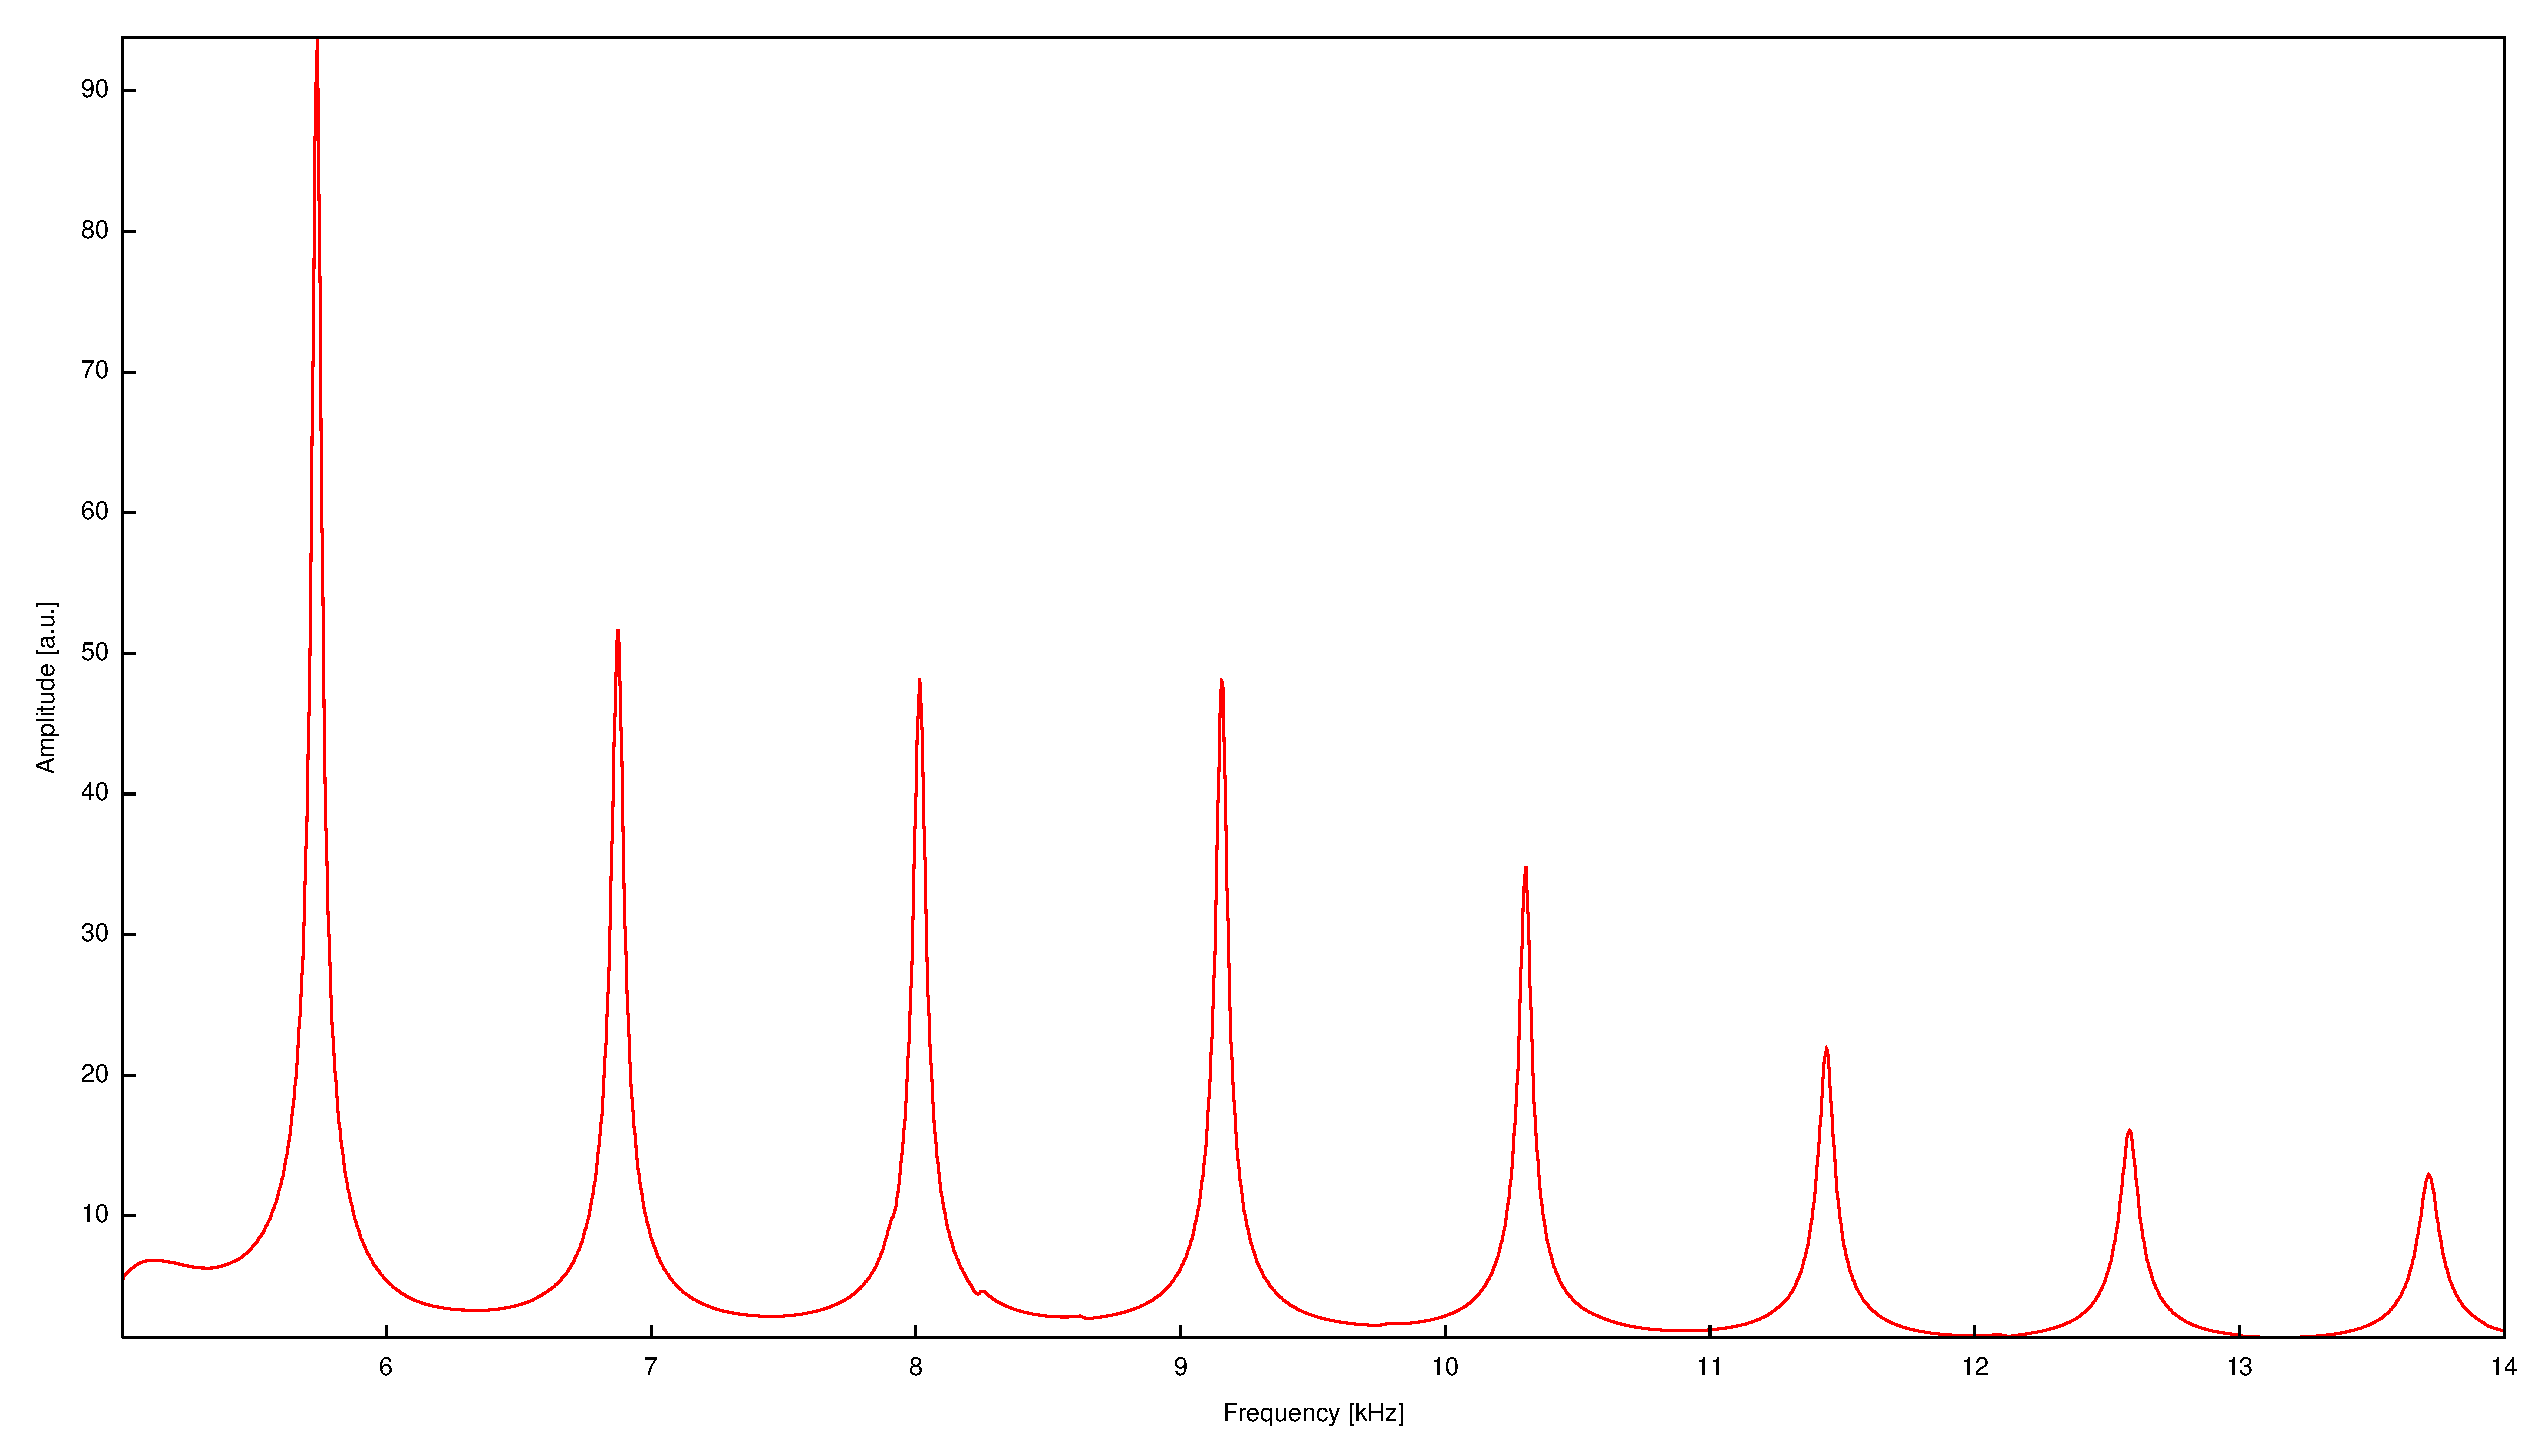
\includegraphics[width=\linewidth-60pt,height=\textheight-60pt,keepaspectratio]{FP-V23data/1.2(4.1)_150mm.eps}
\caption{Spektrum einer $\SI{150}{\milli\meter}$-Röhre.}
\label{fig:150}
\end{figure}
\begin{table}
\caption{Parameter des 1. Peaks von zwei spektralen Analysen einer $\SI{600}{\milli\meter}$ langen Röhre.}
\centering
\label{tab:params}
	\sisetup{table-format=1.2}
	\begin{tabular}{S[table-format=1.0]S[table-format=4.3]S[table-format=2.4]}
		\toprule
		{Messung} & {$f_\text{1}/(\si{\hertz})$} & {$A_\text{1}/(\si{a\text{.}u\text{.}})$} \\
		\midrule
		 1 & 5747.706 & 92.8953 \\
		 2 & 5747.706 & 92.0576 \\
		\bottomrule
	\end{tabular}

\end{table}

\subsection{Modellierung: Das Wasserstoffatom}

In Abbildung \ref{fig:Overview} sind das Spektrum des sphärischen Resonators bei $\alpha=\SI{0}{\degree}$ und $\alpha=\SI{180}{\degree}$
zu sehen.
Die Resonanzfrequenzen $f_.n$ verändern sich nicht, jedoch fällt auf, dass bei $\alpha=\SI{0}{\degree}$ die Amplitude des 2. Peaks das Spektrum dominiert, während bei $\alpha=\SI{180}{\degree}$ alle Peaks in etwa dieselbe Höhe haben. Außerdem zeigt sich, dass in diesem Spektrum alle Peaks eine größere Amplitude aufweisen, als bei $\alpha=\SI{0}{\degree}$.\\
In Abbildung \ref{fig:5k_Peak1} und \ref{fig:5k_Peak2} ist für $\alpha=\SI{0}{\degree}$ und für $\alpha=\SI{40}{\degree}$, der Peak bei $f\approx\SI{5000}{\hertz}$ näher aufgelöst.
Es zeigt sich das der Hauptpeak mit zunehmendem $\alpha$ leicht zunimmt. Bei $\alpha=\SI{40}{\degree}$ bildet sich ein stark zunehmender Nebenpeak aus, der bei $\alpha=\SI{0}{\degree}$ von einer Einbuchtung überlagert wird.\\
In Abbildung \ref{fig:polar} sind die Polarplots der Peaks im Bereich von $\SI{2000}{\hertz}$ bis $\SI{7000}{\hertz}$ zu sehen.
Der Vergleich mit Bildern aus der Literatur\cite{V23}, liefert den Zusammenhang zwischen den ersten vier Peaks und den Kugelflächenfunktionen:
\begin{align*}
.{Peak 1}&\mathop{\widehat{=}} Y^0_1\\
.{Peak 2}&\mathop{\widehat{=}} Y^0_2\\
.{Peak 3}&\mathop{\widehat{=}} Y^0_3\\
.{Peak 4}&\mathop{\widehat{=}} Y^0_4\\
\end{align*}
Der 5. Polarplot lässt sich keinem Zustand mit $m=0$ zuordnen und ähnelt am ehesten der Kugelflächenfunktion $Y^.1_.2$.
\begin{figure}
\centering
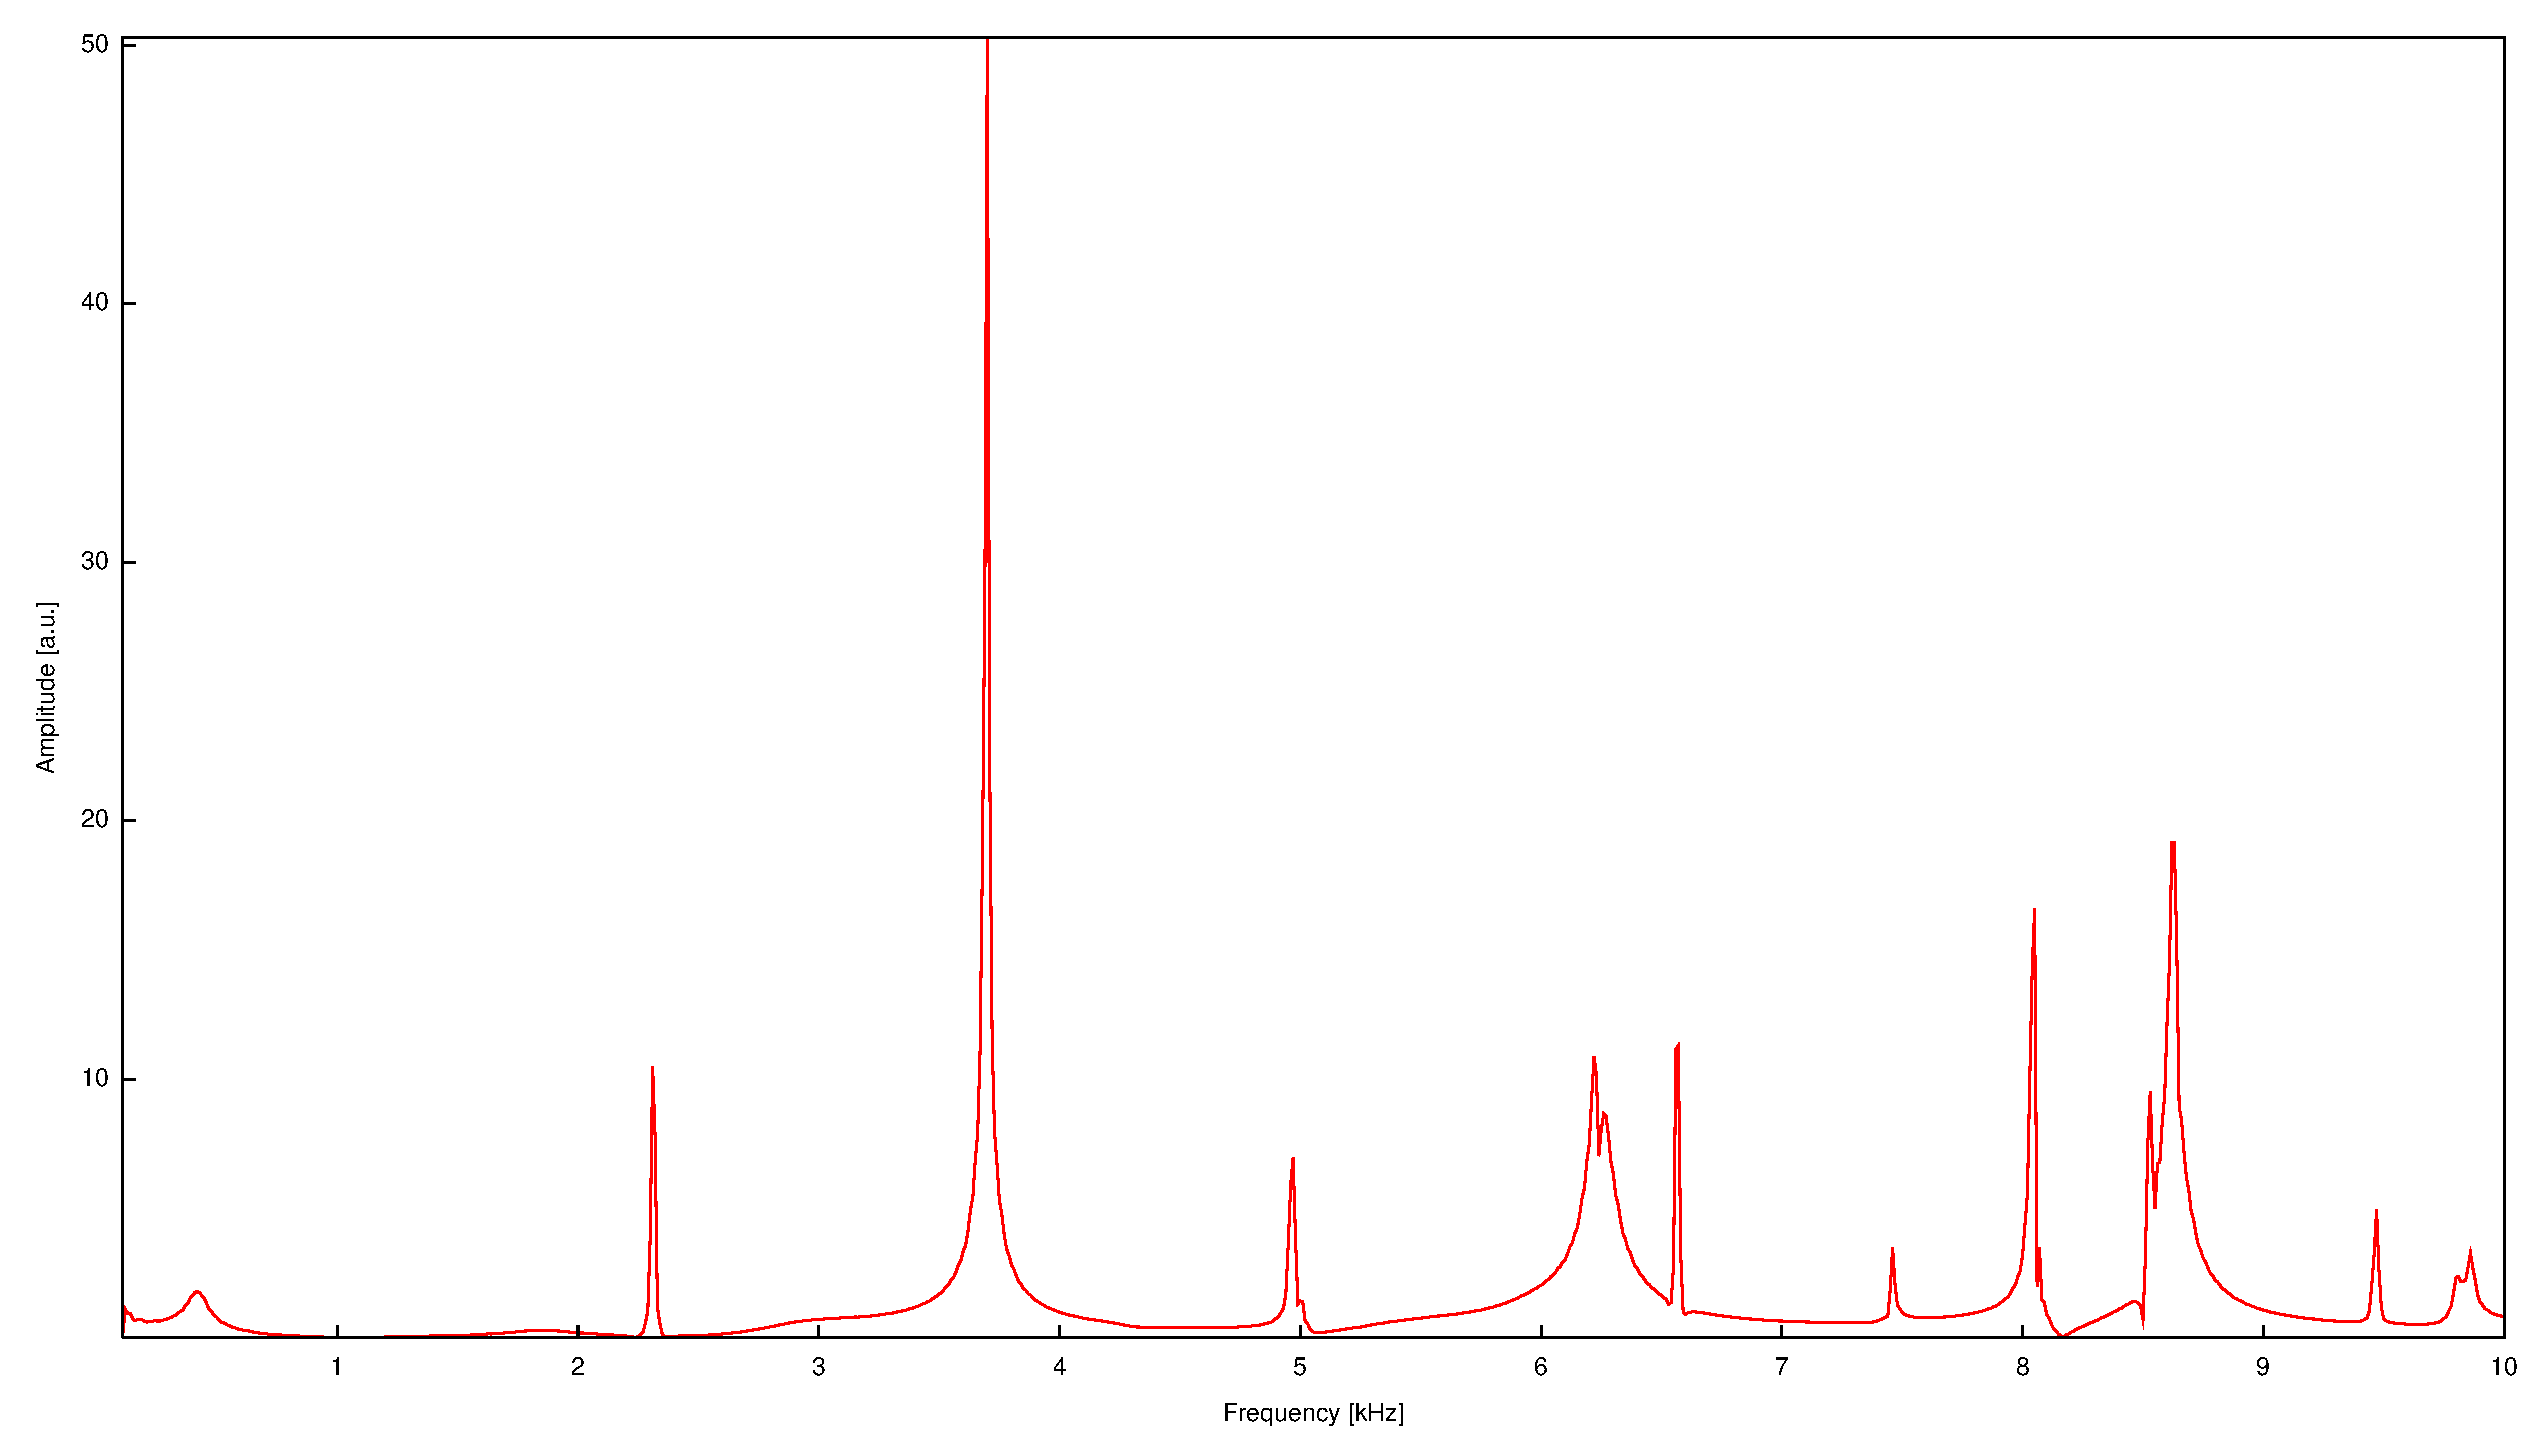
\includegraphics[width=\linewidth-60pt,height=\textheight-60pt,keepaspectratio]{FP-V23data/2.1_0degree.eps}
\caption{Spektrum im sphärischen Resonate für $\alpha=\SI{0}{\degree}$.}
\label{fig:Overview1}
\end{figure}
\begin{figure}
\centering
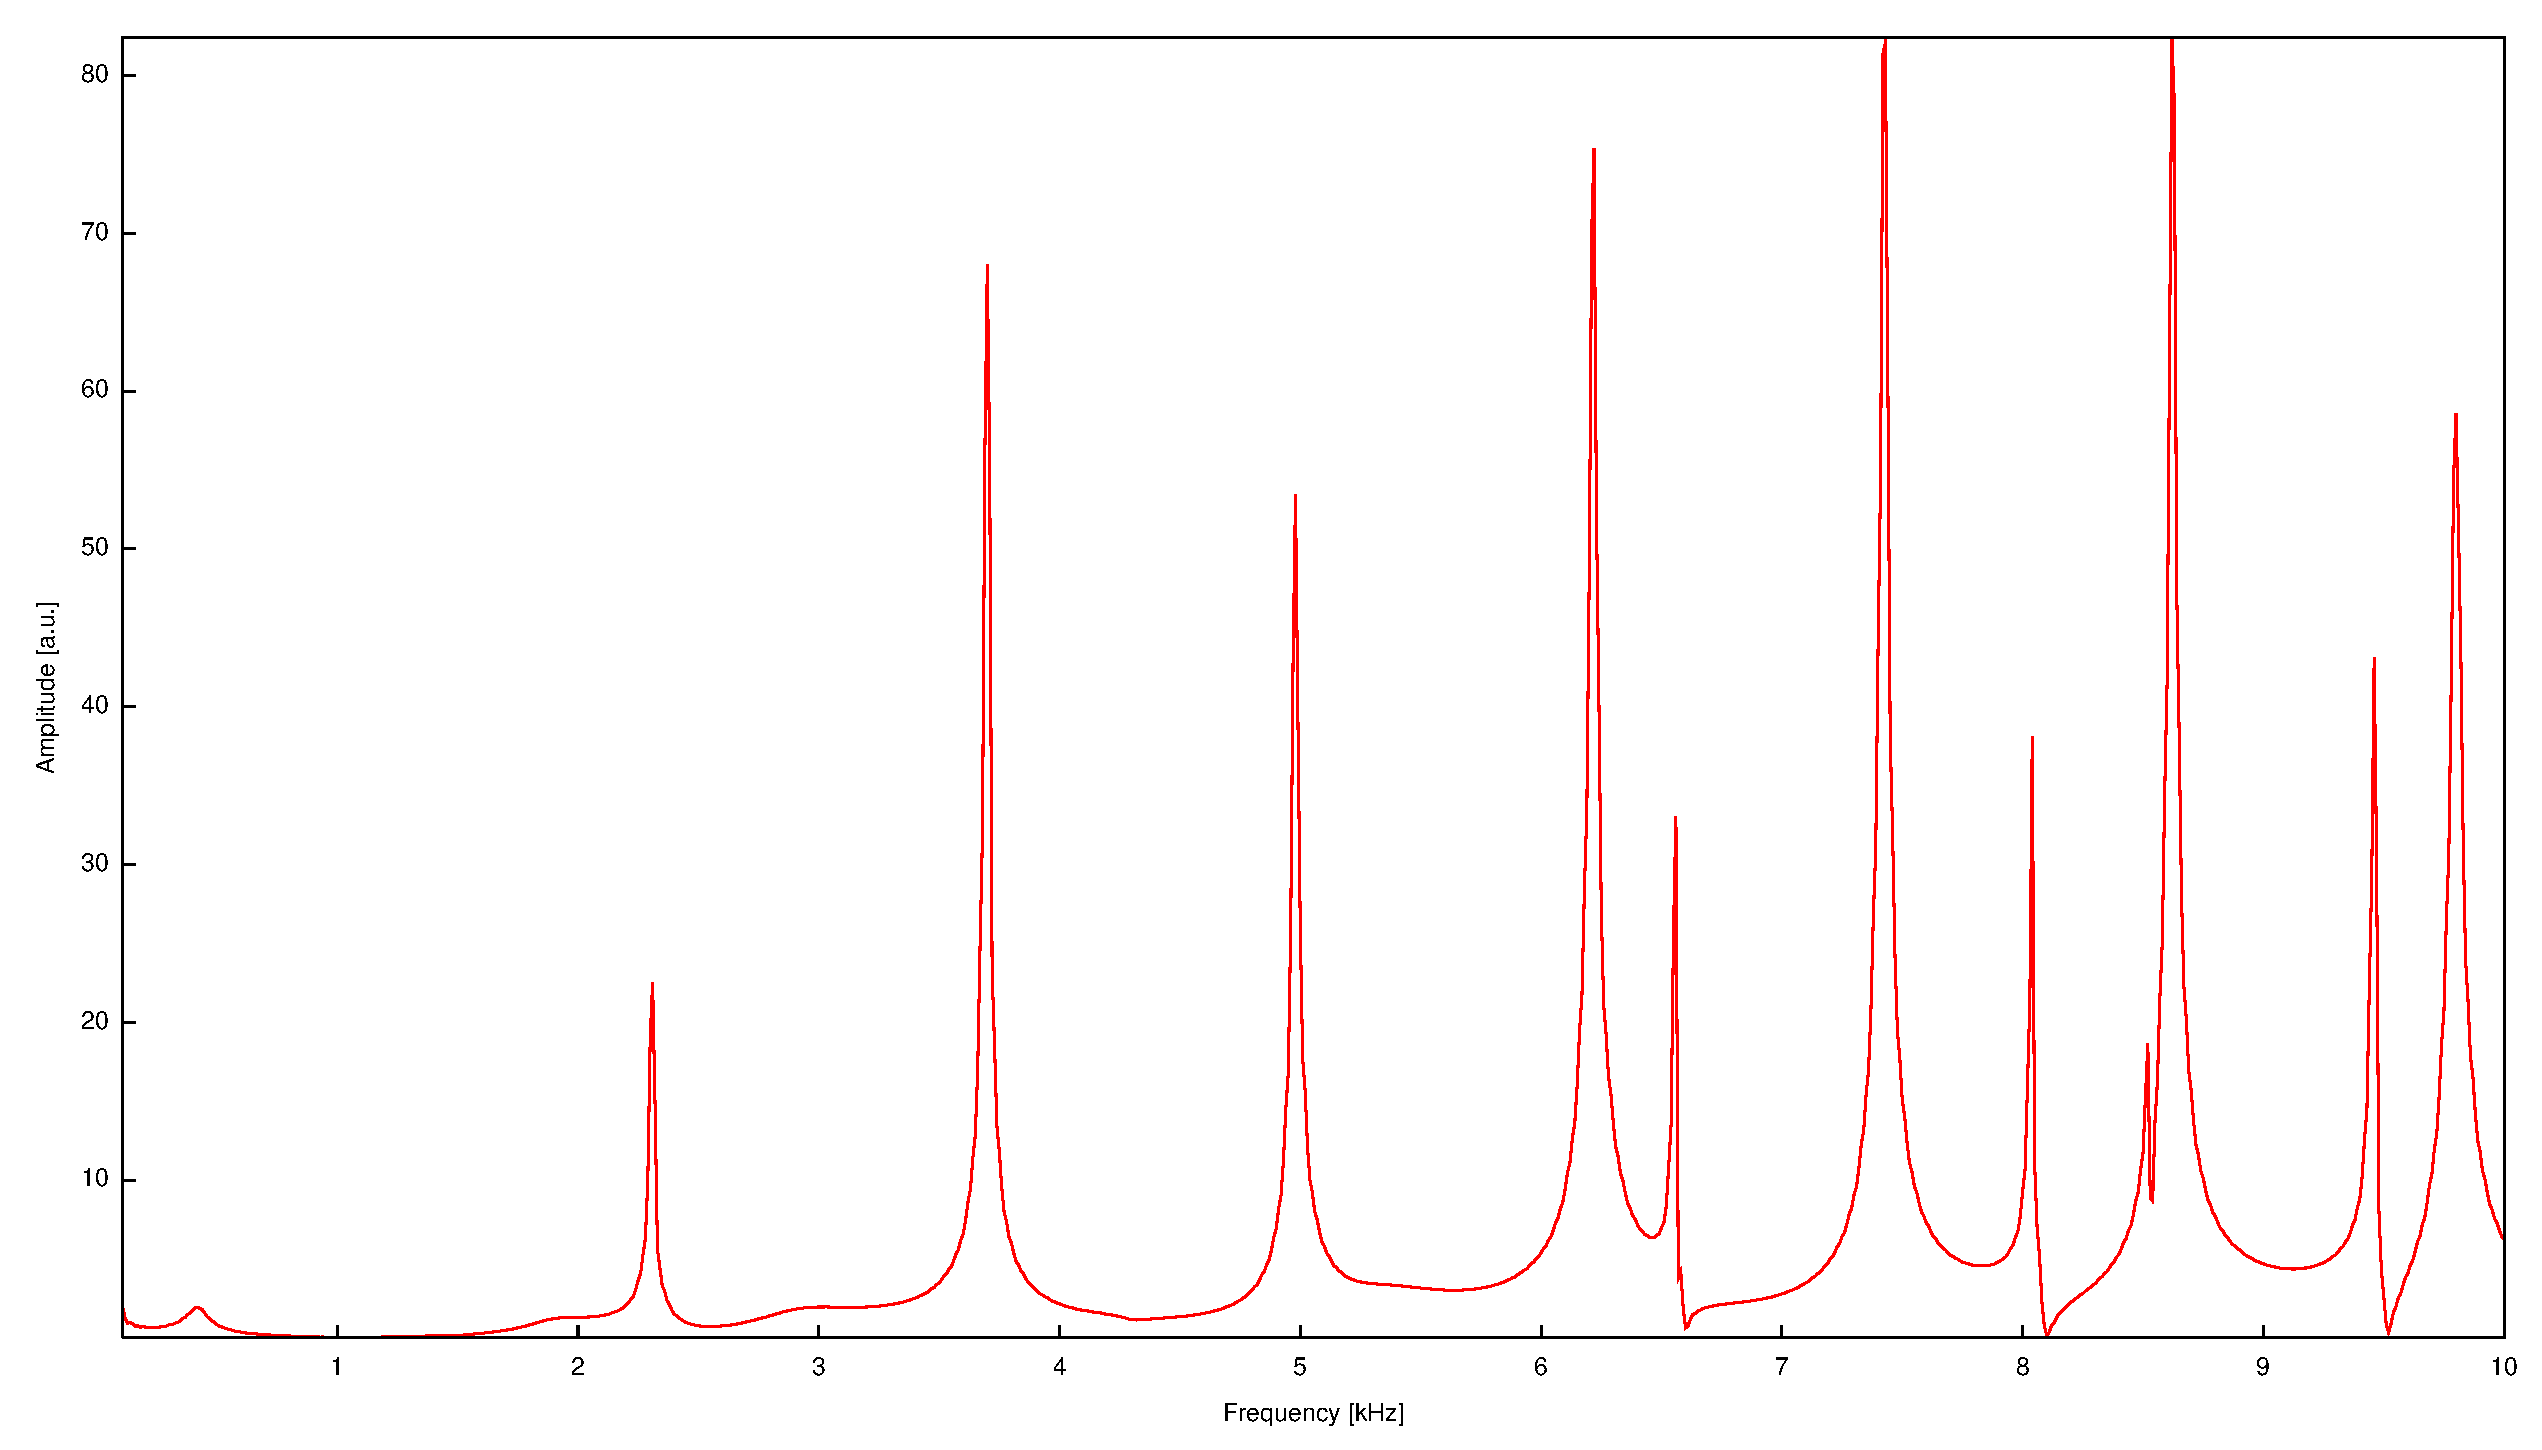
\includegraphics[width=\linewidth-60pt,height=\textheight-60pt,keepaspectratio]{FP-V23data/2.1_180degree.eps}
\caption{Spektrum im sphärischen Resonate für $\alpha=\SI{180}{\degree}$.}
\label{fig:Overview2}
\end{figure}
\begin{figure}
\centering
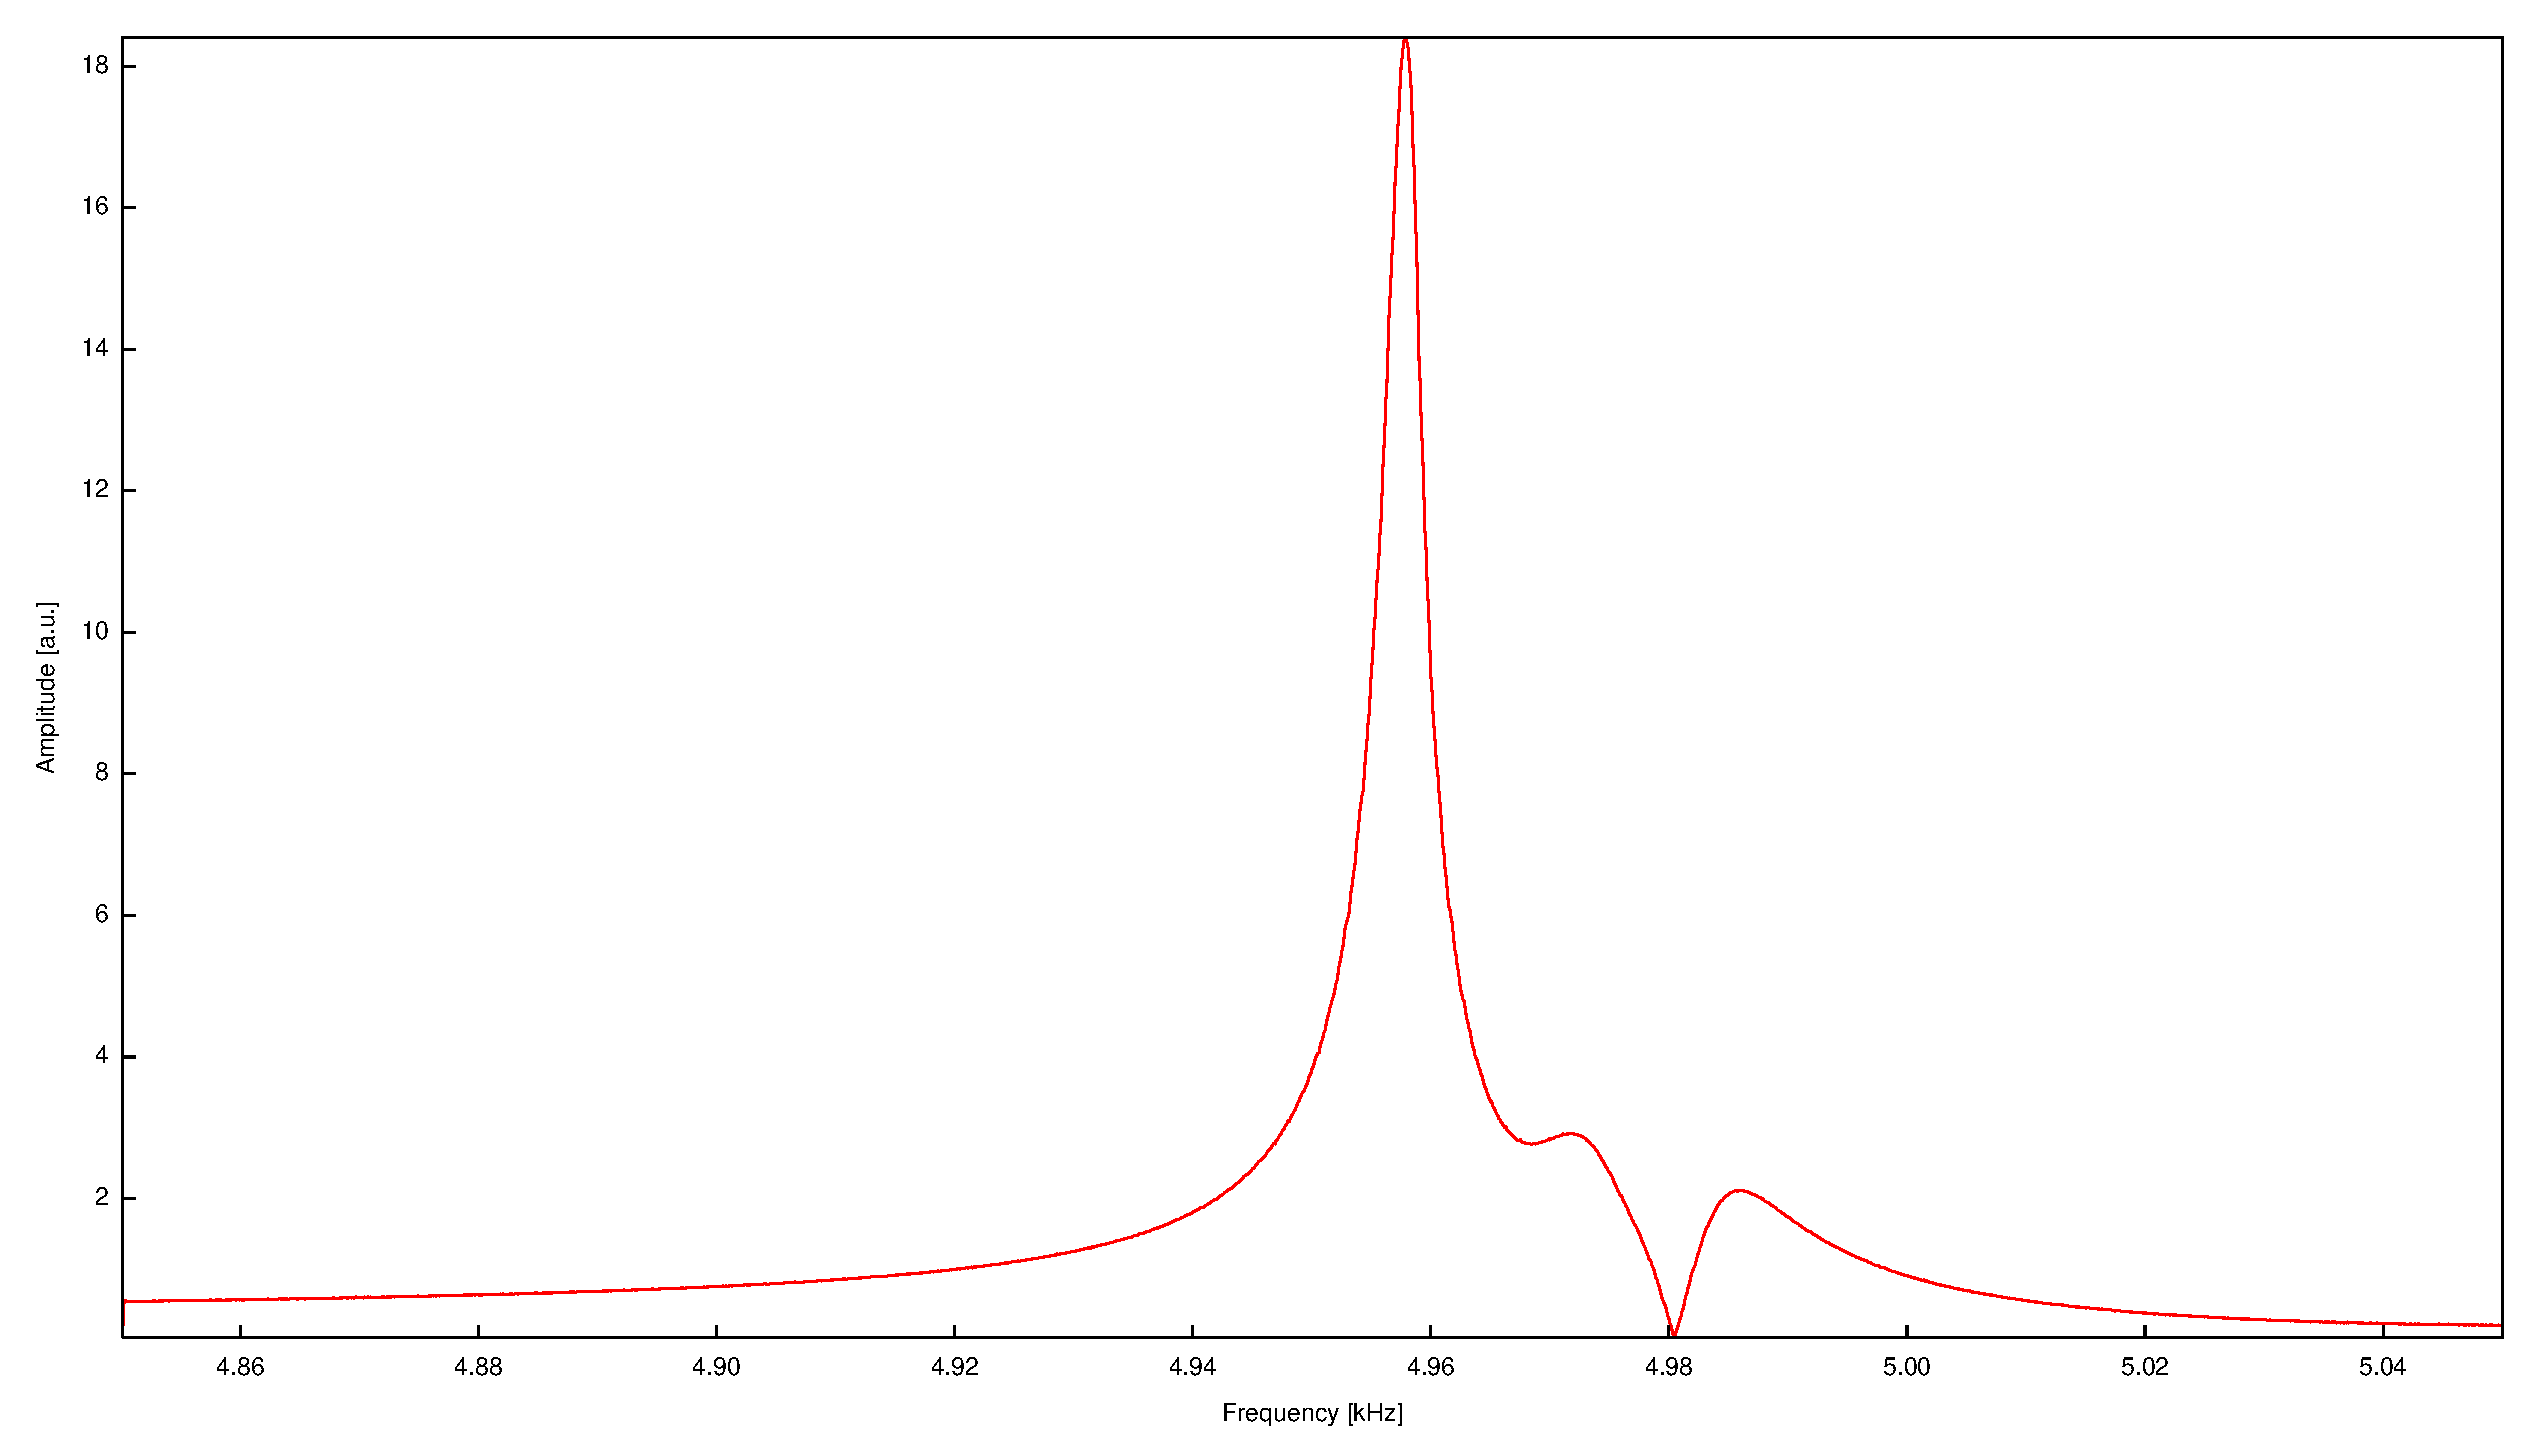
\includegraphics[width=\linewidth-60pt,height=\textheight-60pt,keepaspectratio]{FP-V23data/2.2_0degree.eps}
\caption{Nähere Aufnahme des Peaks bei $f\approx\SI{5000}{\hertz}$ für $\alpha=\SI{0}{\degree}$.}
\label{fig:5k_Peak1}
\end{figure}
\begin{figure}
\centering
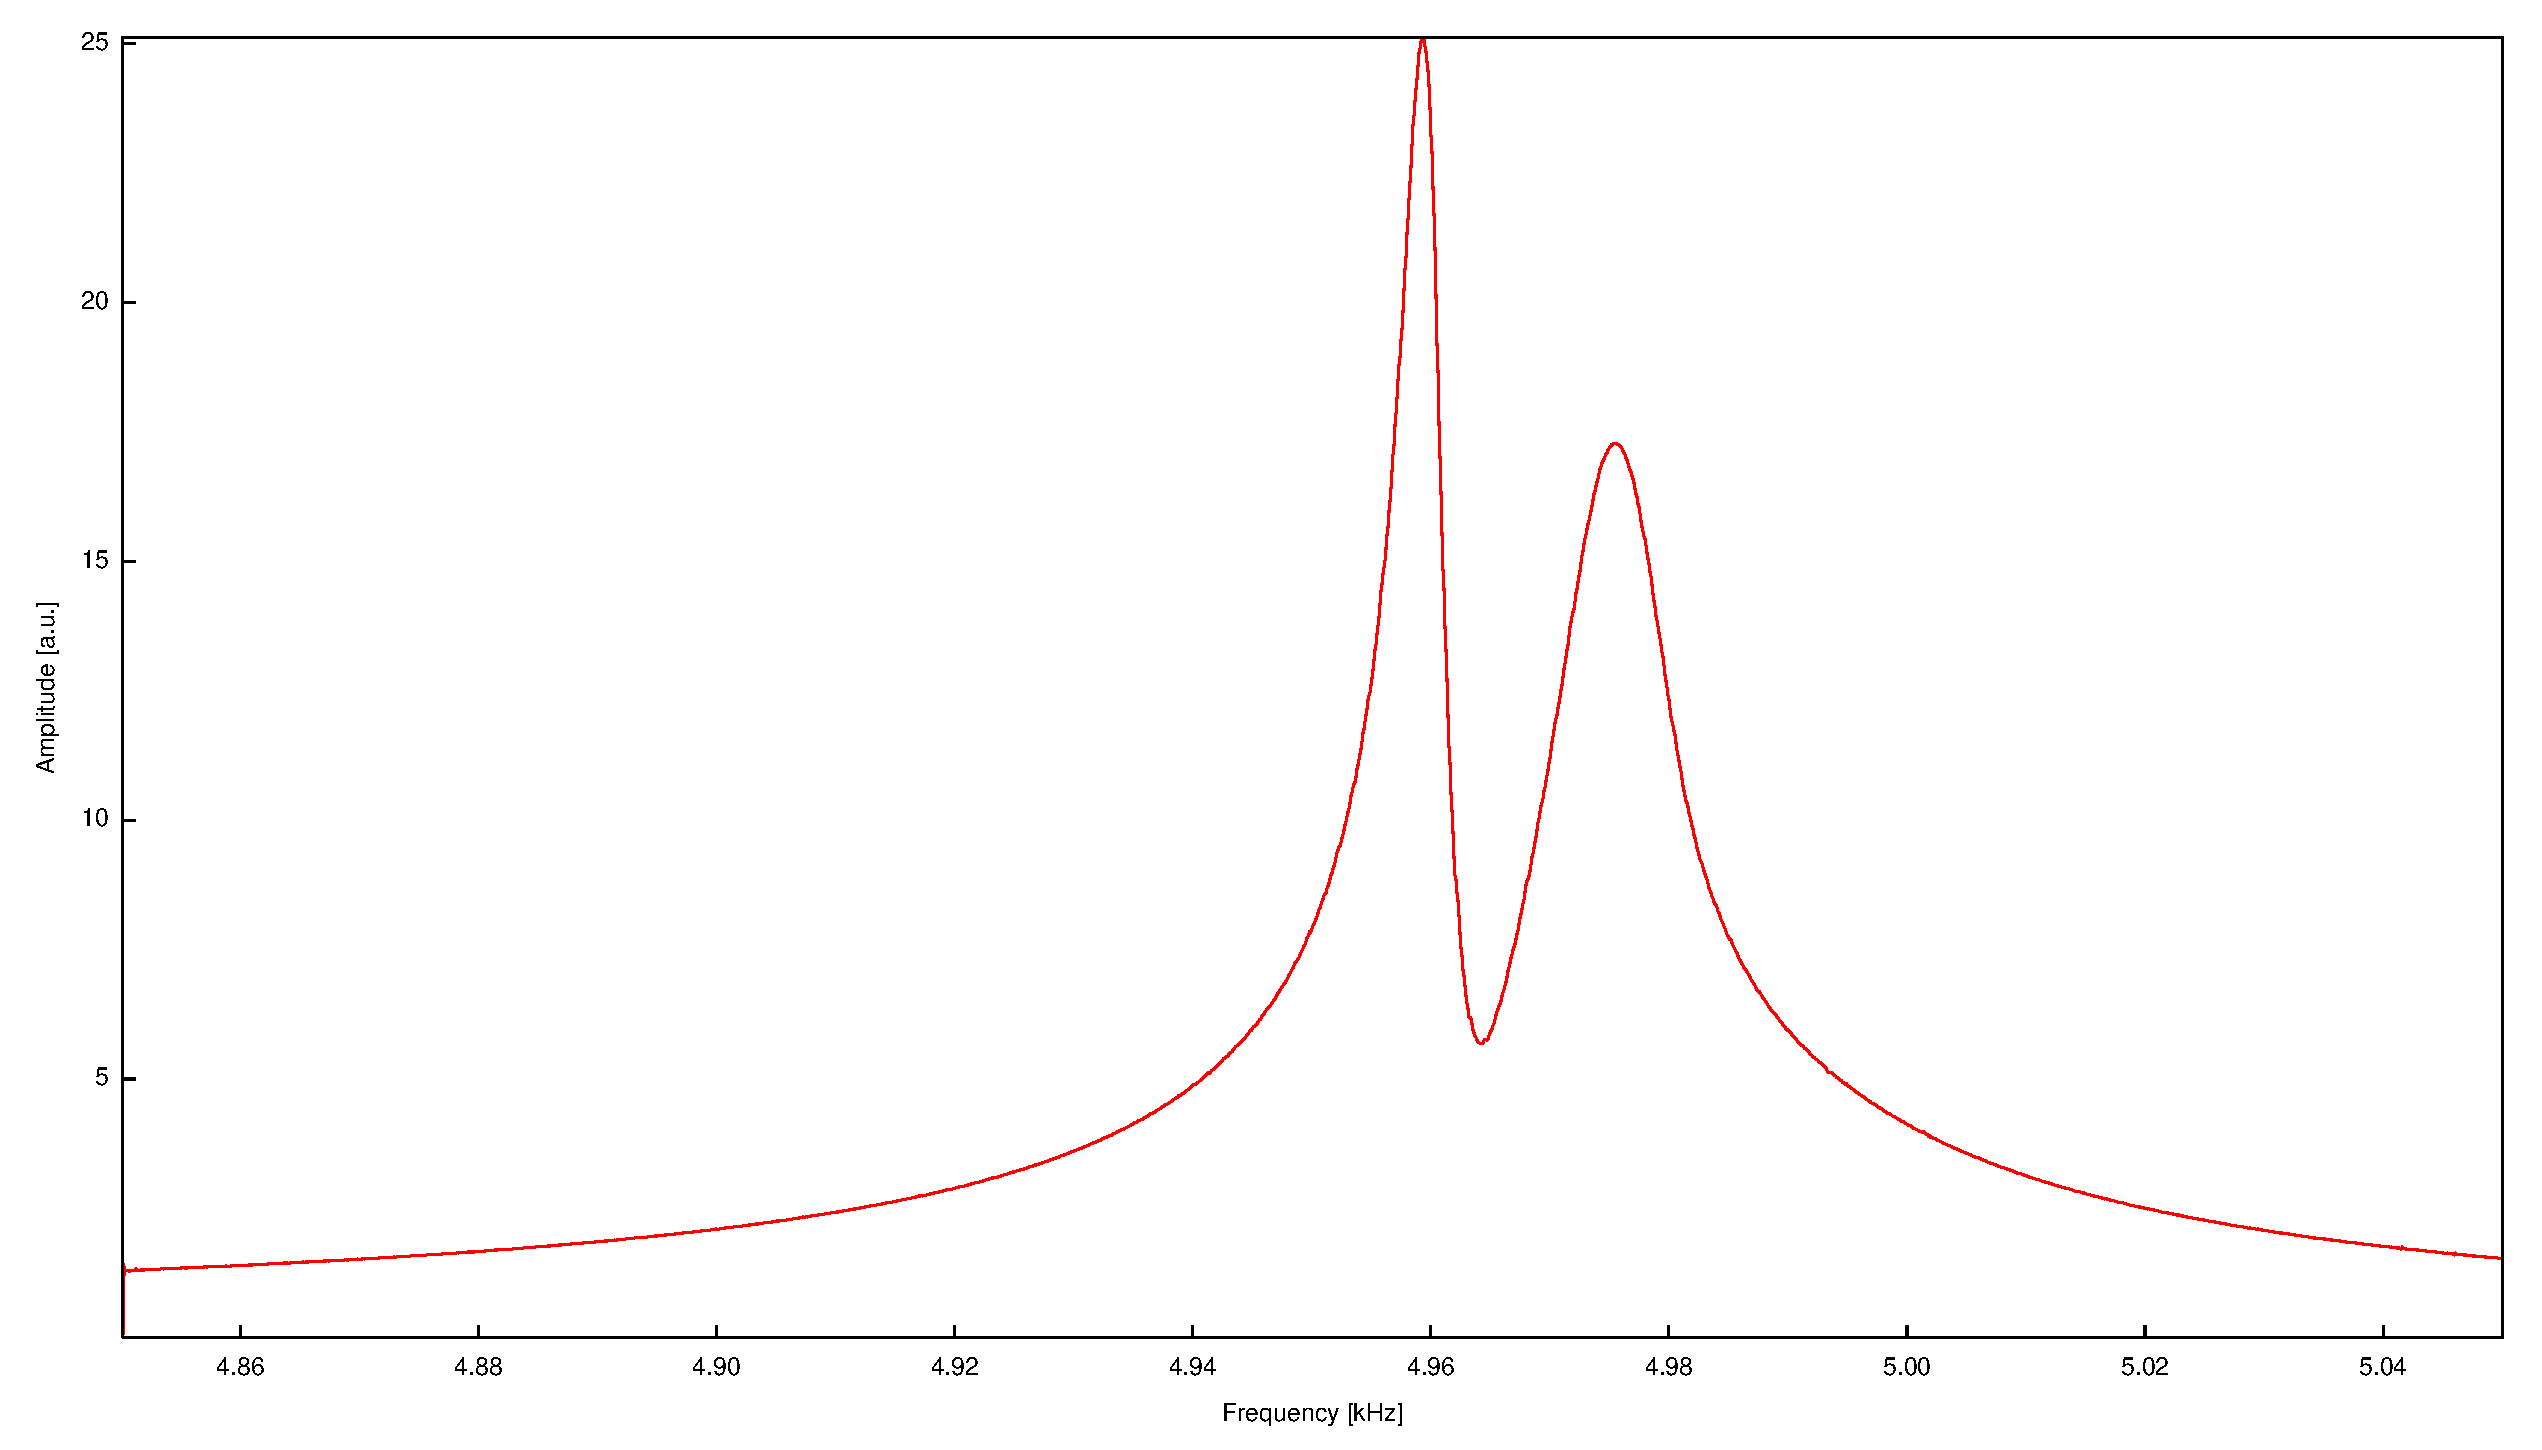
\includegraphics[width=\linewidth-60pt,height=\textheight-60pt,keepaspectratio]{FP-V23data/2.2_40degree.eps}
\caption{Nähere Aufnahme des Peaks bei $f\approx\SI{5000}{\hertz}$ für $\alpha=\SI{40}{\degree}$.}
\label{fig:5k_Peak2}
\end{figure}
\begin{figure}
\centering
\begin{minipage}{0.45\textwidth}
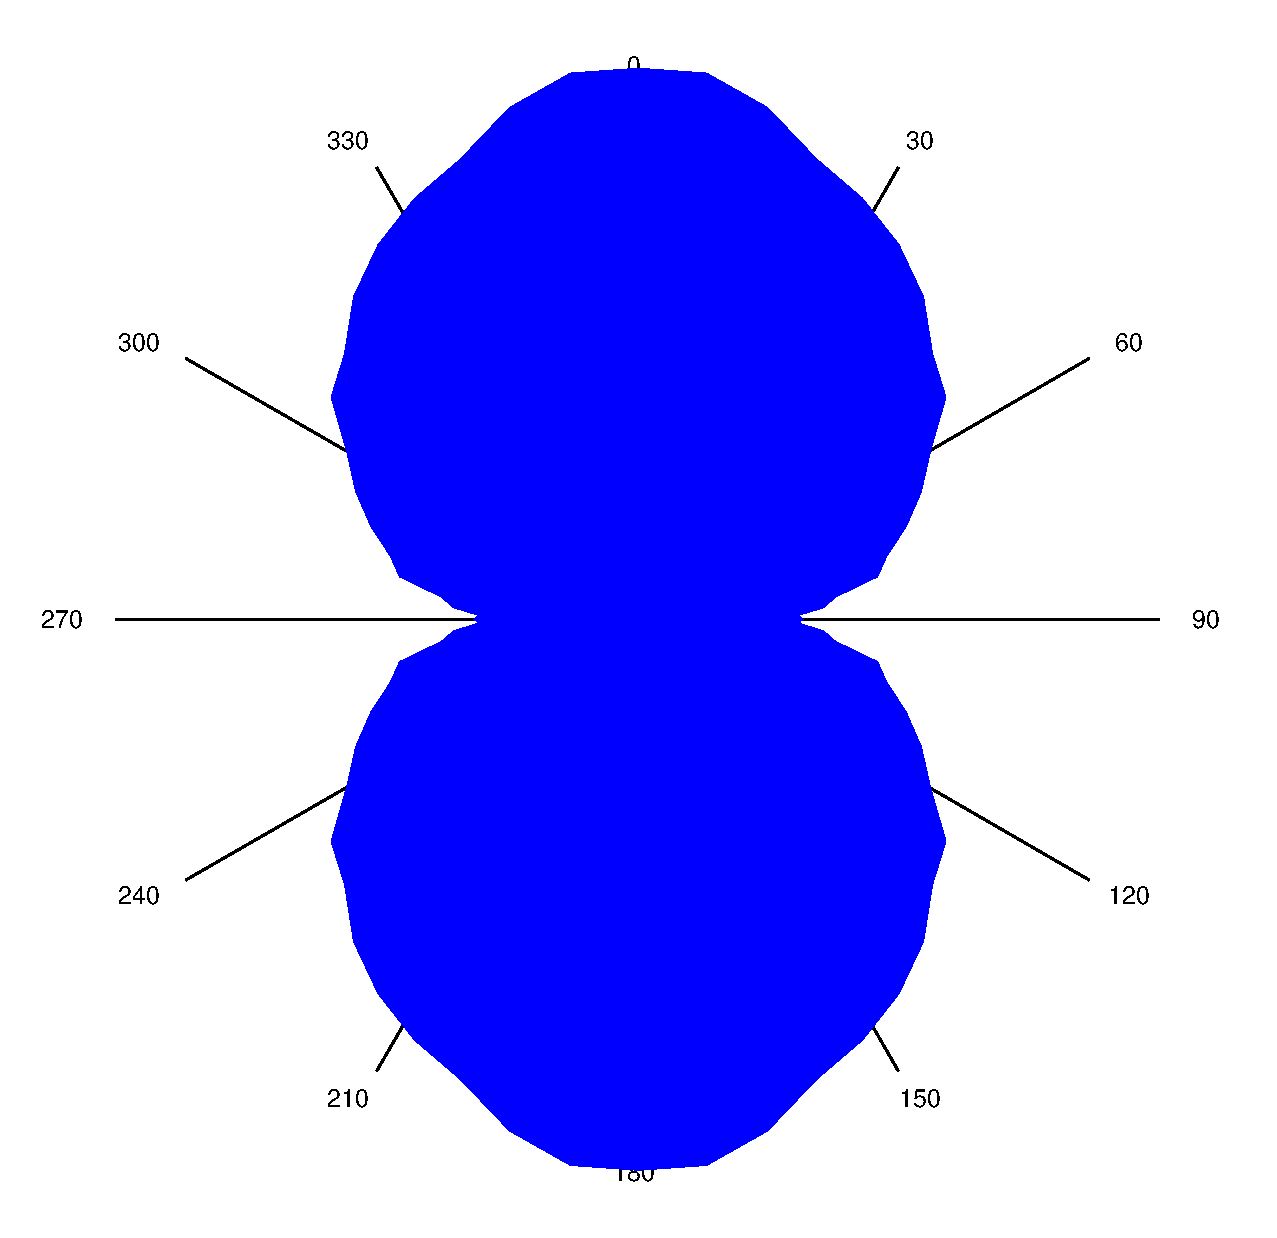
\includegraphics[scale=0.2]{FP-V23data/2.3_2306.535Hz.eps}
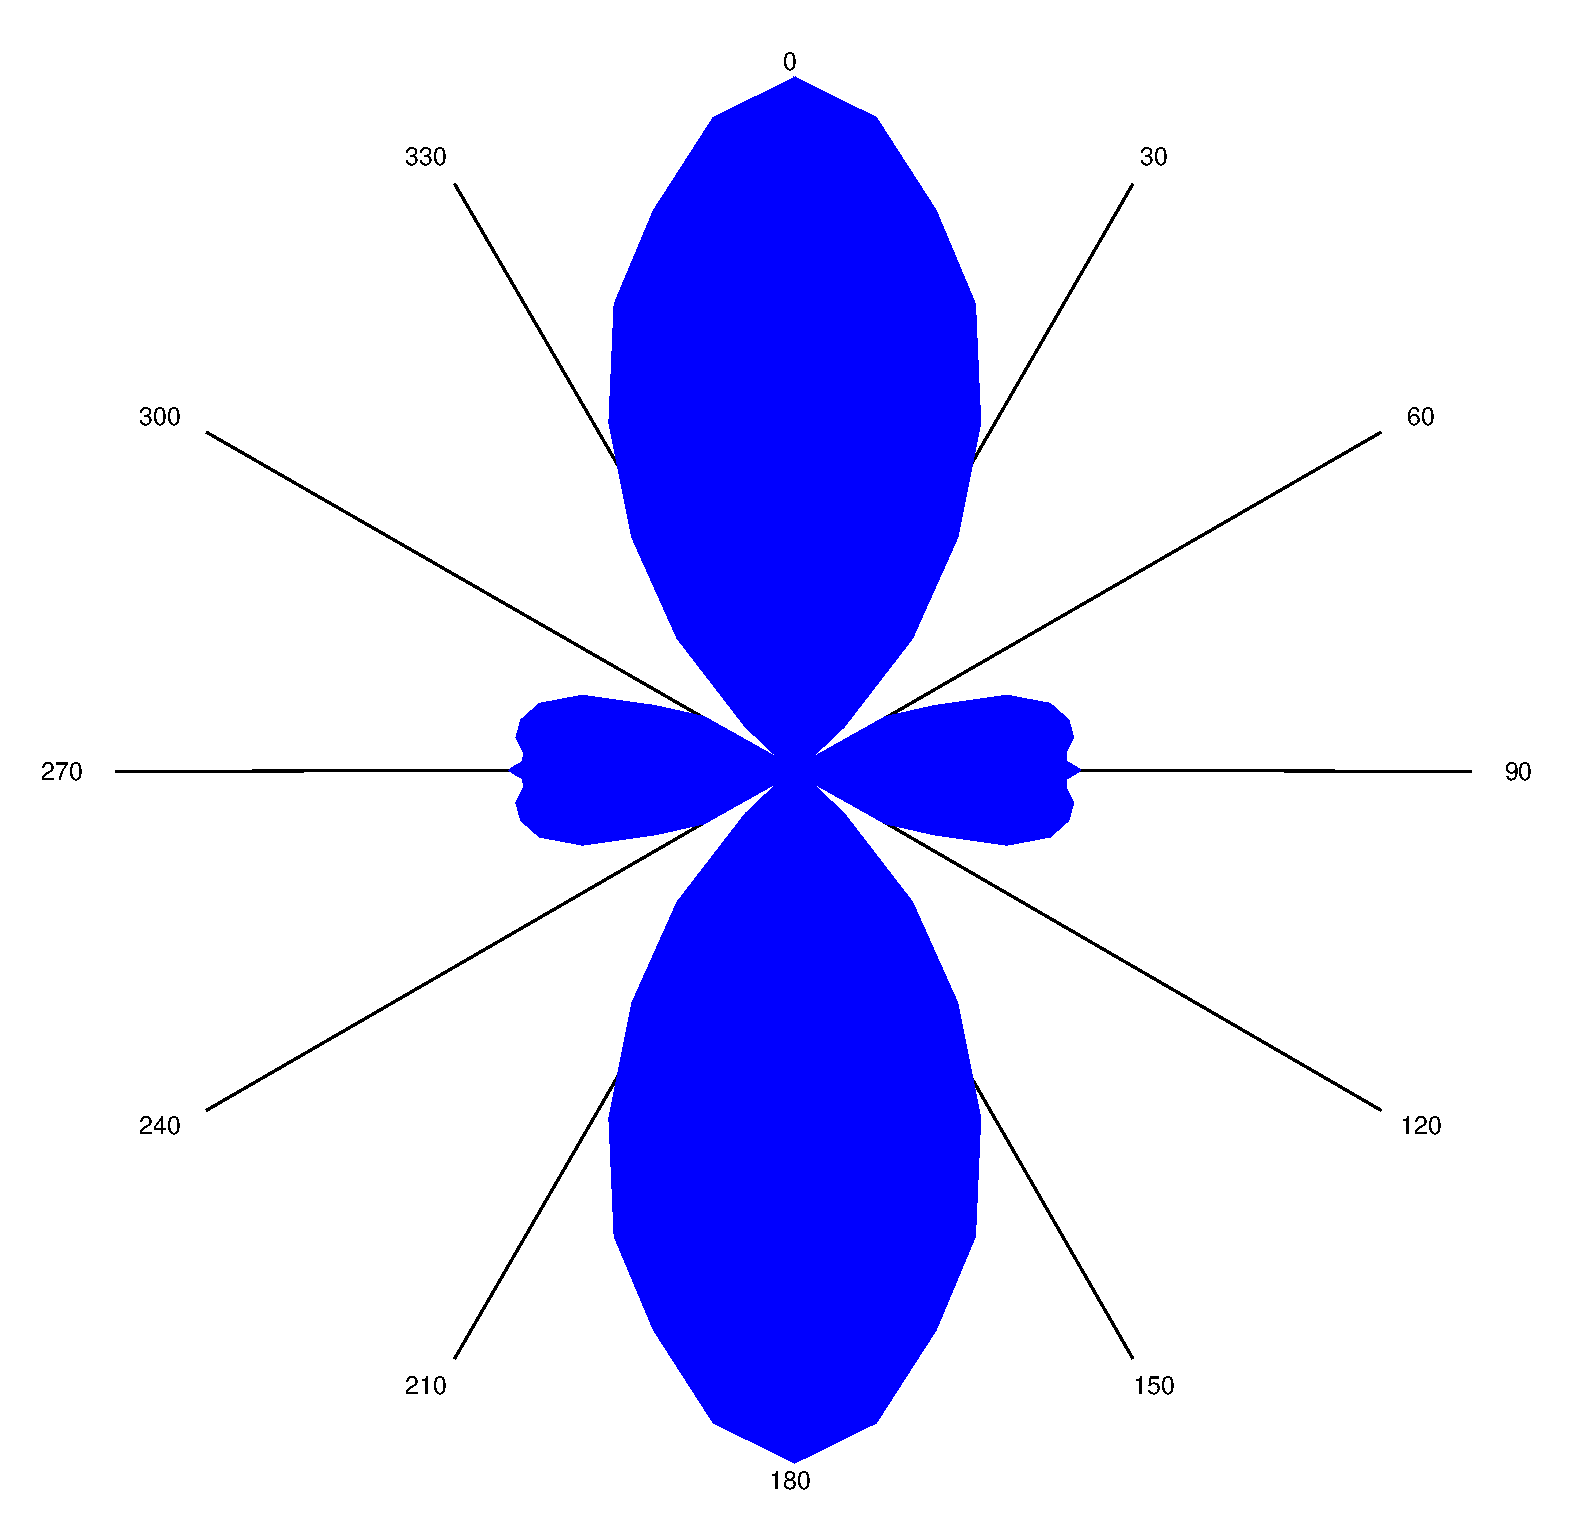
\includegraphics[scale=0.15]{FP-V23data/2.3_3704.961Hz.eps}
\end{minipage}
\begin{minipage}{0.45\textwidth}
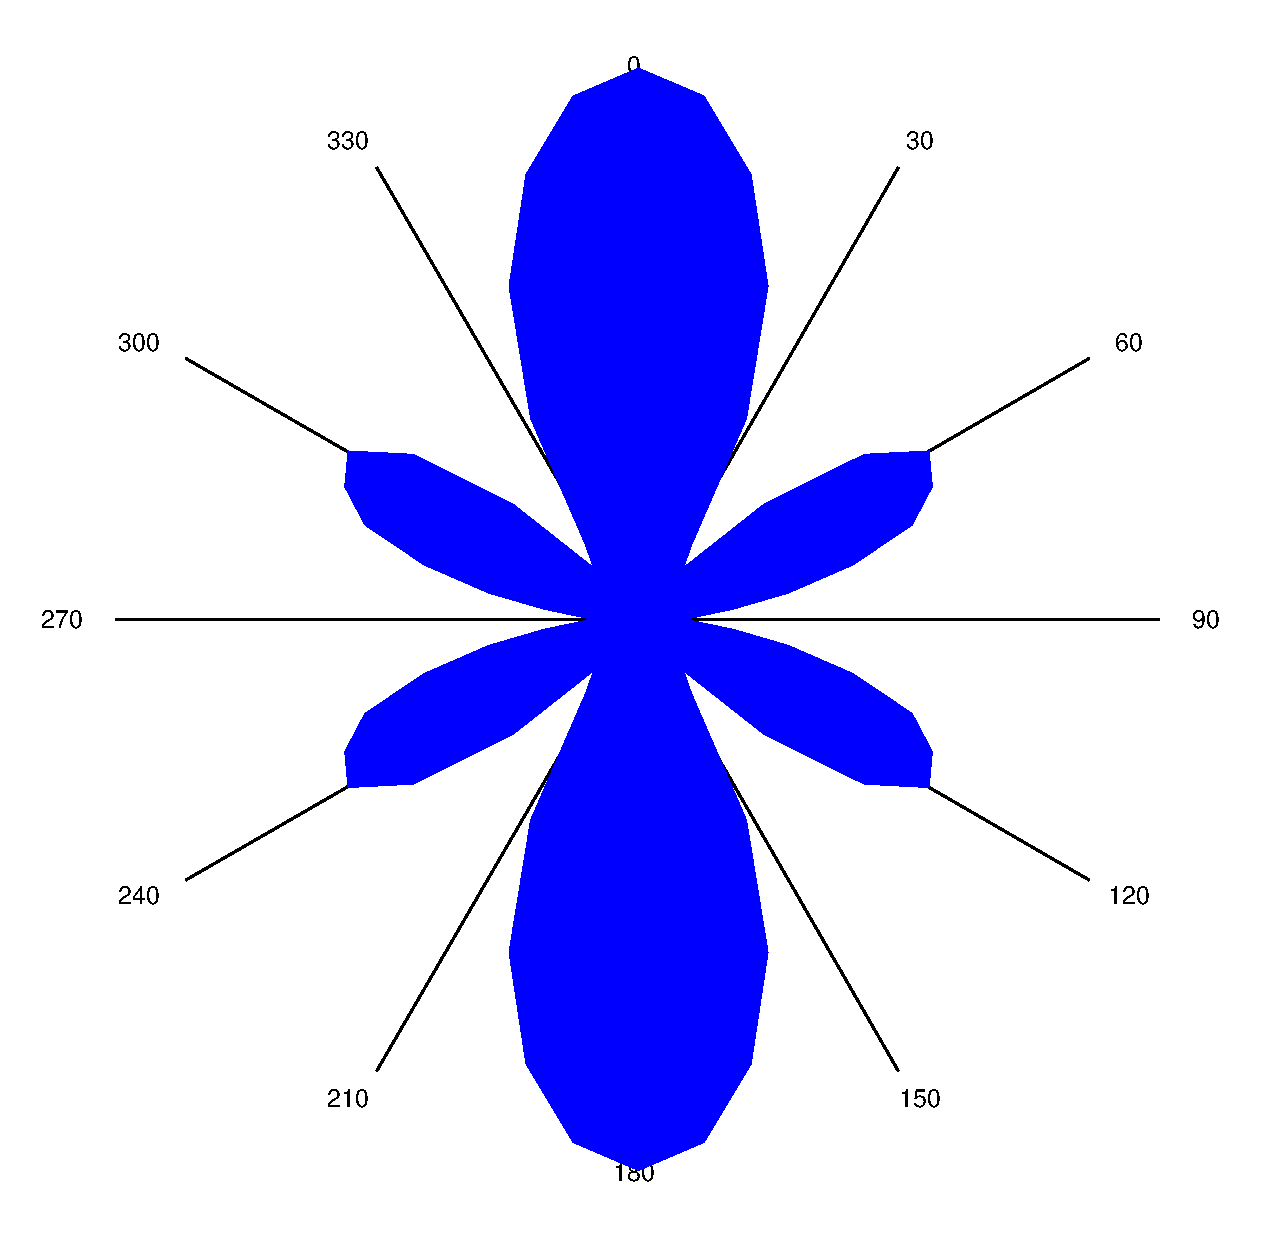
\includegraphics[scale=0.2]{FP-V23data/2.3_4985.394Hz.eps}
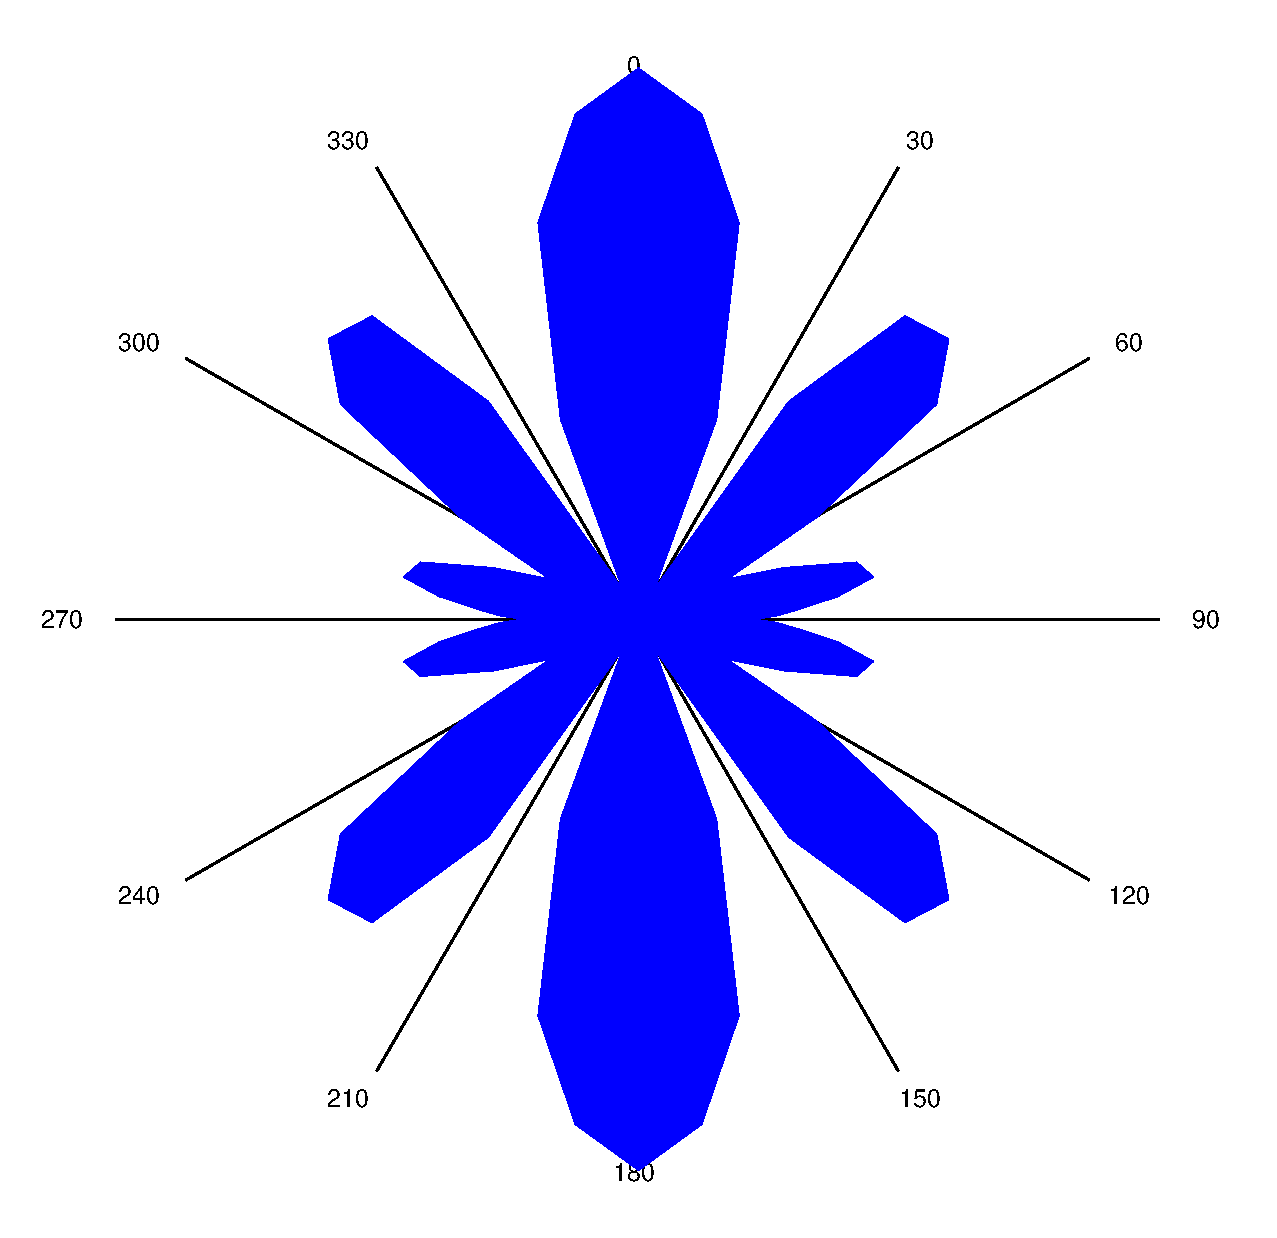
\includegraphics[scale=0.2]{FP-V23data/2.3_6230.866Hz.eps}
\end{minipage}
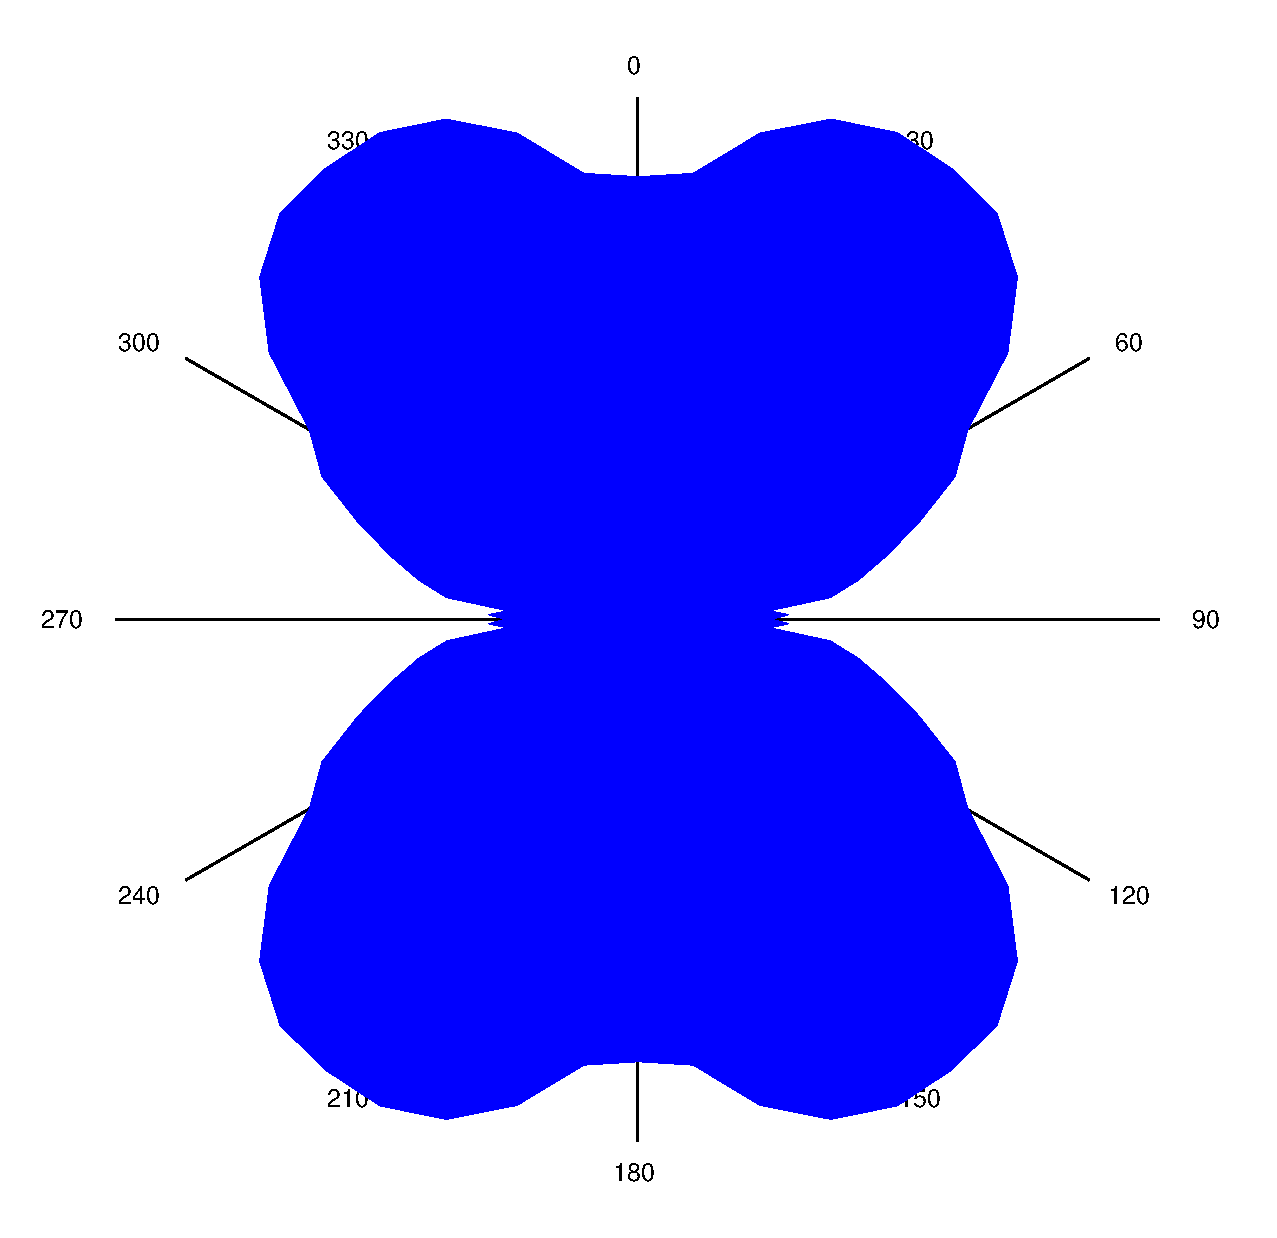
\includegraphics[scale=0.2]{FP-V23data/2.3_6571.732Hz.eps}
\caption{Polarplots der ersten fünf Peaks im sphärischen Resonator}
\label{fig:polar}
\end{figure}
\subsection{Modellierung: Ein eindimensionaler Festkörper}
\subsection{Teilchen im periodischen Potential}
In Abbildung \ref{fig:Spek4_1} ist beispielhaft das Spektrum von  $\SI{5000}{\hertz}$ bis $\SI{14000}{\hertz}$ einer $\SI{75}{\milli\meter}$-Röhre zu sehen.
Der mittlere Abstand zwischen den Peaks wird über die Formel zur Berechnung des Mittelwerts
\[
\mu_{\Delta f} = \frac{1}{N}\sum_{i=1}^{N}(\Delta f)_i
\]
und dessen Standardabweichung
\[
\sigma_{\Delta f} = \sqrt{\frac{1}{N(N-1)}\sum_{i=1}^{N}((Delta f)_i-\mu_{\Delta f})^2}
\]
bestimmt. Dasselbe wird für zwei bis acht $\SI{75}{\milli\meter}$-Röhren durchgeführt. Die berechneten Mittelwerte sind in Tabelle
\ref{tab:mu} zu sehen und sind in Abbildung \ref{fig:Df_L} gegen die Inverse der Röhrenlänge $L$ aufgetragen. Eine lineare Ausgleichsrechnung der Form $\Delta f\left(\frac{1}{L}\right)= a\cdot\frac{1}{L}+b$ liefert die Parameter
\begin{align*}
a&=\SI{}{\meter\per\second}\\
b&=\SI{}{\second^{-1}}\text{.}
\end{align*}
Ein Koeffizientenvergleich mit Gleichung \eqref{eq:f} liefert für die Schallgeschwindigkeit $c$ die Beziehung
\[
c=2 a=\SI{}{\meter\per\second}\text{.}
\]
\newline
In Abbildung \ref{fig:12_50} ist das Spektrum von zwölf $\SI{50}{\milli\meter}$-Röhren zu sehen und in Abbildung \ref{fig:w_k} werden als Dispersionsrelation die Winkelfrequenzen der Peaks $\omega_n=2\pi f_n$ gegen die zugehörigen Wellenzahlen $k_n$ aufgetragen. Eine lineare Ausgleichsrechnung der Form $\omega(k)=c k + d$ liefert die Parameter
\begin{align*}
c&=\SI{}{\meter\per\second}\\
d&=\SI{}{\second^{-1}}\text{.}
\end{align*}
Ein Vergleich mit Gleichung \eqref{eq:w_k} zeigt das $c$ der Schallgeschwindigkeit entspricht.\\
In Abbildung \ref{fig:8_50_16} ist das Spektrum von acht über $\SI{16}{\milli\meter}$-Irisse gekoppelten $\SI{50}{\milli\meter}$-Röhren zu sehen. Dieselbe Messung wird für $10$- und $\SI{13}{\milli\meter}$-Kopplungen durchgeführt und die jeweiligen Dispersionsrelationen in den Abbildungen \ref{fig:w_k_1} bis \ref{fig:w_k_3} aufgetragen.\\
%Tabelle der Band-/Bandlückenbreiten?
In den Abbildungen \ref{fig:10_50_16} und \ref{fig_12_50_16} sind die Spektren für zehn und zwölf über $\SI{16}{\milli\meter}$-Irisse gekoppelte $\SI{50}{\milli\meter}$-Röhren zu sehen. Im Vergleich zu \ref{fig:8_50_16} zeigt sich, dass während die Lage der Peaks  mit zunehmender Röhrenlänge nahezu unverändert ist, die Amplitude aller Peaks mit Ausnahme des ersten abfallen, während dieser stark anwächst. Außerdem wächst für größere $L$ die Anzahl der Peaks pro Band.\\
In Abbildung \ref{fig:8_75_16} ist das Spektrum von acht über $\SI{16}{\milli\meter}$-Irisse gekoppelten $\SI{75}{\milli\meter}$-Röhren zu sehen. Der Vergleich mit Abbildung \ref{fig:8_50_16} zeigt, das bei längeren Teilstücken die Amplitude der Peaks sowie die Anzahl der beobachtbaren Bänder zunimmt.\\
%density of states?
\begin{figure}
\centering
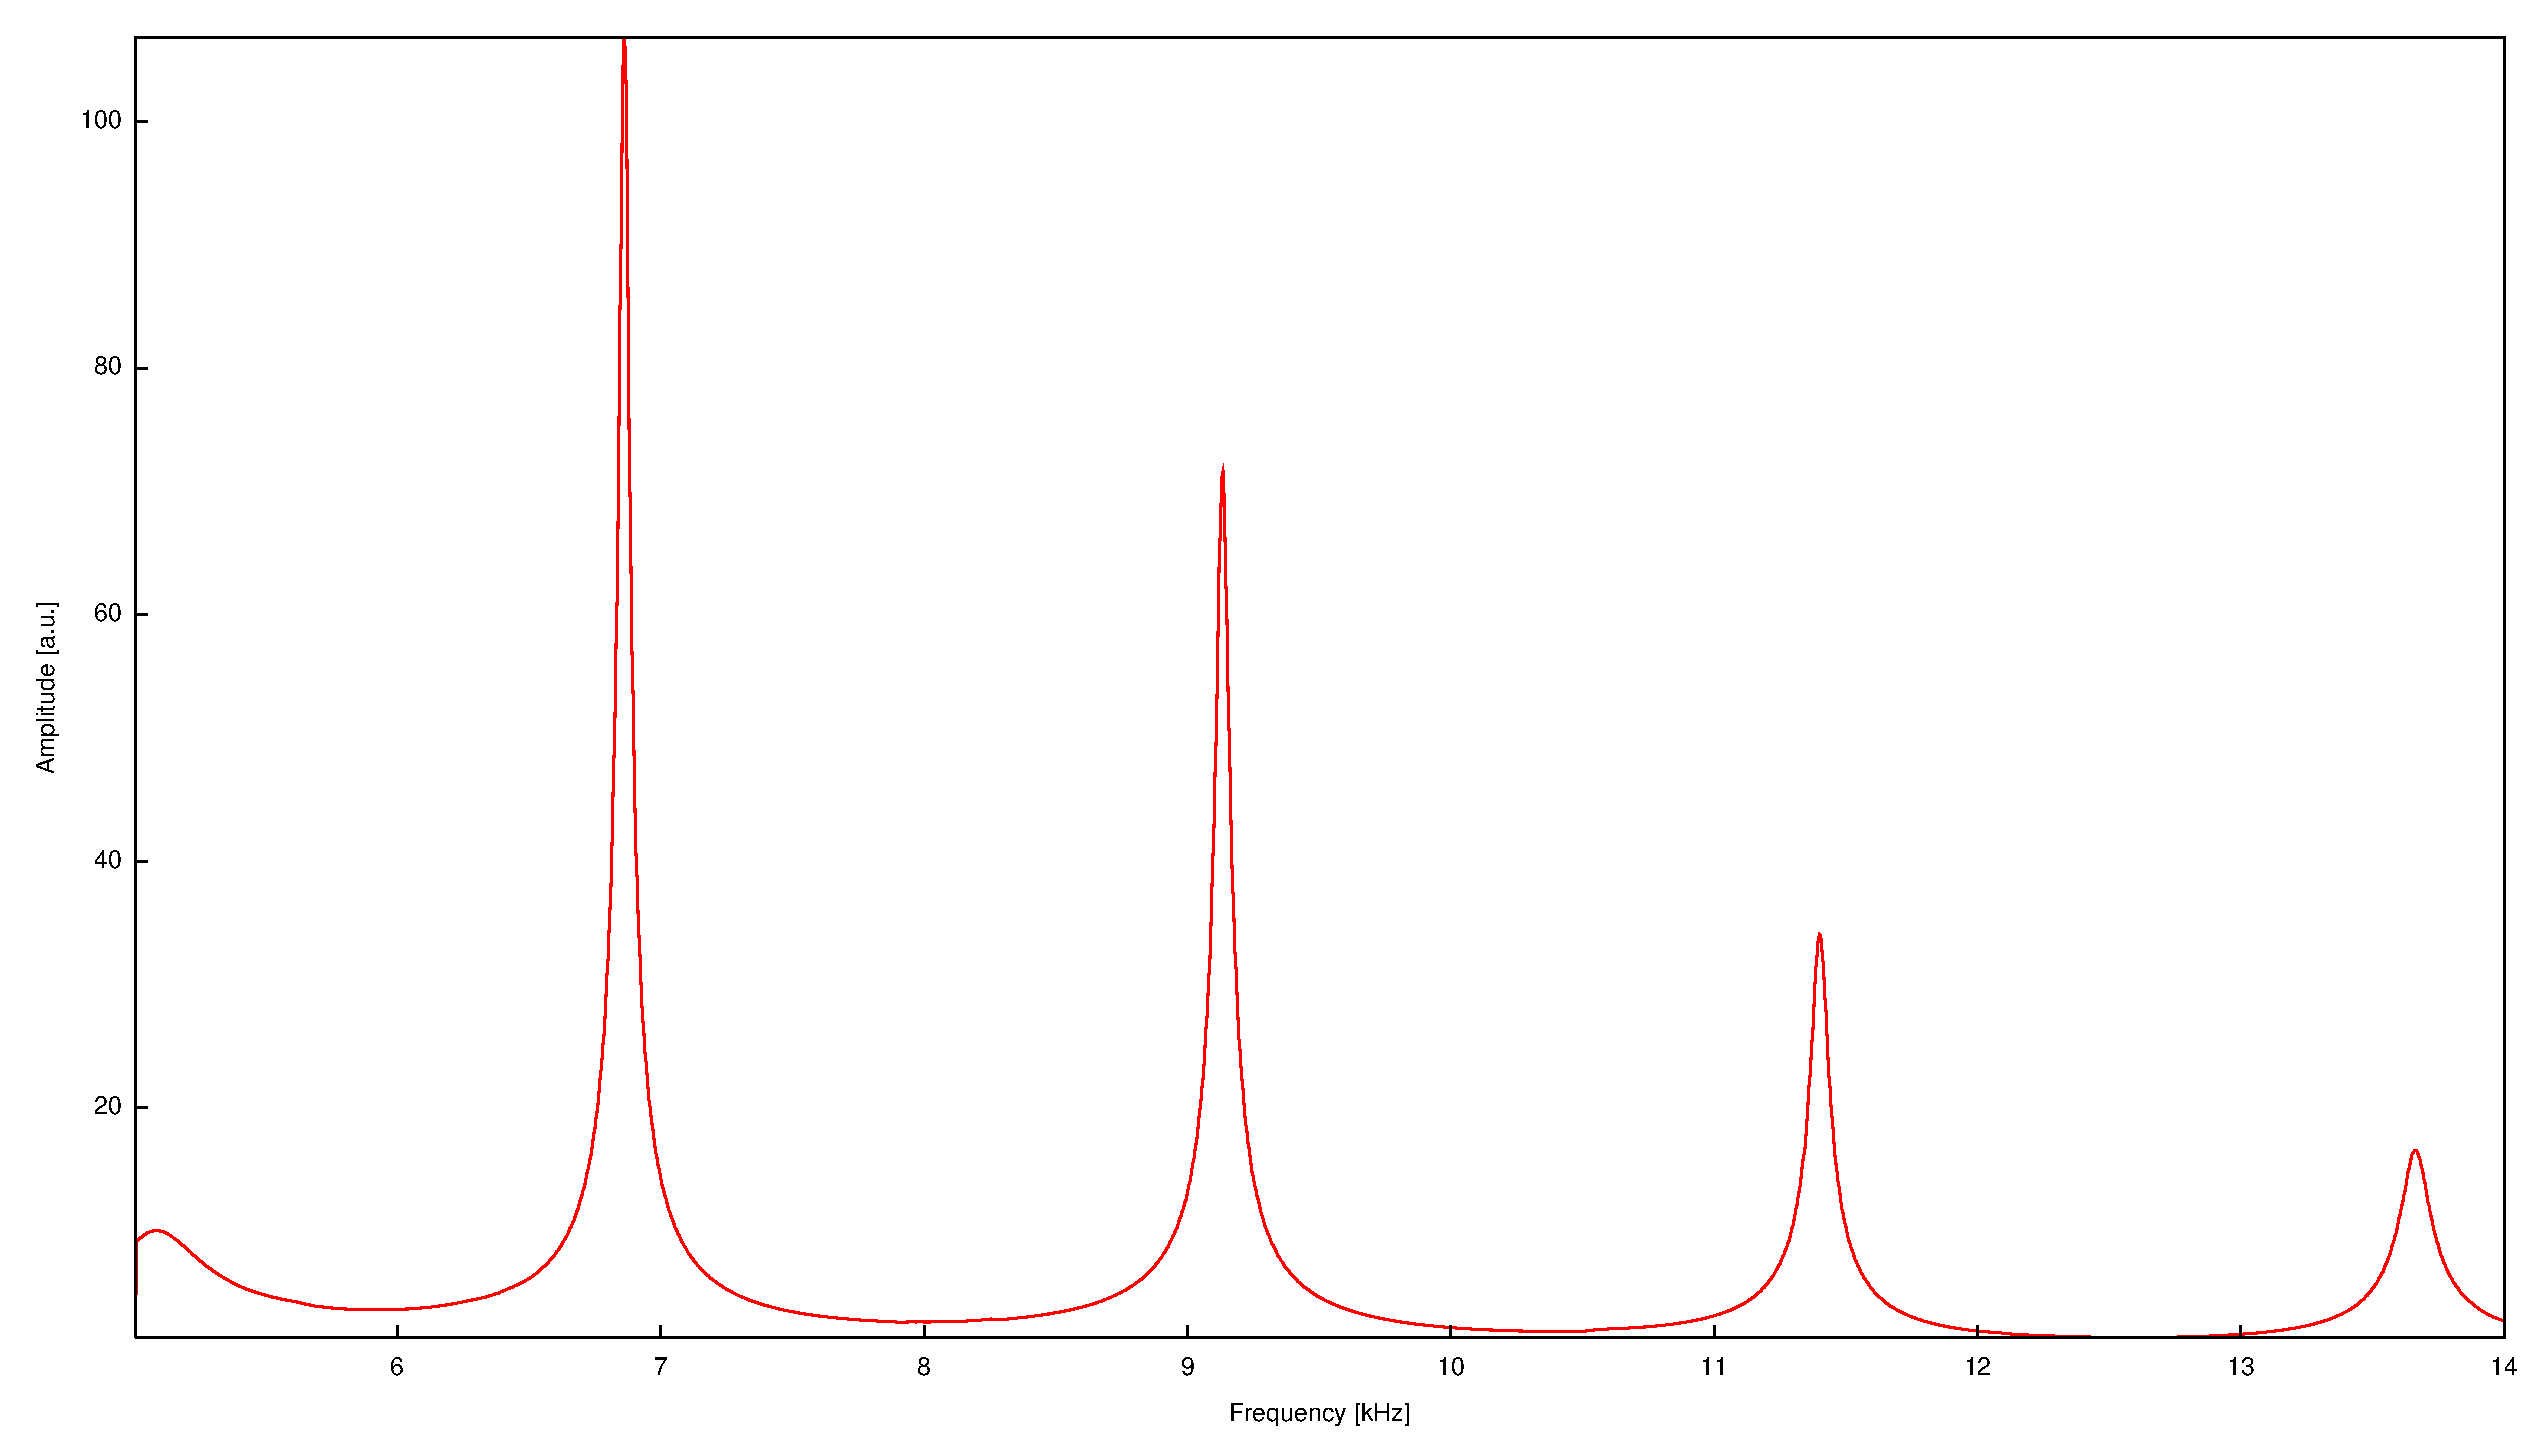
\includegraphics[width=\linewidth-60pt,height=\textheight-60pt,keepaspectratio]{FP-V23data/4.1_75mm.eps}
\caption{Spektrum von einer $\SI{75}{\milli\meter}$-Röhre.}
\label{fig:Spek4_1}
\end{figure}
\begin{table}
\centering
\caption{Mittlerer Abstand der Peaks}
\label{tab:mu}
	\sisetup{table-format=1.2}
	\begin{tabular}{S[table-format=3.0]r@{${}\pm{}$}l}
		\toprule
		{$L/(\si{\milli\meter})$} & \multicolumn{2}{c}{$\Delta f/(\si{\second^{-1}})$} \\
		\midrule
		 75 & 2268.3 & 3.3 \\
		 150 & 11393 & 2.5 \\
		 225 & 763.3 & 1.4 \\
		 300 & 573.5 & 1.3 \\
		 375 & 458.6 & 1.2 \\
		 450 & 382.7 & 0.9 \\
		 525 & 327.1 & 0.7 \\
		 600 & 286.6 & 0.6 \\
		\bottomrule
	\end{tabular}

\end{table}
\begin{figure}
\centering
\includegraphics[width=\linewidth-60pt,height=\textheight-60pt,keepaspectratio]{build/4.1.pdf}
\caption{$\Delta f$ aufgetragen gegen $\frac{1}{L}$ zur Bestimmung der Schallgeschwindigkeit $c$.}
\label{fig:Df_L}
\end{figure}
\begin{figure}
\centering
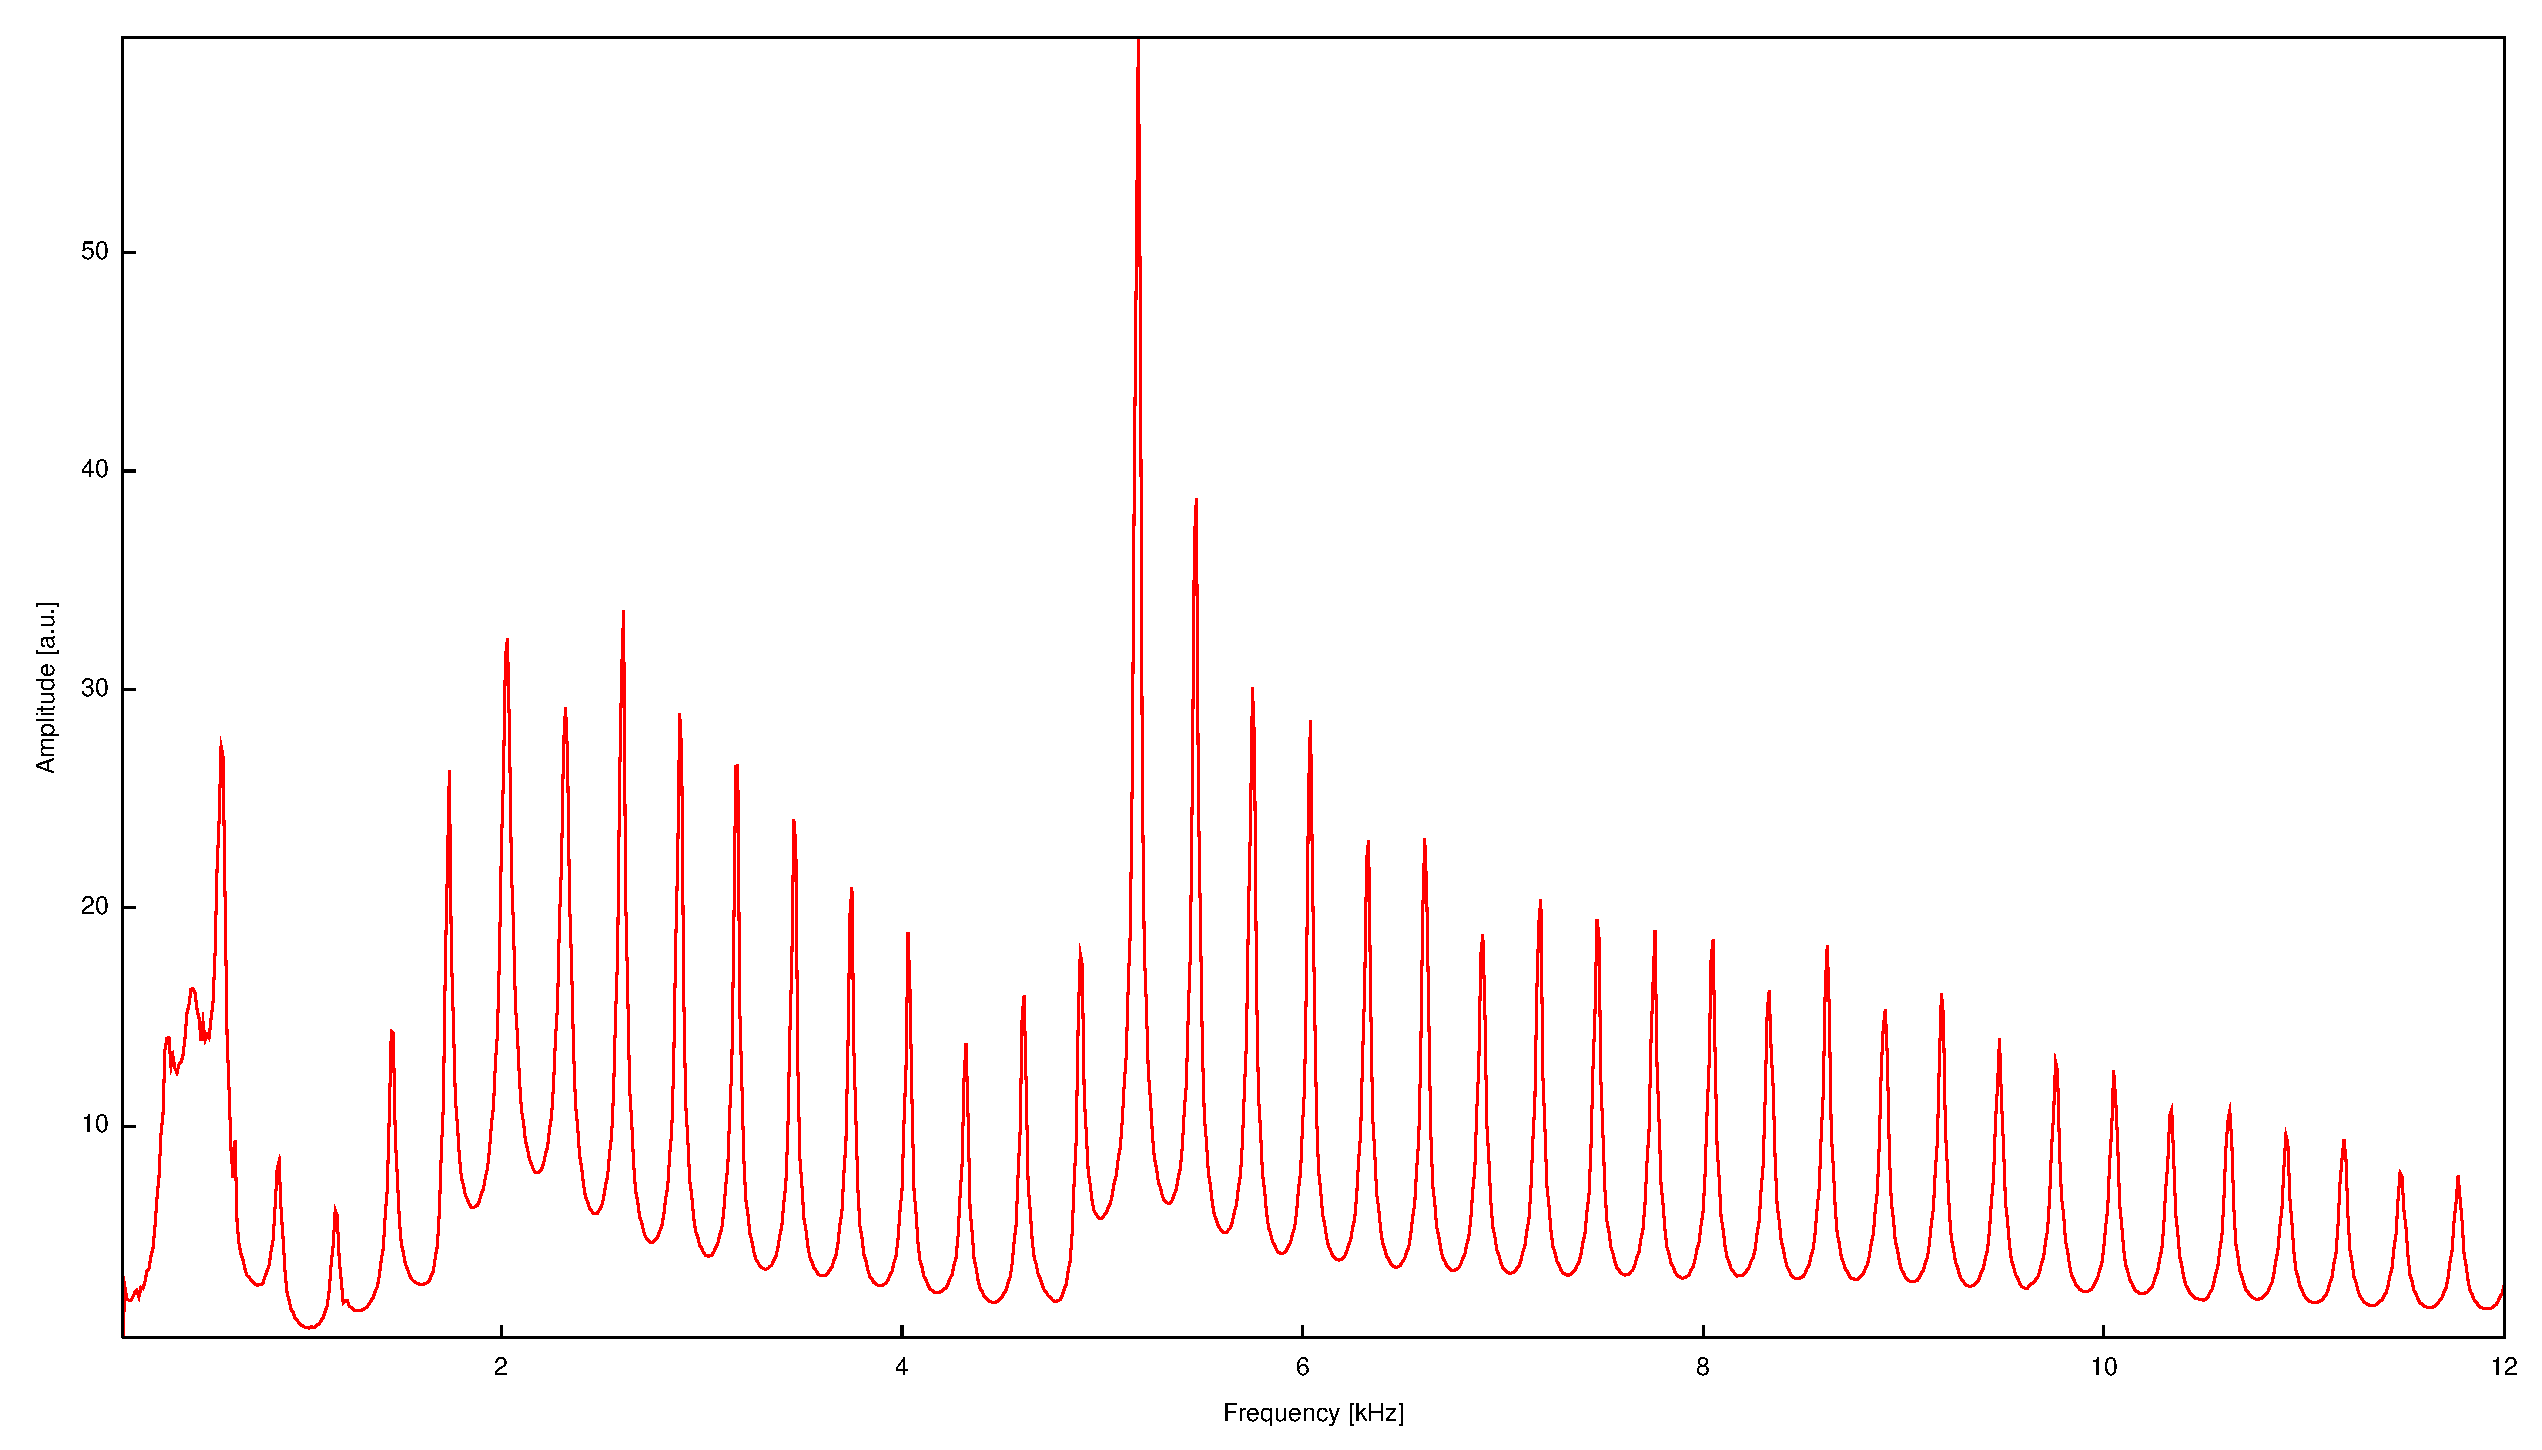
\includegraphics[width=\linewidth-60pt,height=\textheight-60pt,keepaspectratio]{FP-V23data/4.2_600mm.eps}
\caption{Spektrum von zwölf $\SI{50}{\milli\meter}$-Röhren.}
\label{fig:12_50}
\end{figure}
\begin{figure}
\centering
\includegraphics[width=\linewidth-60pt,height=\textheight-60pt,keepaspectratio]{build/4.2.pdf}
\caption{Dispersionsrelation $\omega(k)$ von zwölf $\SI{50}{\milli\meter}$-Röhren}
\label{fig:w_k}
\end{figure}
%\begin{figure}
%\centering
%\includegraphics[width=\linewidth-60pt,height=\textheight-60pt,keepaspectratio]{build/4.3_10mm.pdf}
%\caption{•}
%\label{fig:w_k_1}
%\end{figure}
%\begin{figure}
%\centering
%\includegraphics[width=\linewidth-60pt,height=\textheight-60pt,keepaspectratio]{build/4.3_13mm.pdf}
%\caption{•}
%\label{fig:w_k_2}
%\end{figure}
%\begin{figure}
%\centering
%\includegraphics[width=\linewidth-60pt,height=\textheight-60pt,keepaspectratio]{build/4.3_16mm.pdf}
%\caption{•}
%\label{fig:w_k_3}
%\end{figure}
\begin{figure}
\centering
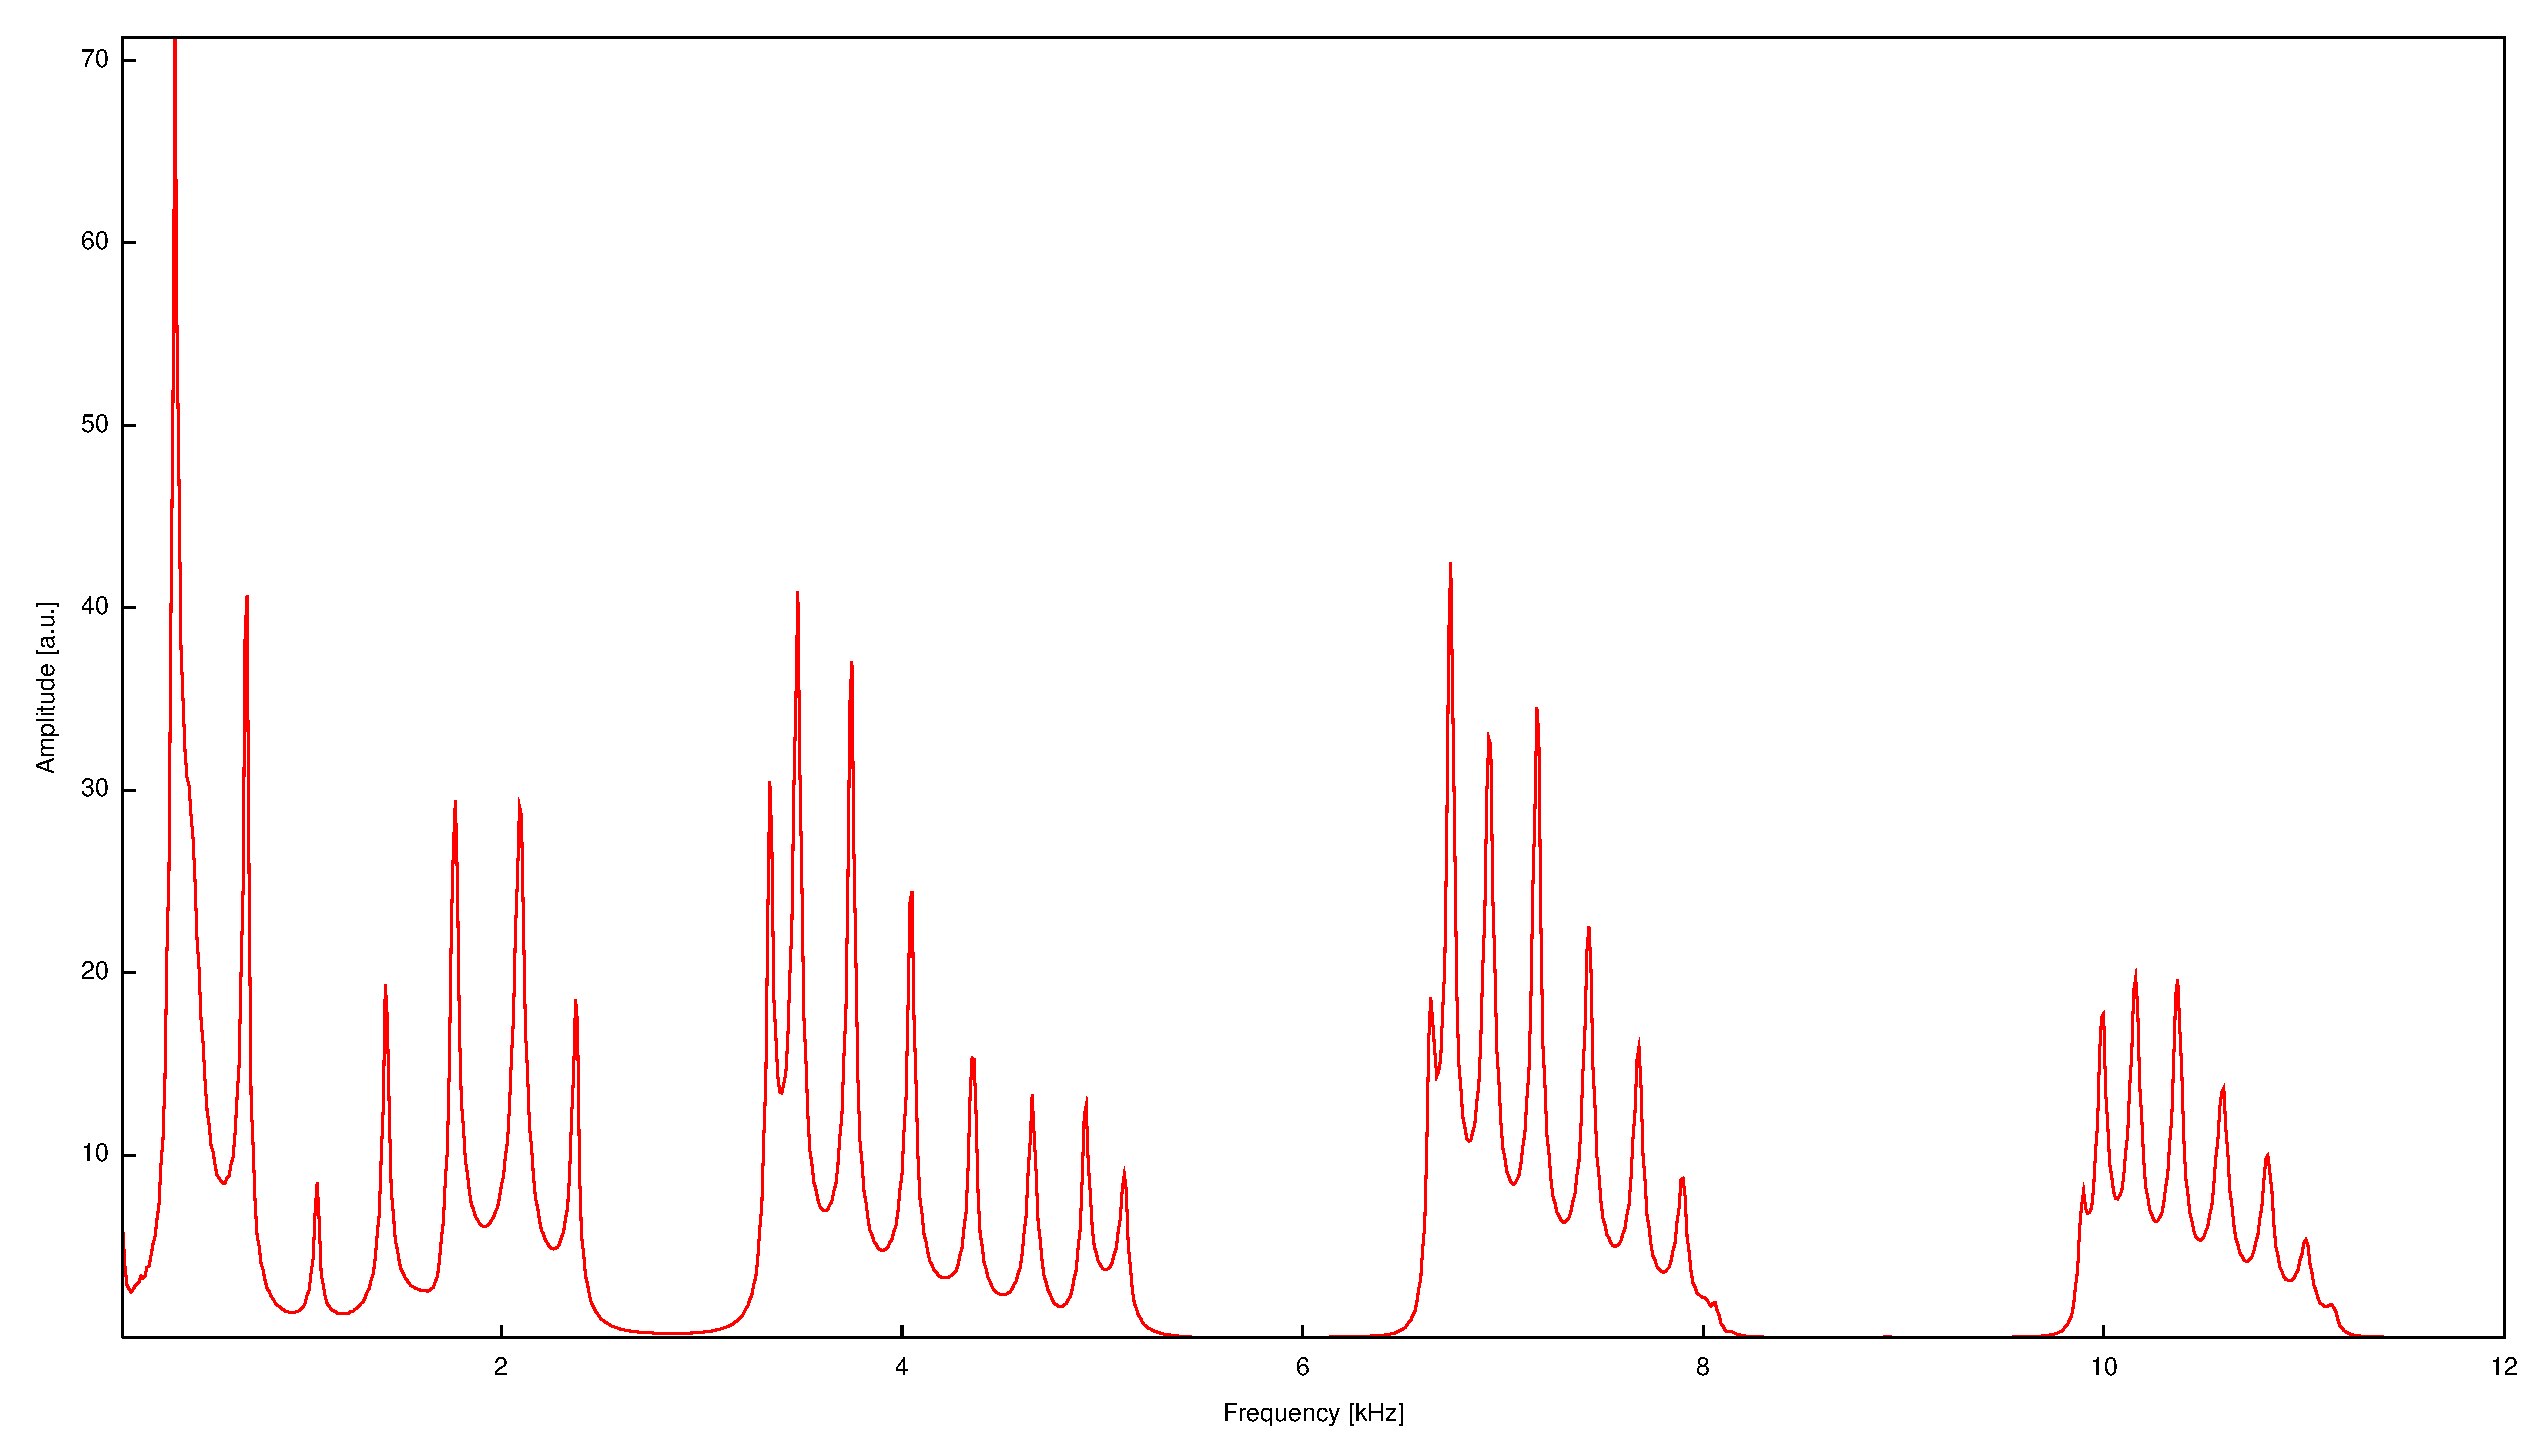
\includegraphics[width=\linewidth-60pt,height=\textheight-60pt,keepaspectratio]{FP-V23data/4.3_400mm_16mm.eps}
\caption{Spektrum von acht über $\SI{16}{\milli\meter}$-Irisse gekoppelten $\SI{50}{\milli\meter}$-Röhren}
\label{fig:8_50_16}
\end{figure}
\begin{figure}
\centering
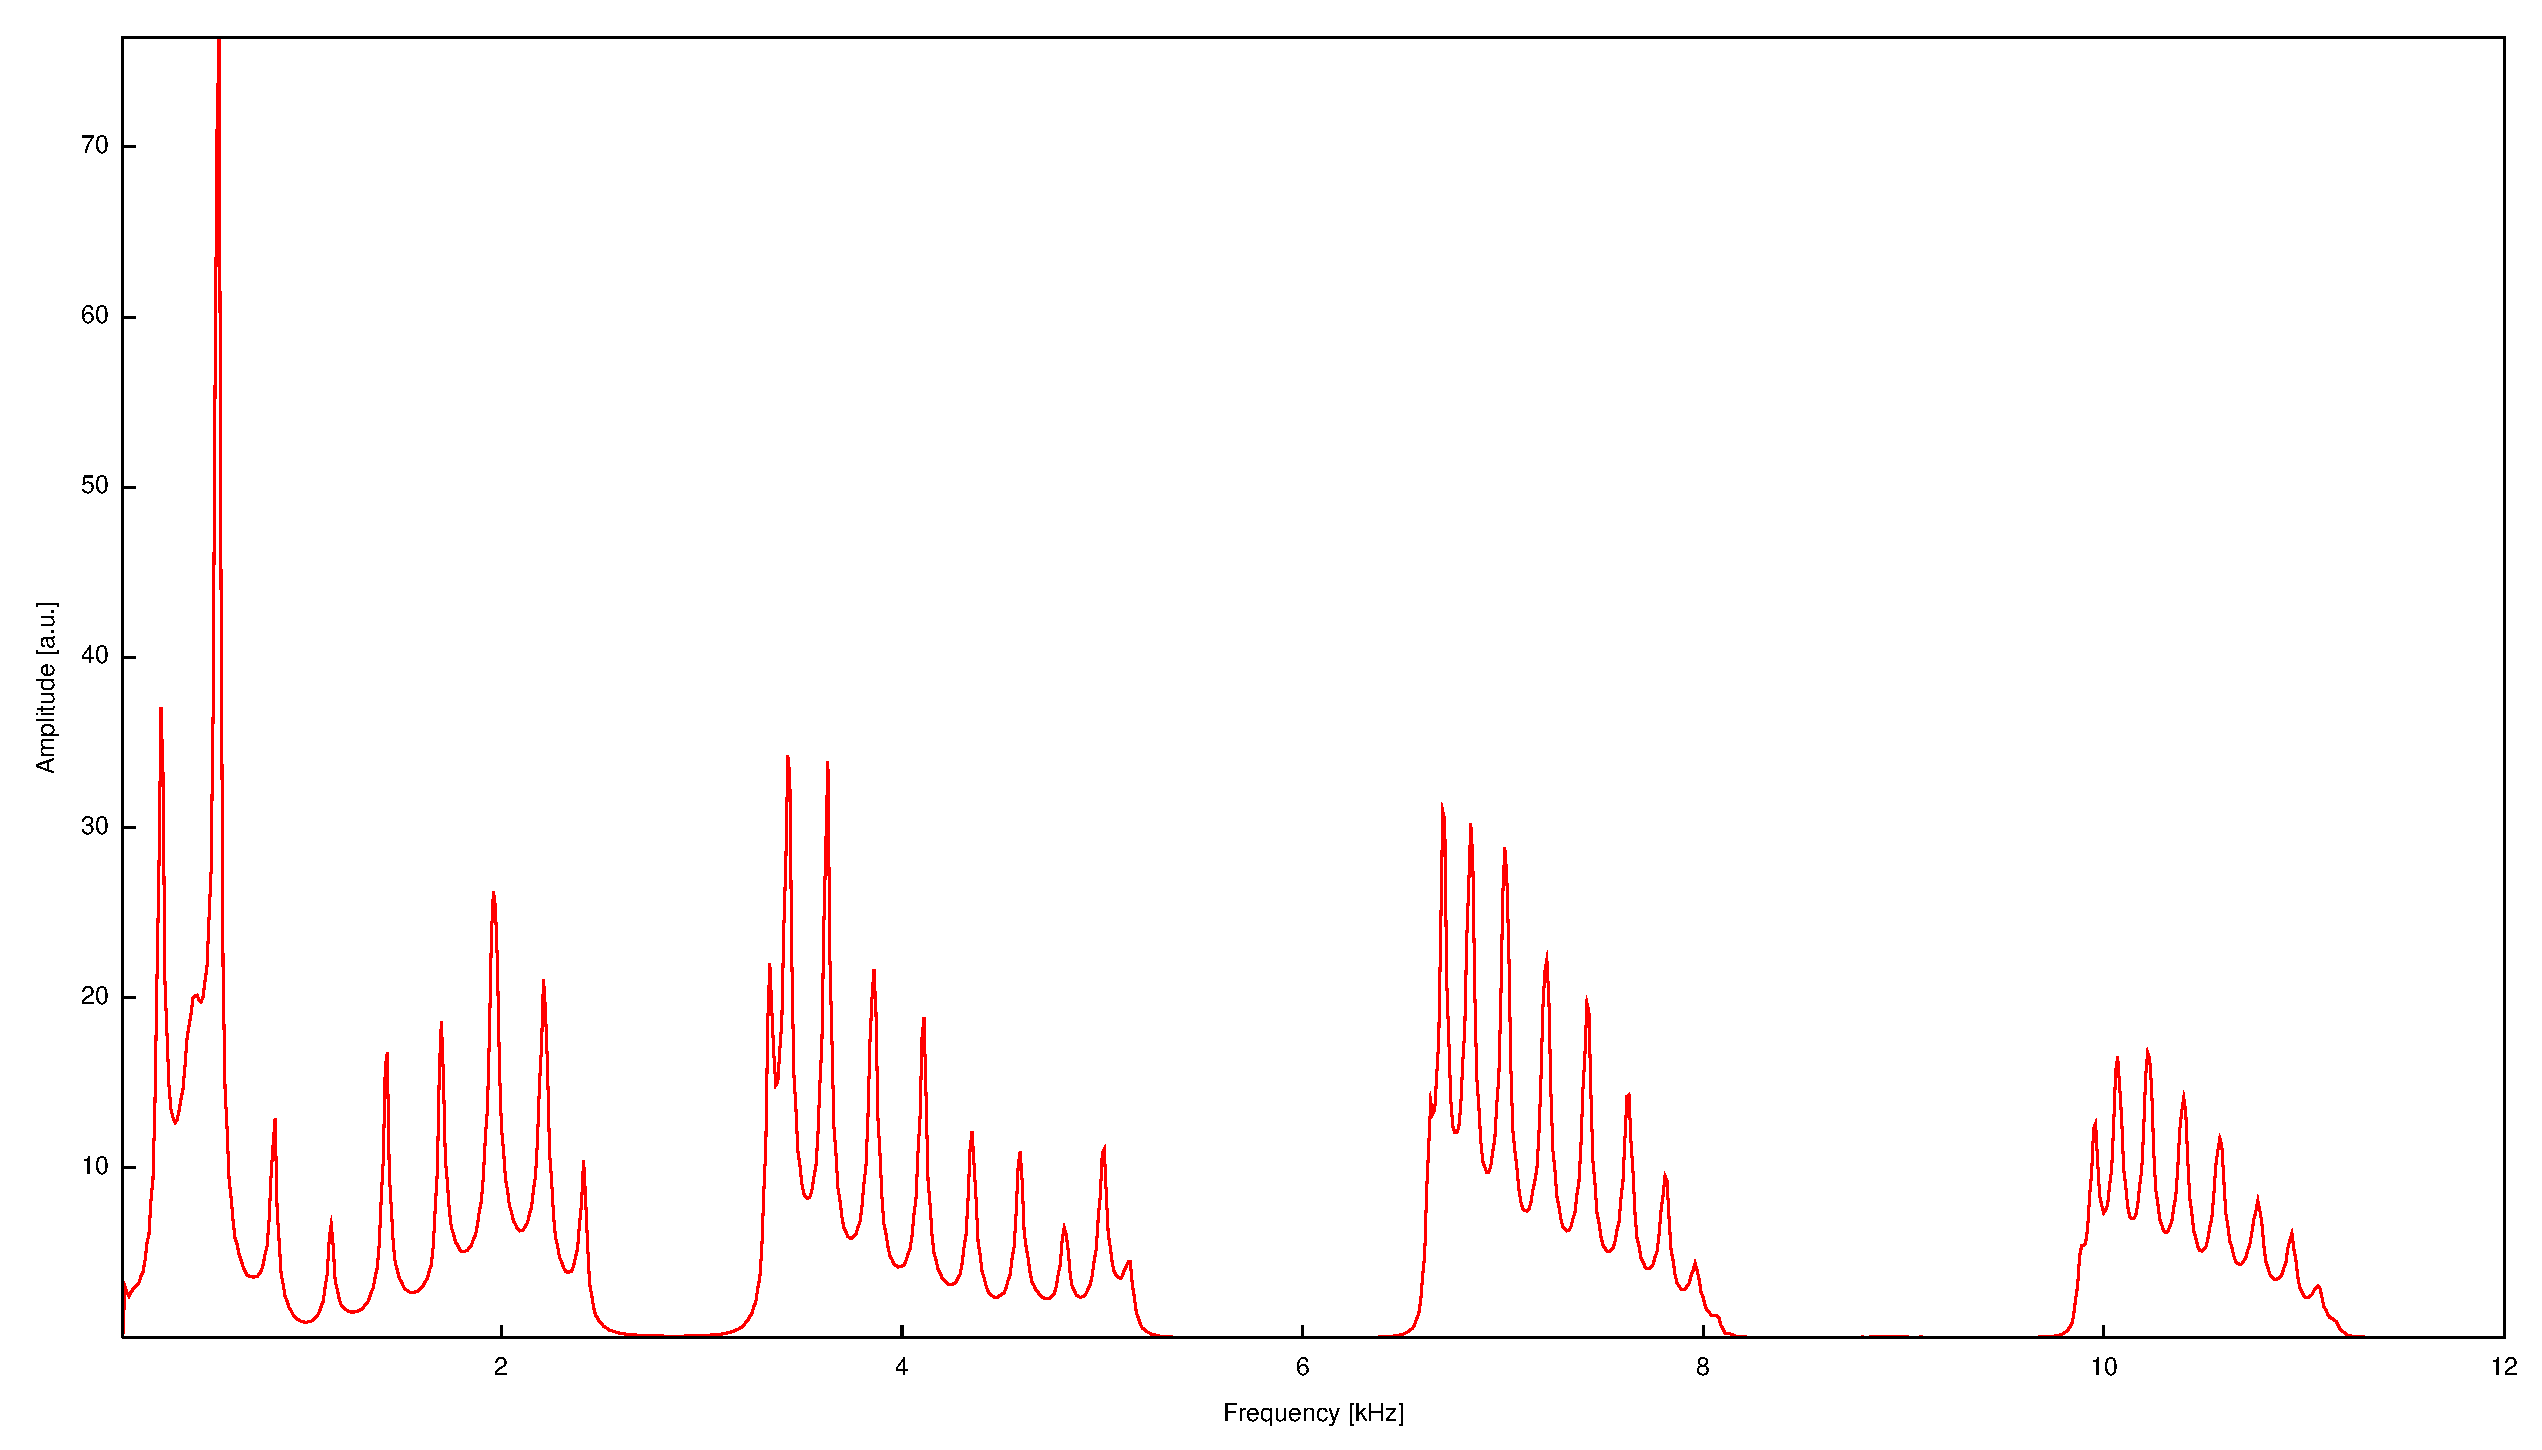
\includegraphics[width=\linewidth-60pt,height=\textheight-60pt,keepaspectratio]{FP-V23data/4.4_500mm_16mm.eps}
\caption{Spektrum von zehn über $\SI{16}{\milli\meter}$-Irisse gekoppelten $\SI{50}{\milli\meter}$-Röhren}
\label{fig:10_50_16}
\end{figure}
\begin{figure}
\centering
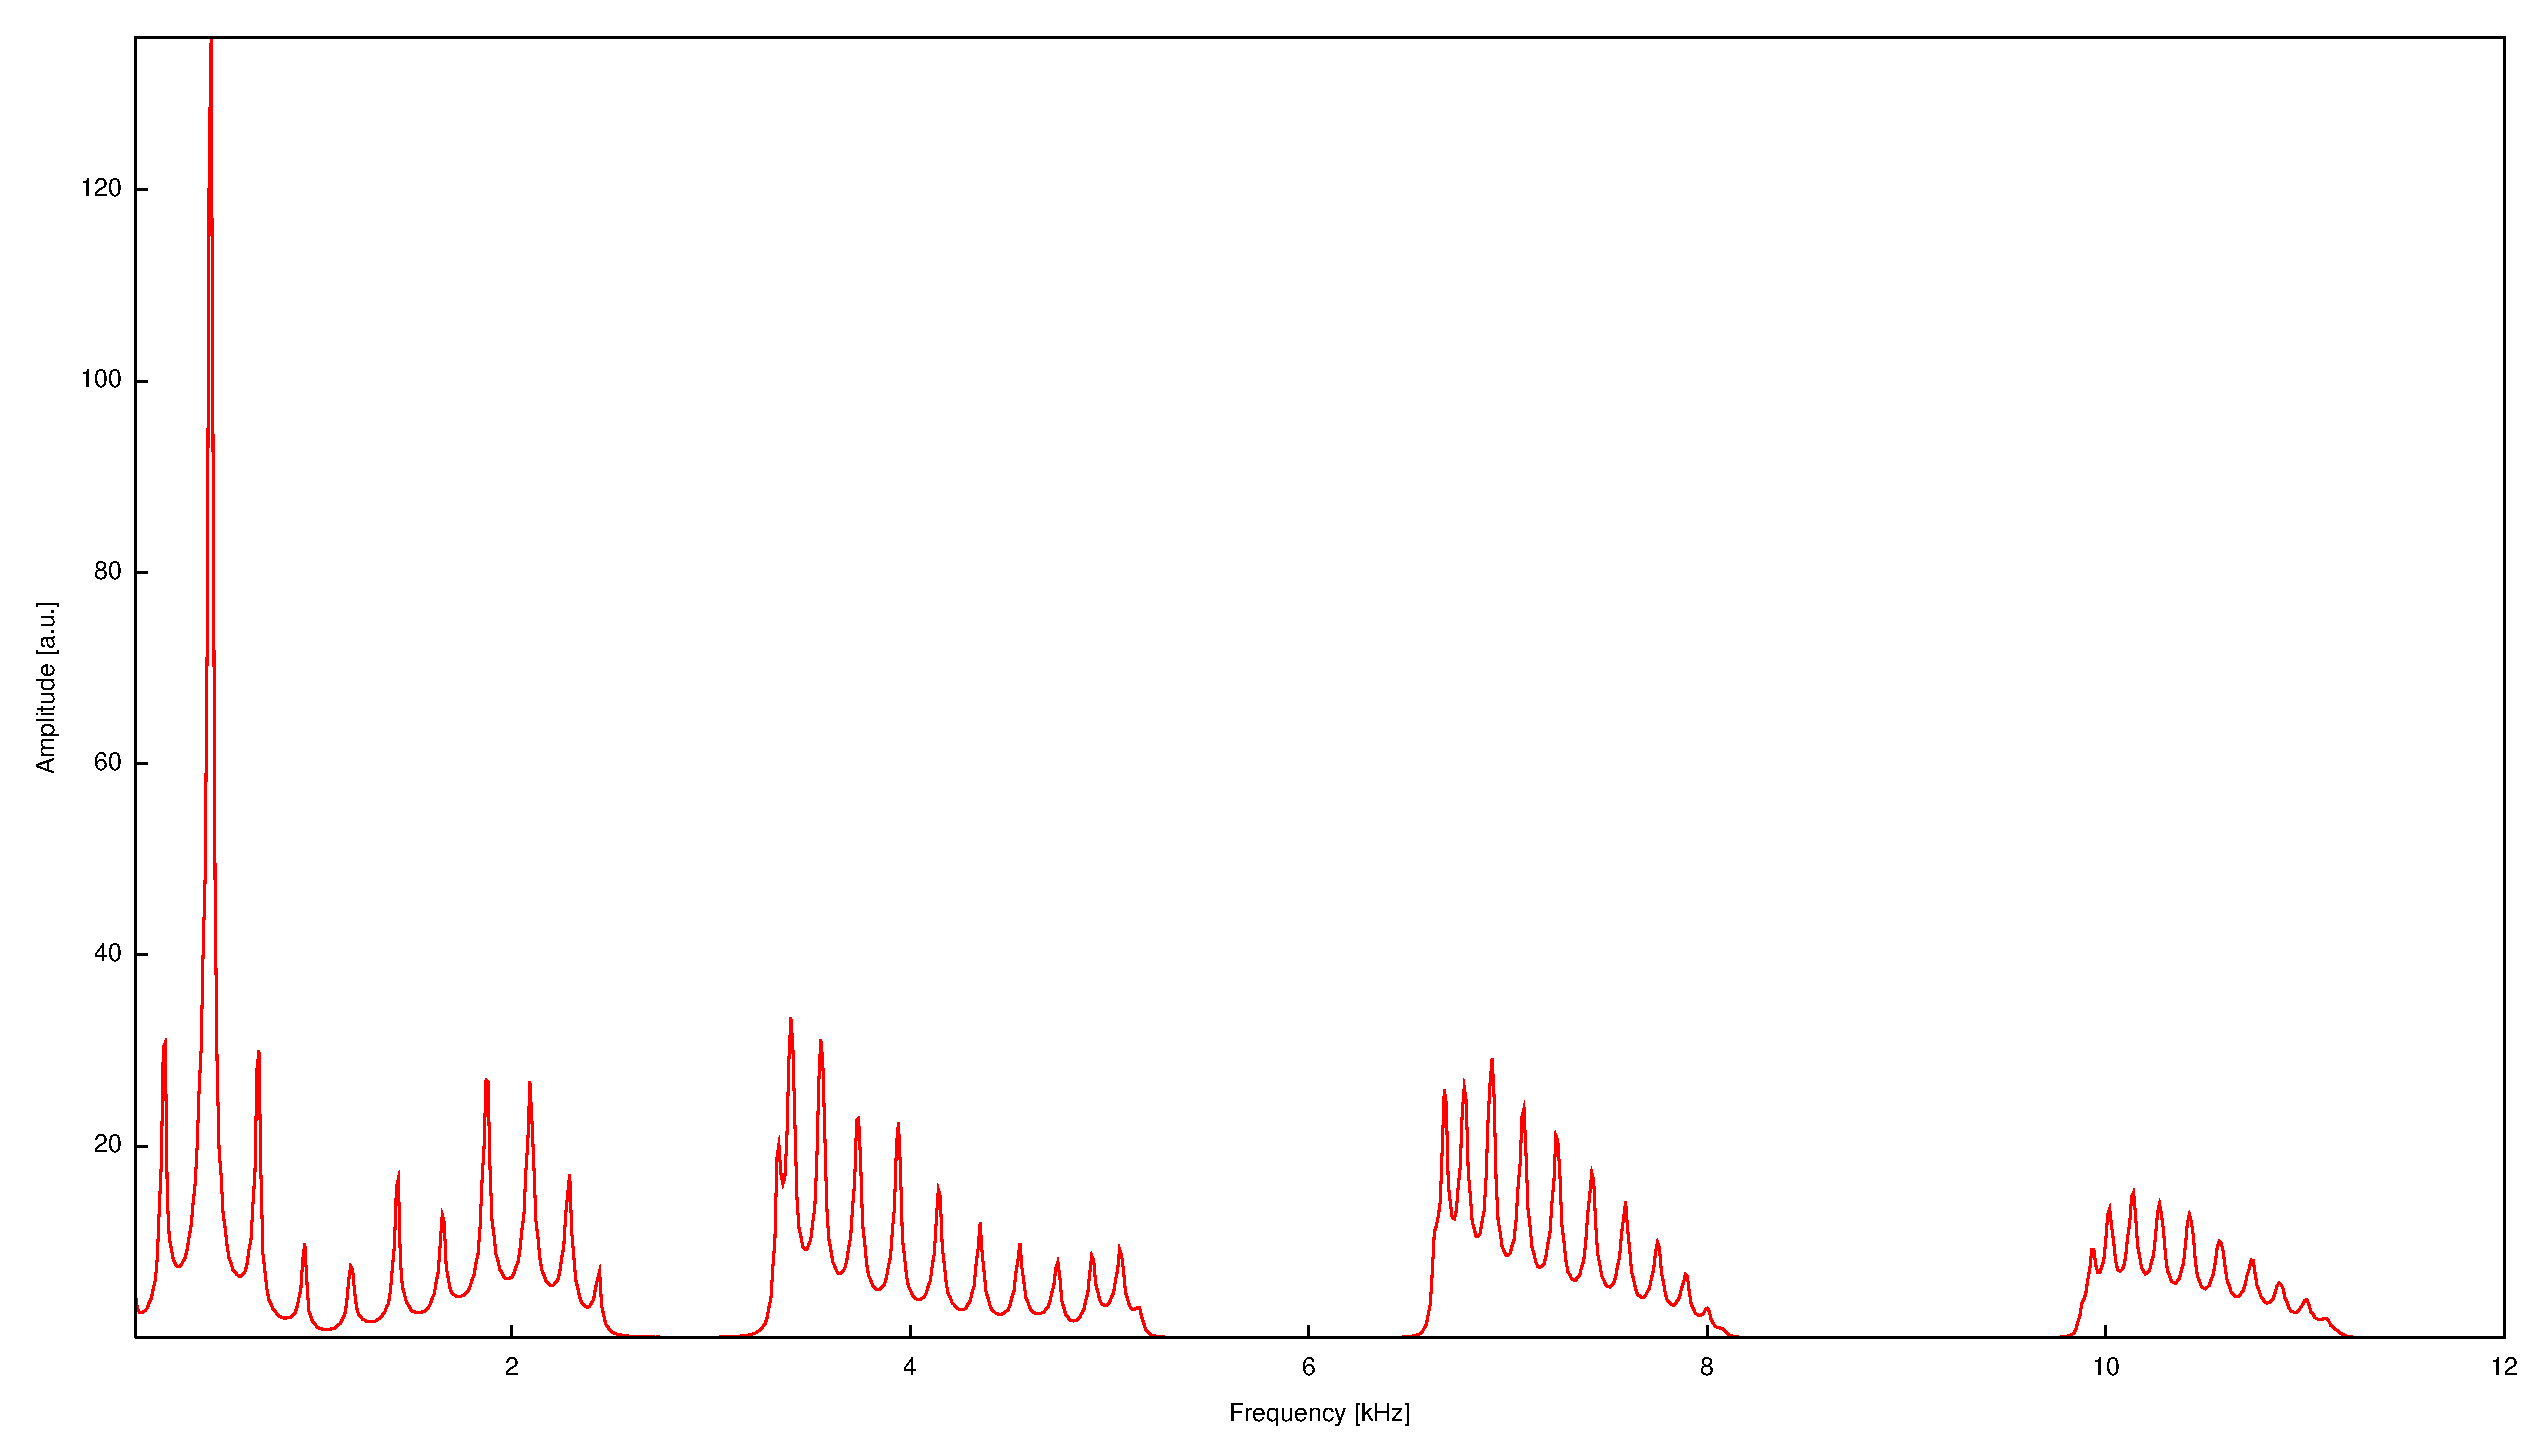
\includegraphics[width=\linewidth-60pt,height=\textheight-60pt,keepaspectratio]{FP-V23data/4.4_600mm_16mm.eps}
\caption{Spektrum von zwölf über $\SI{16}{\milli\meter}$-Irisse gekoppelten $\SI{50}{\milli\meter}$-Röhren}
\label{fig:12_50_16}
\end{figure}
\begin{figure}
\centering
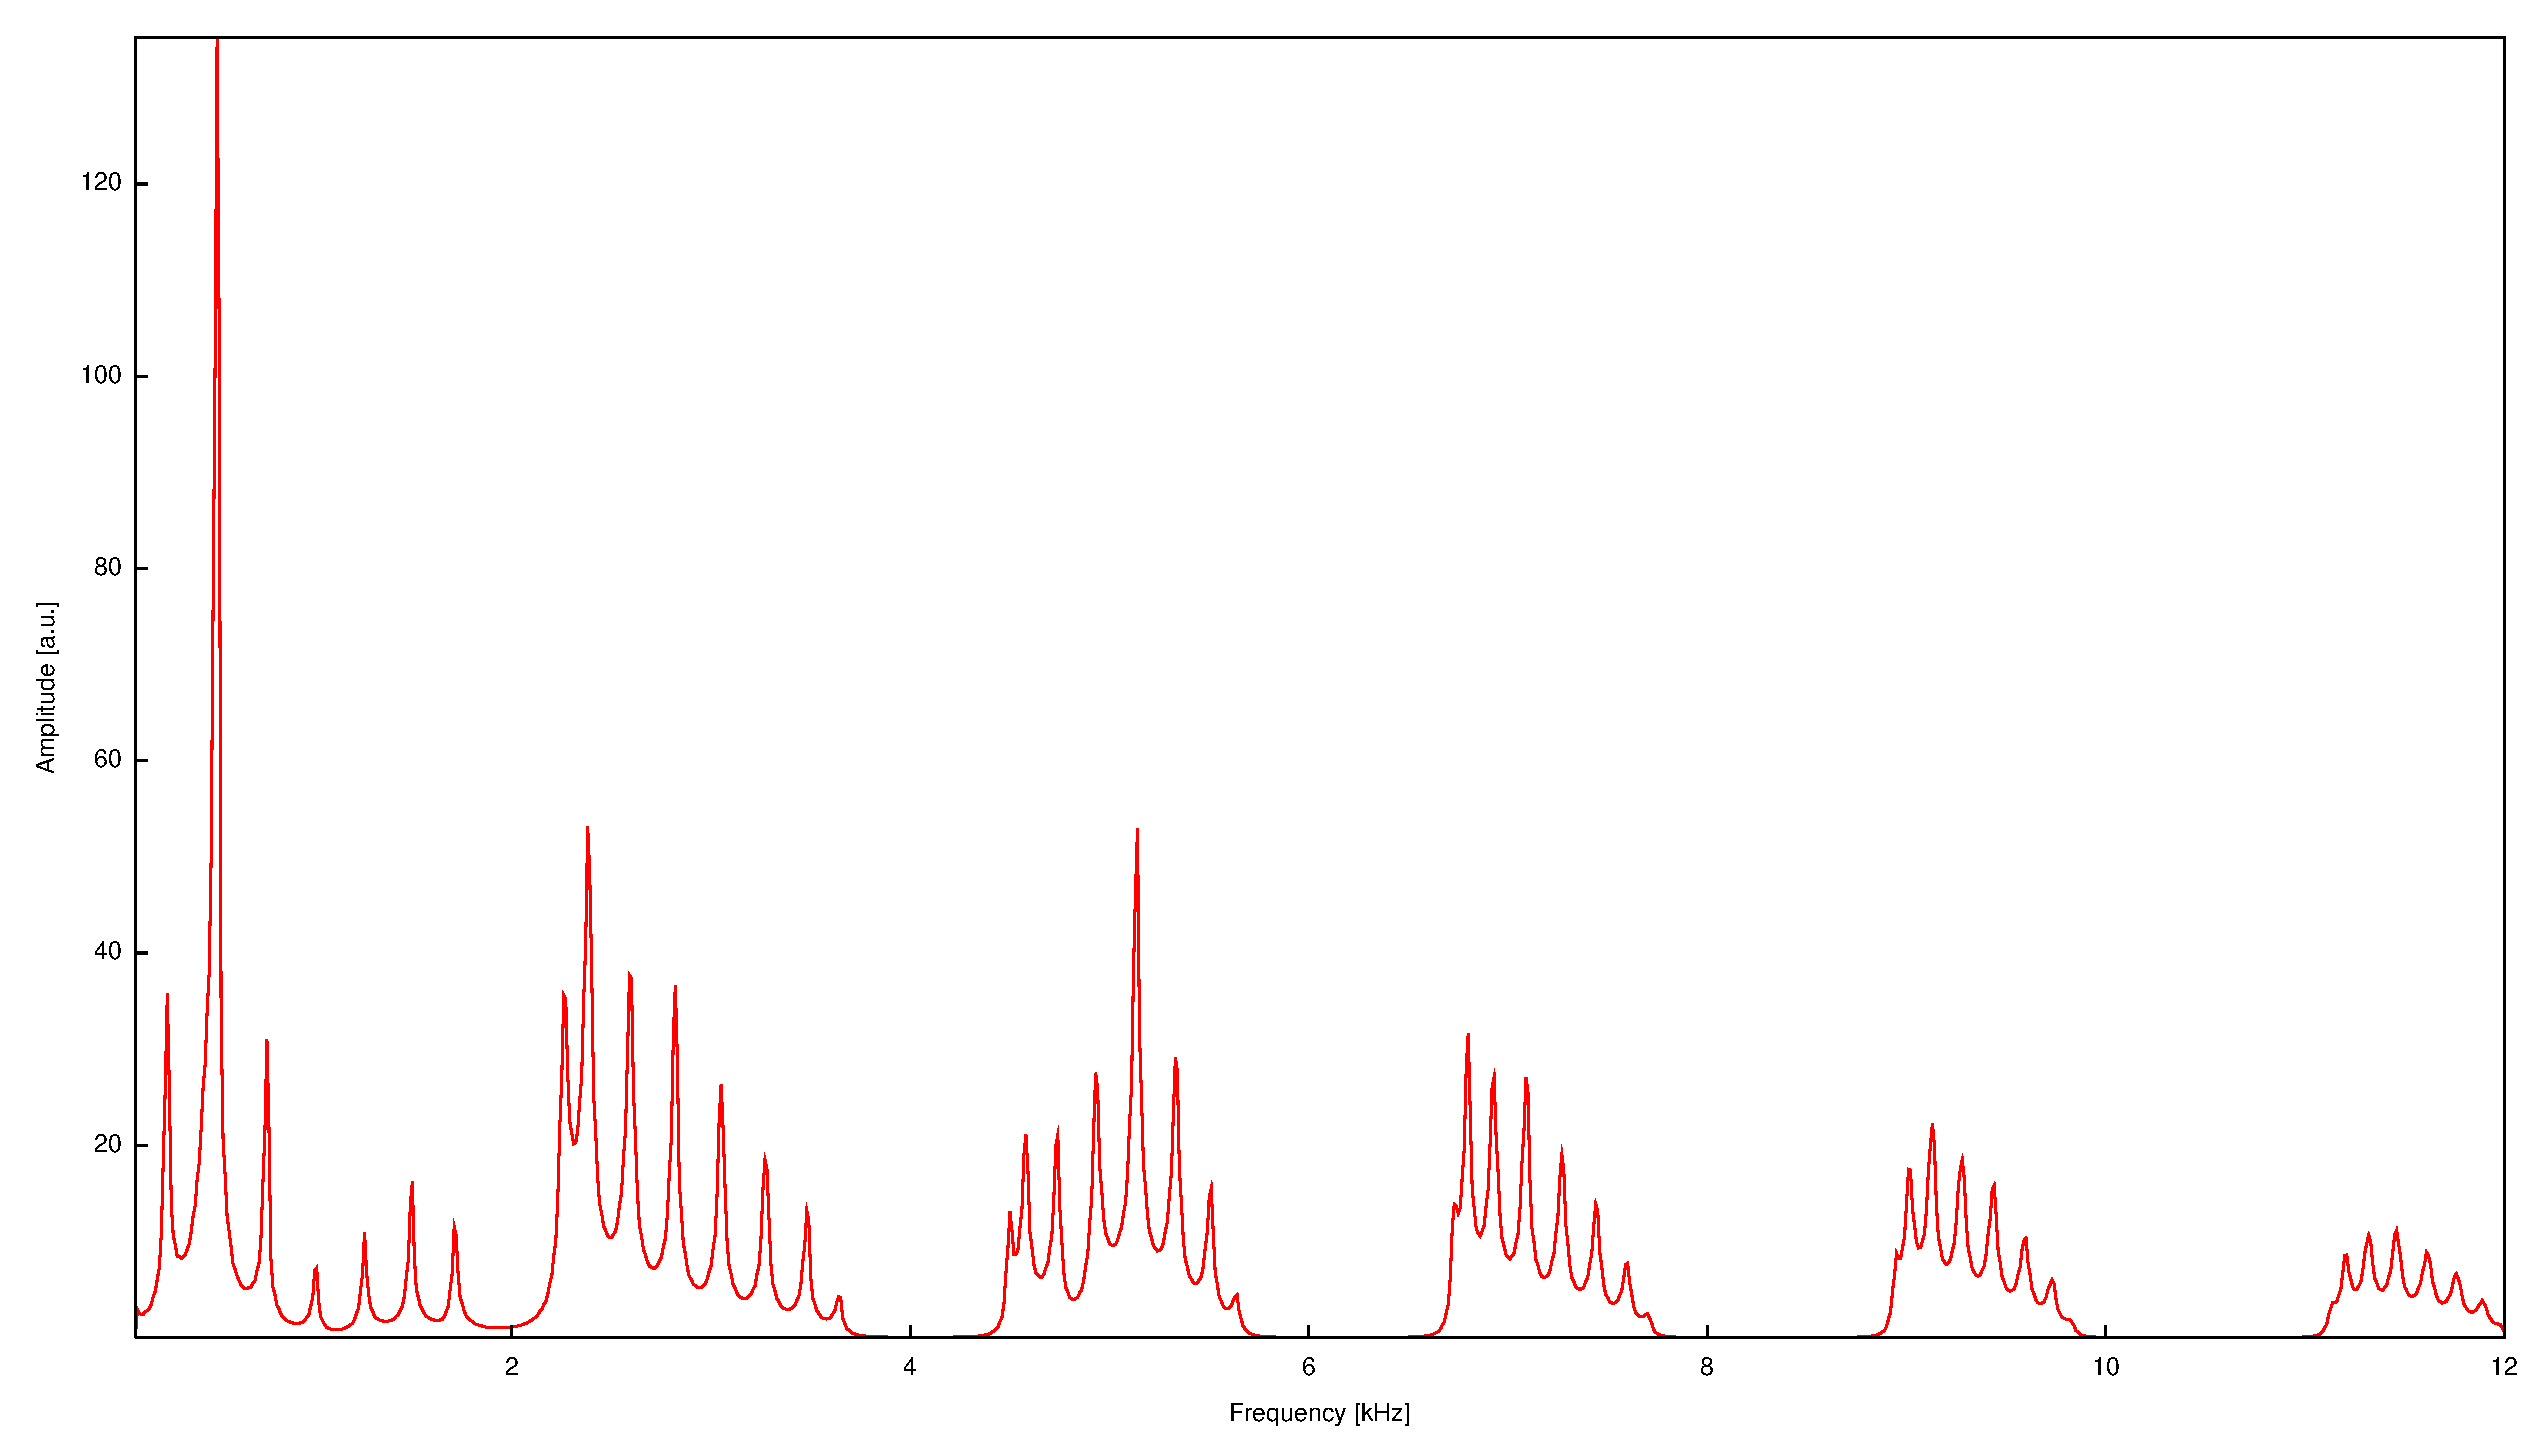
\includegraphics[width=\linewidth-60pt,height=\textheight-60pt,keepaspectratio]{FP-V23data/4.5_600mm_16mm.eps}
\caption{Spektrum von acht über $\SI{16}{\milli\meter}$-Irisse gekoppelten $\SI{75}{\milli\meter}$-Röhren}
\label{fig:8_75_16}
\end{figure}
\subsection{Atom-Molekül-Kette und Fehlstellen}
In Abbildung \ref{fig:50mm} ist das Spektrum einer $\SI{50}{\milli\meter}$-Röhre von $\SI{100}{\hertz}$ bis $\SI{22000}{\hertz}$ zu sehen. Bis $f\approx\SI{15000}{\hertz}$
sind die Peaks äquidistante longitudinale Moden. Für höhere Frequenzen sind die Abstände nicht mehr gleichmäßig und die Amplituden der Peaks wesentlich geringer. Sie beschreiben die transversalen Moden der Schallwelle in der Röhre.\\
In Abbildung \ref{fig:75mm} ist dasselbe Spektrum für eine $\SI{75}{\milli\meter}$-Röhre aufgenommen. Auch hier sind die longitudinalen Moden durch äquidistante Peaks bis etwa $\SI{15000}{\hertz}$ zu erkennen.\\
In Abbildung \ref{fig:50_10_50} ist das Spektrum von $\SI{100}{\hertz}$ bis $\SI{22000}{\hertz}$ einer Einheitszelle bestehend aus zwei über eine $\SI{10}{\milli\meter}$-Iris gekoppelten $\SI{50}{\milli\meter}$-Röhren zu sehen. Dieselbe Messung für eine $\SI{16}{\milli\meter}$-Kopplung ist in Abbildung \ref{fig:50_16_50} zu sehen. Es zeigt sich, dass die Breite der Bänder bei größerer Kopplung steigt während die Höhe der Peaks abnimmt. Auch ist bei größerem Innendurchmesser der Iris ein stärkerer Untergrund zu beobachten\\
%4.9?
In Abbildung \ref{fig:12_50_13_16} ist das Spektrum einer Folge von zwölf $\SI{50}{\milli\meter}$-Röhren, die abwechselnd über $\SI{13}{\milli\meter}$- und über $\SI{16}{\milli\meter}$-Irisse gekoppelt sind. Der Vergleich mit Abbildung \ref{fig:12_50_16} zeigt, dass sich bei alternierender Kopplung innerhalb der Bänder eine Substruktur bildet, die Anzahl der Peaks jedoch konstant bleibt.

\begin{figure}
\centering
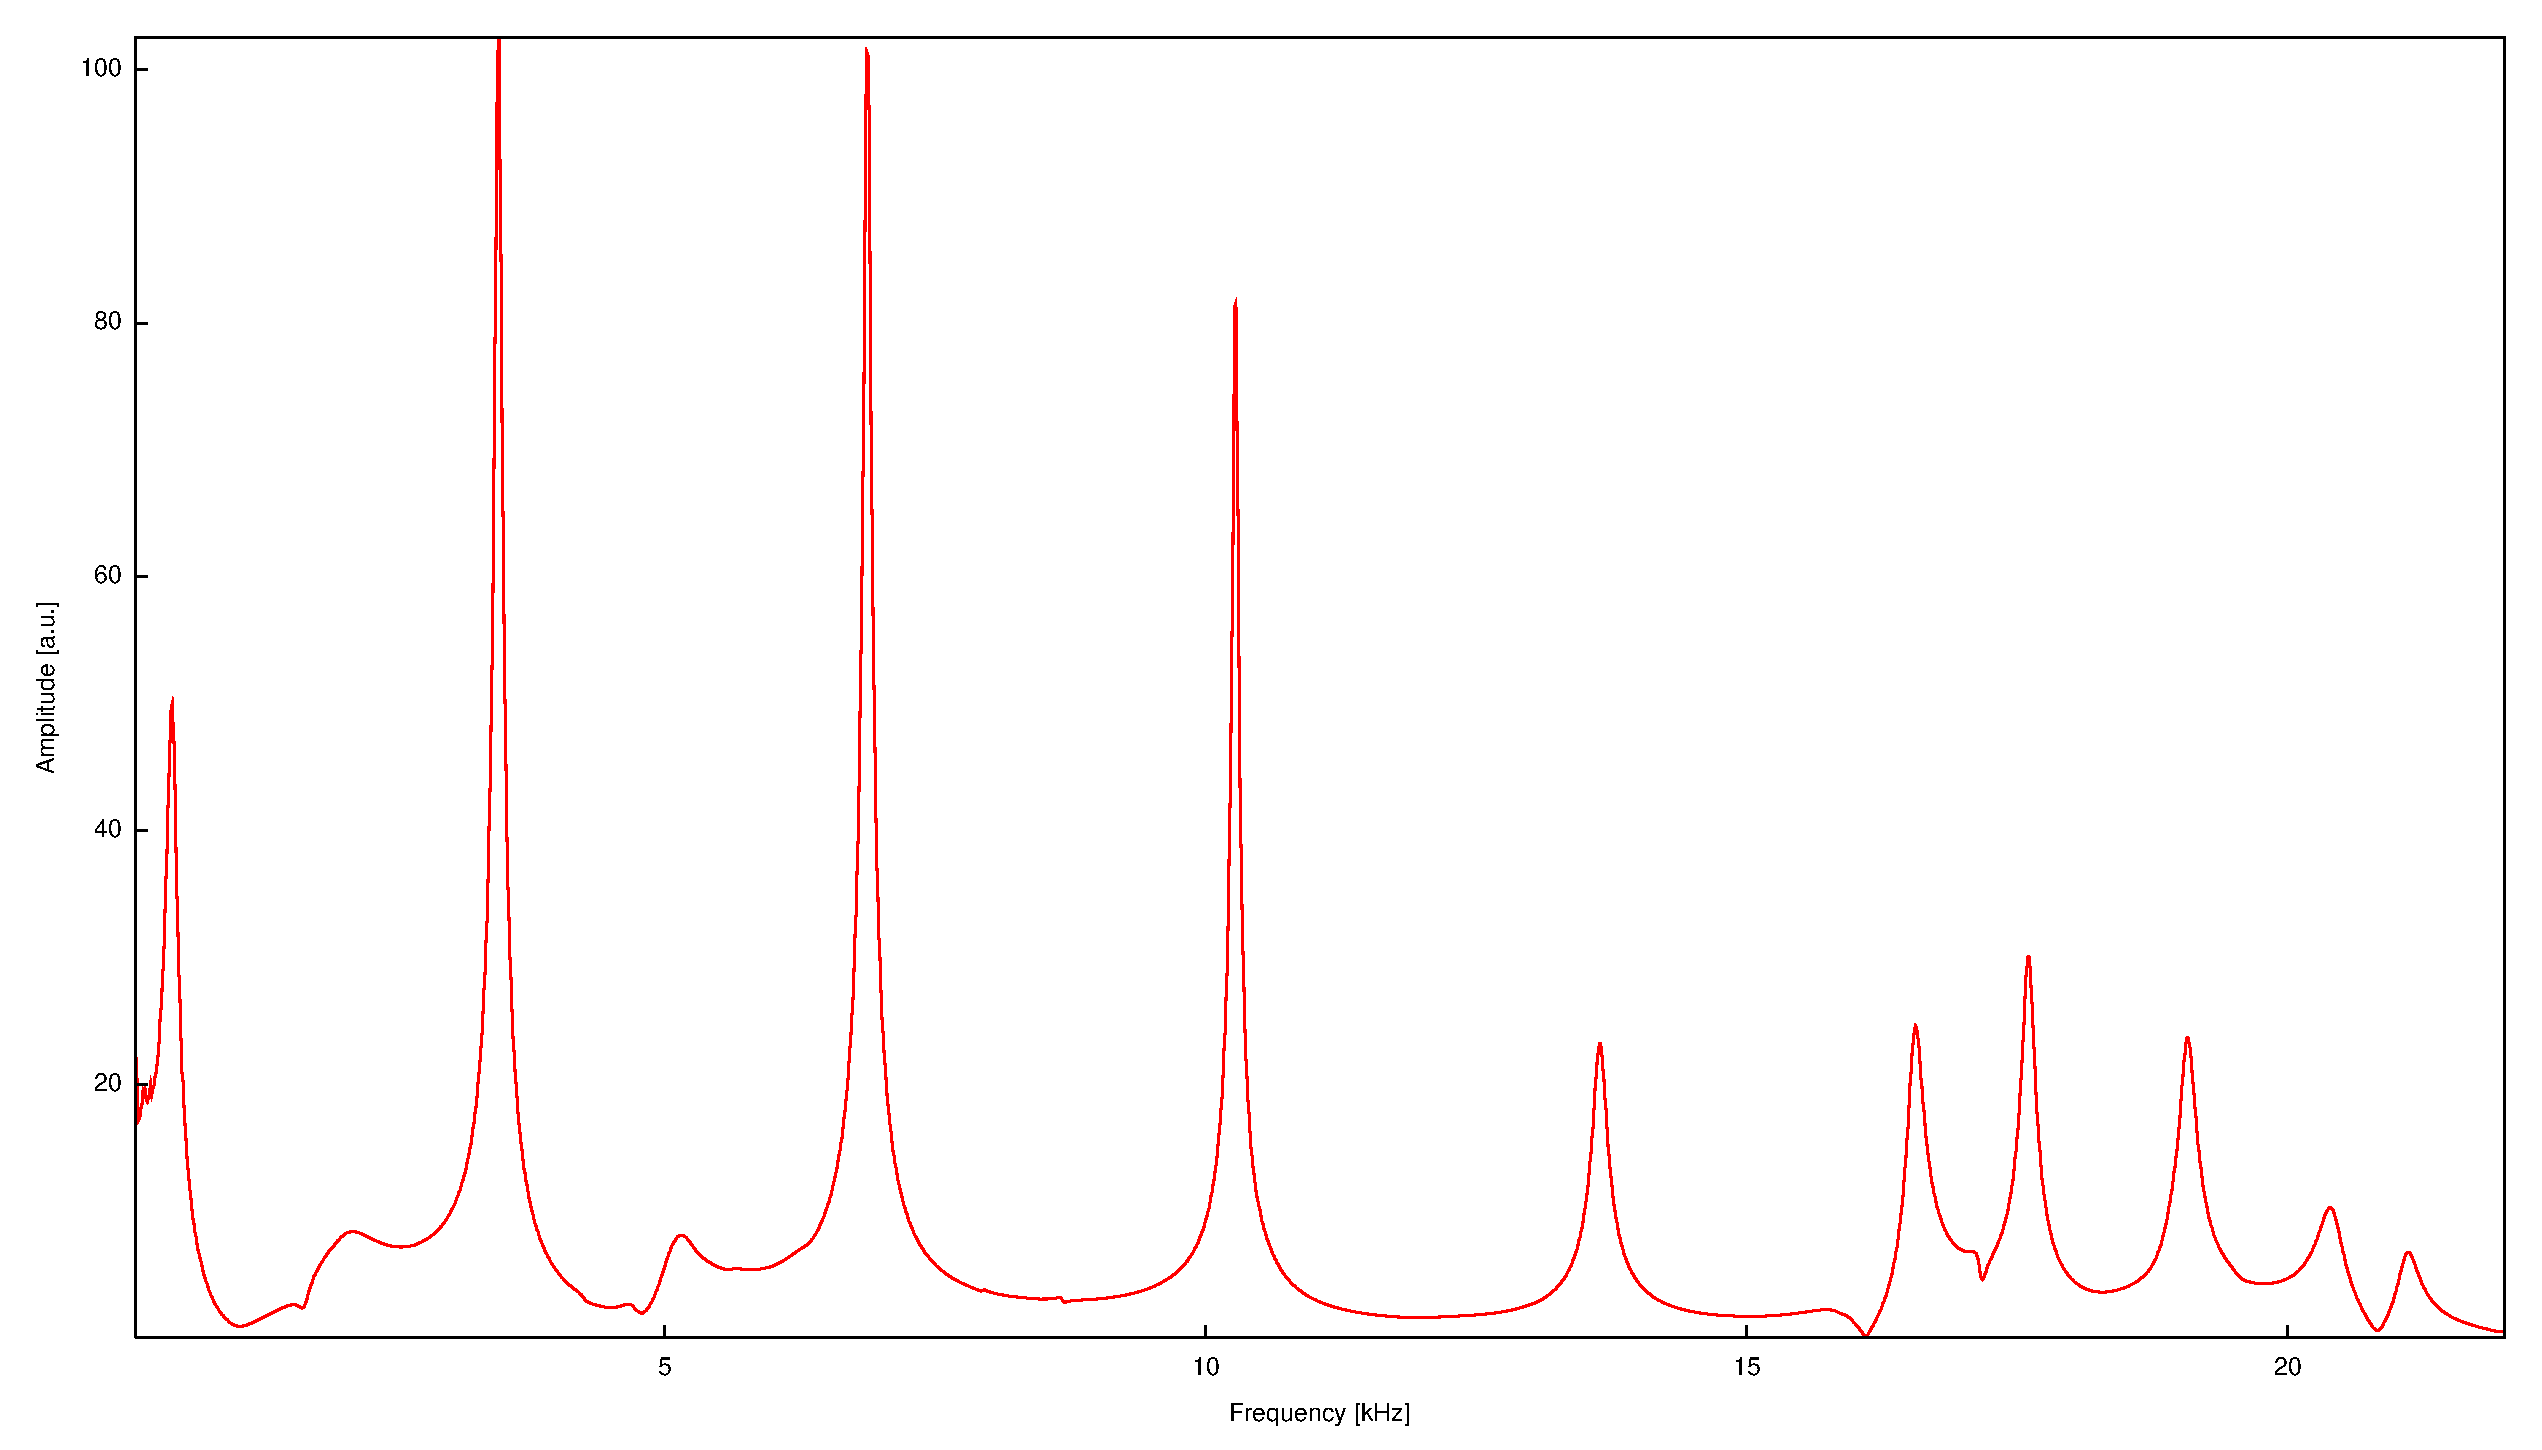
\includegraphics[width=\linewidth-60pt,height=\textheight-60pt,keepaspectratio]{FP-V23data/4.6_50mm.eps}
\caption{Spektrum von einer $\SI{75}{\milli\meter}$-Röhre}
\label{fig:50mm}
\end{figure}
\begin{figure}
\centering
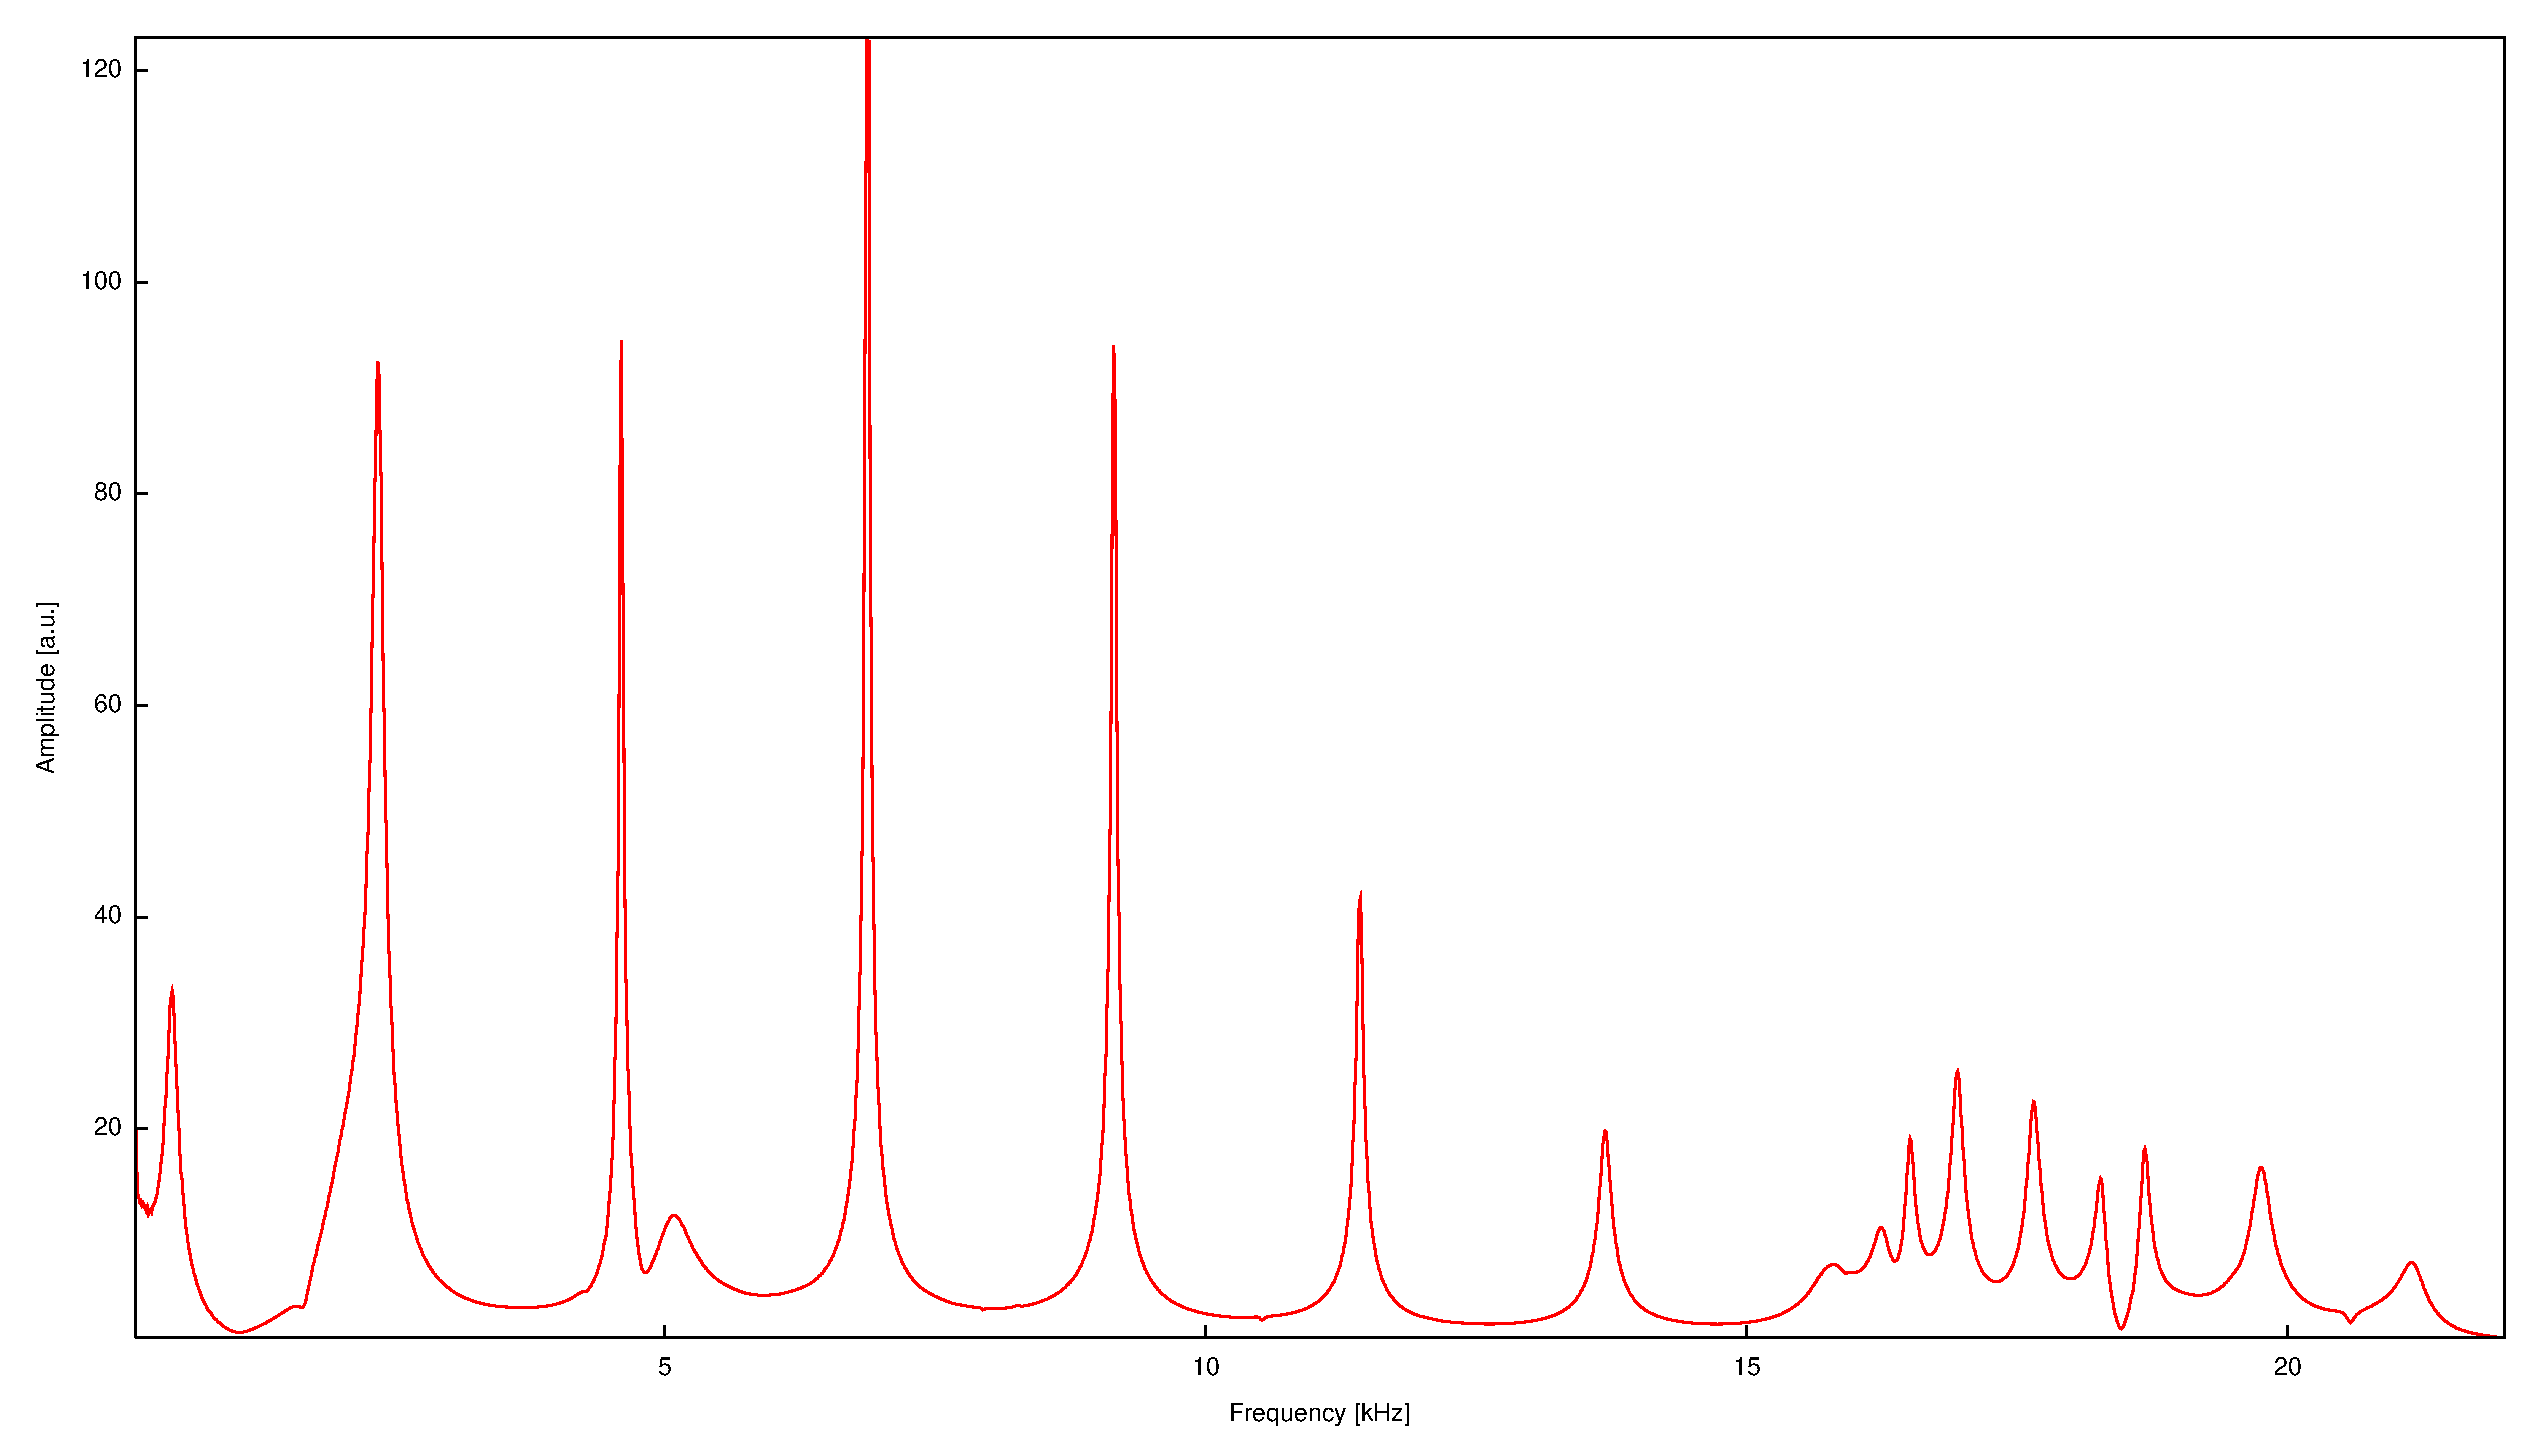
\includegraphics[width=\linewidth-60pt,height=\textheight-60pt,keepaspectratio]{FP-V23data/4.7_75mm.eps}
\caption{Spektrum von einer $\SI{75}{\milli\meter}$-Röhre}
\label{fig:75mm}
\end{figure}
\begin{figure}
\centering
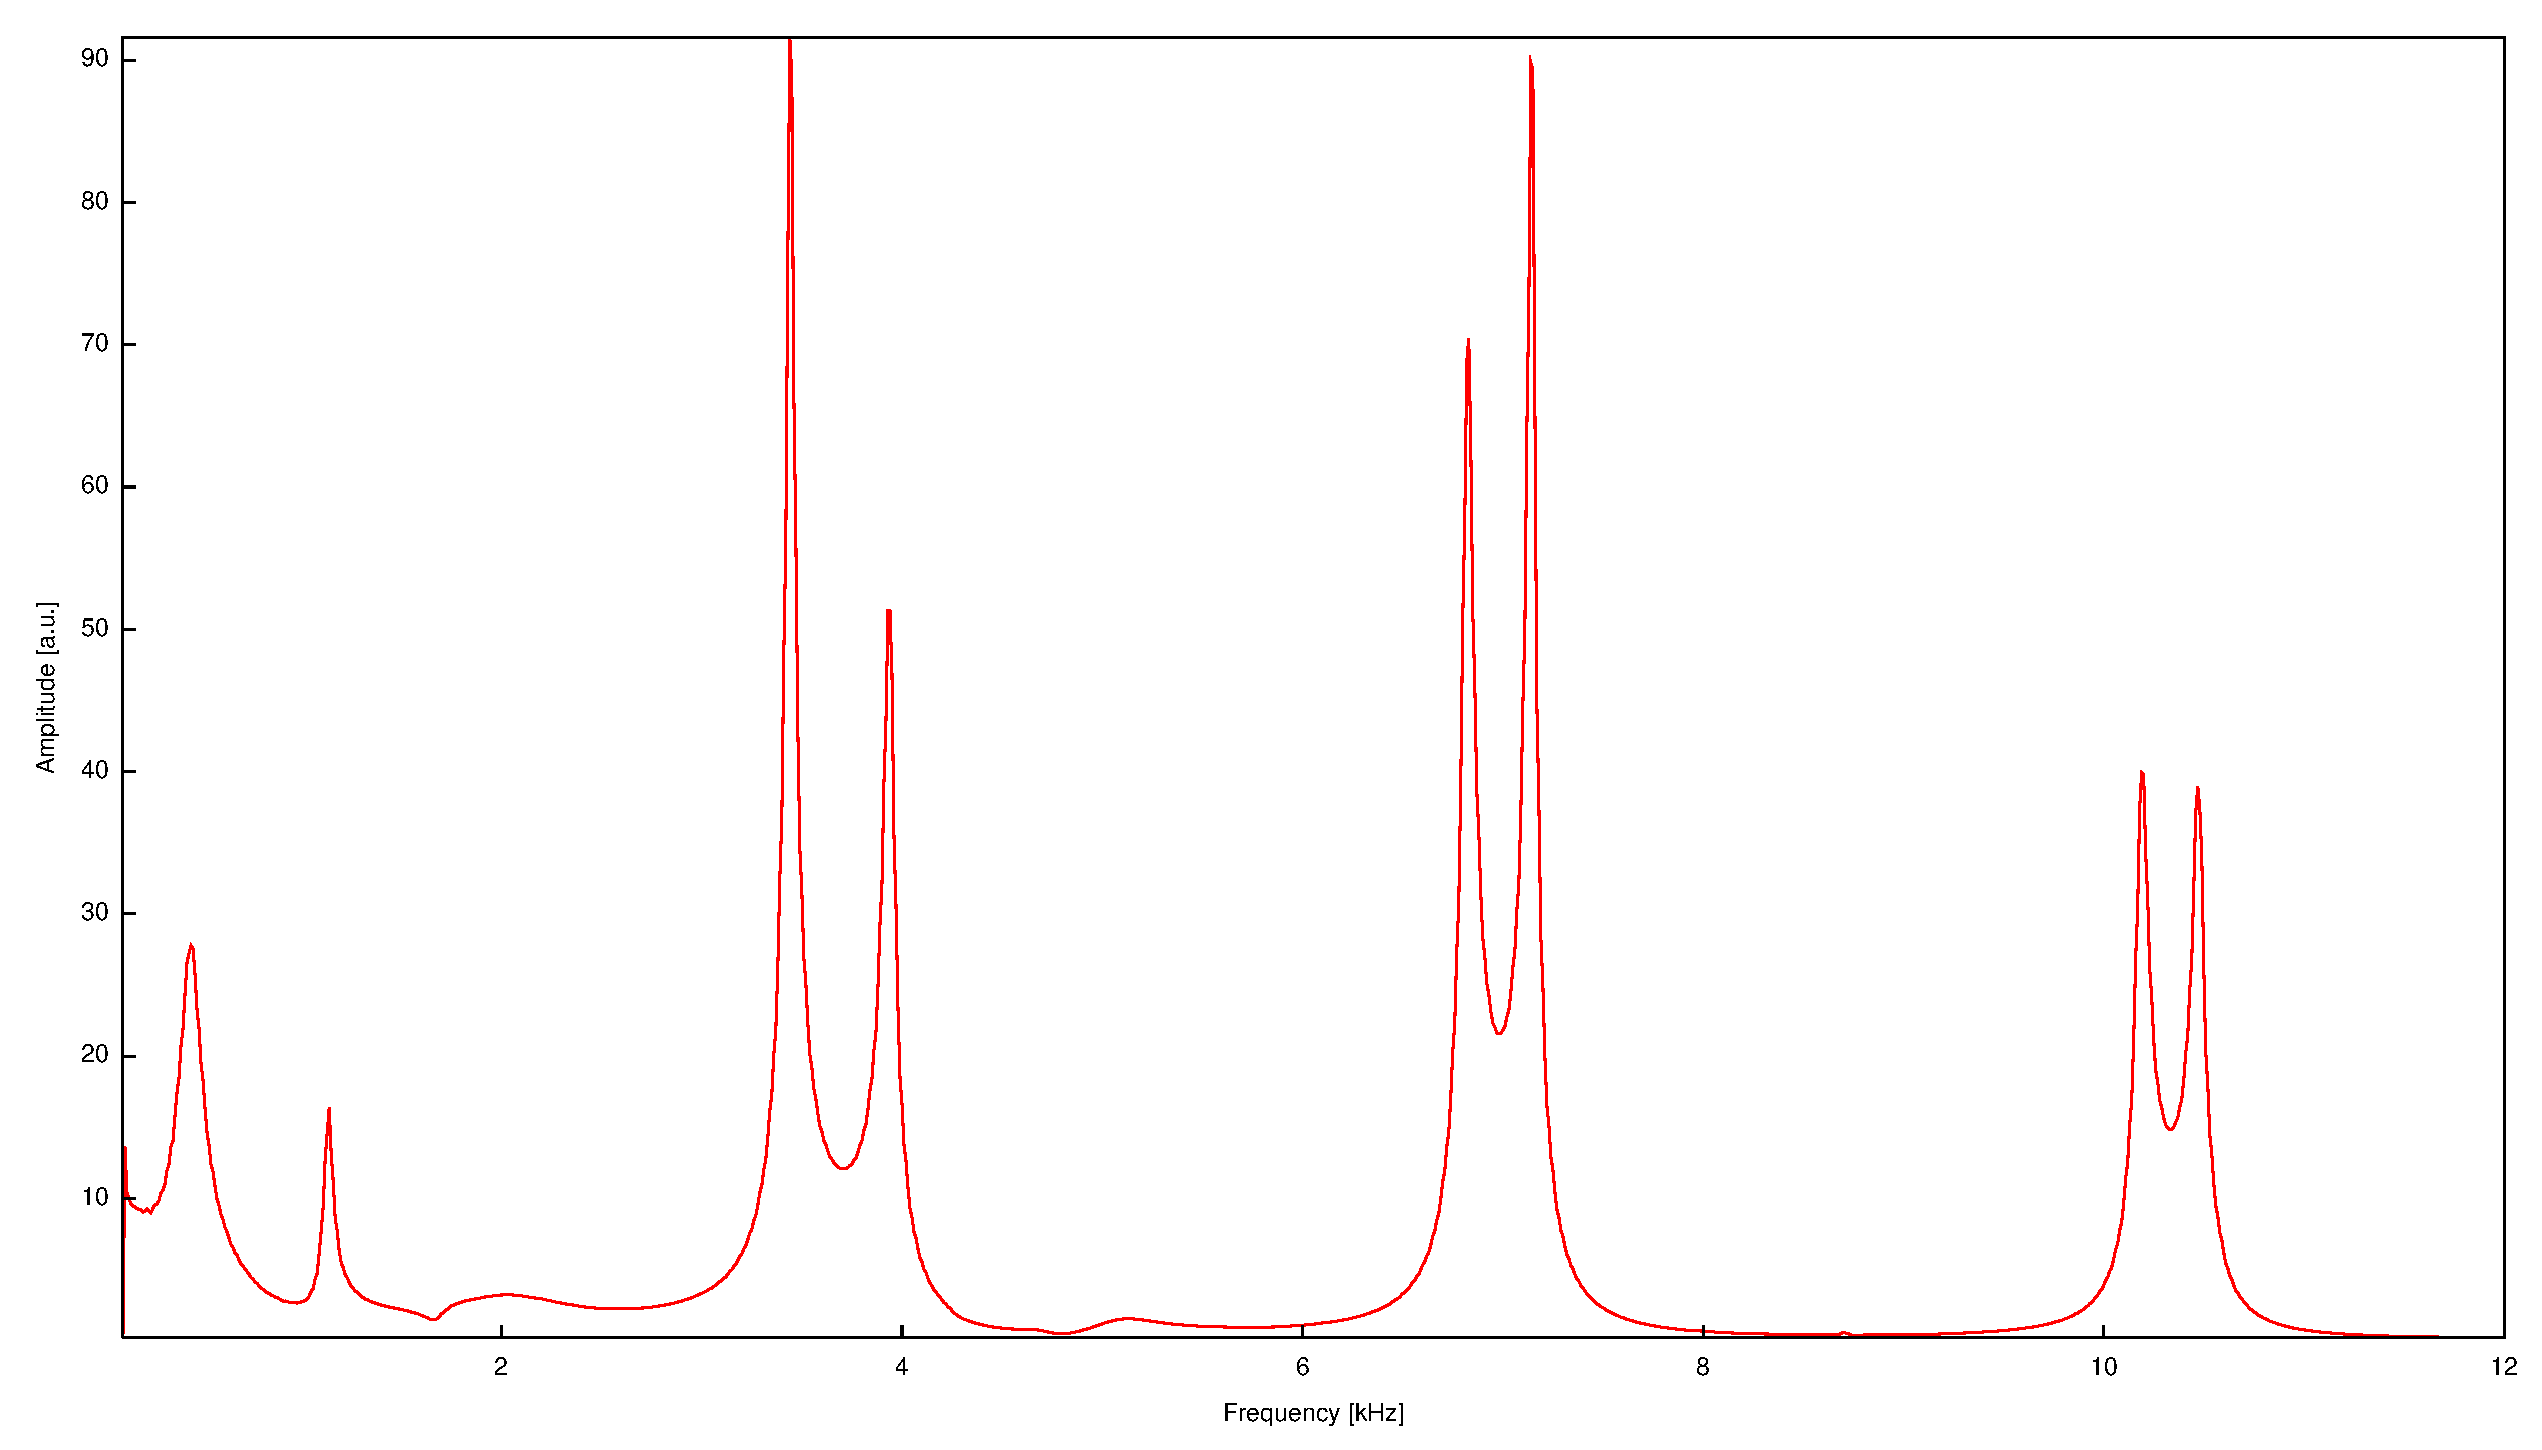
\includegraphics[width=\linewidth-60pt,height=\textheight-60pt,keepaspectratio]{FP-V23data/4.8_100mm_10mm.eps}
\caption{Spektrum von einer Einheitszelle bestehend aus zwei über $\SI{10}{\milli\meter}$-Irisse gekoppelten $\SI{50}{\milli\meter}$-Röhren}
\label{fig:50_10_50}
\end{figure}
\begin{figure}
\centering
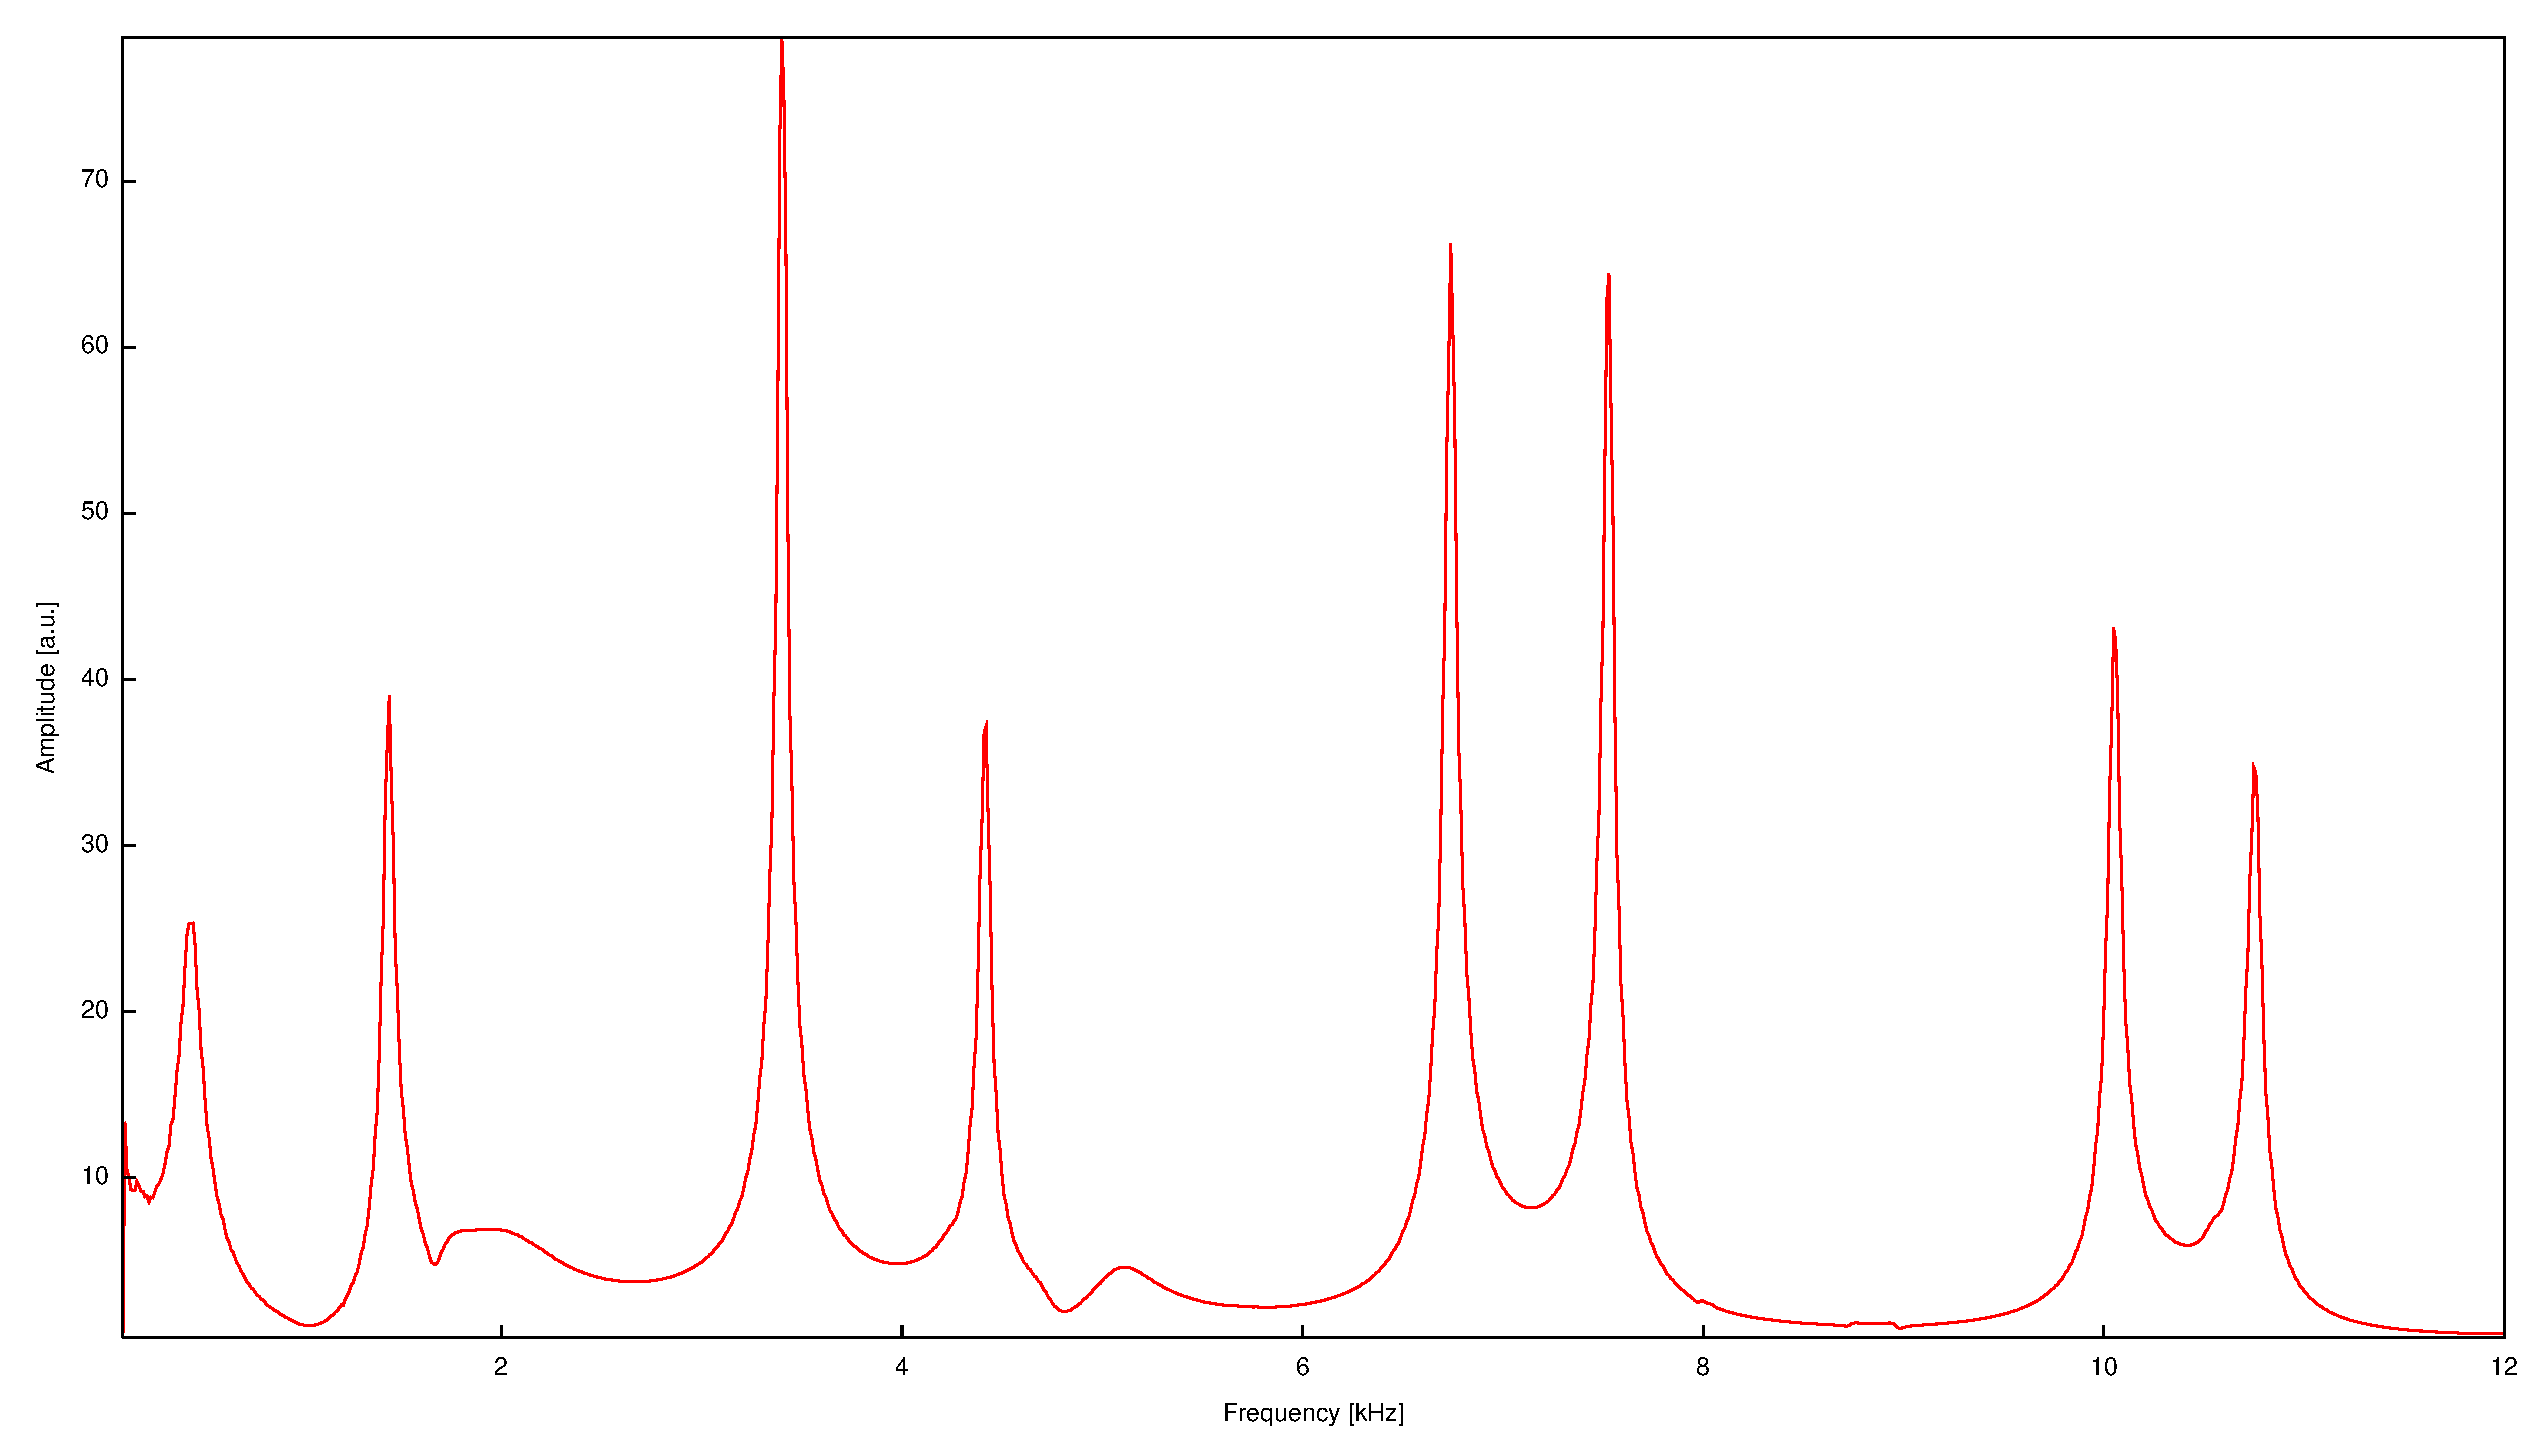
\includegraphics[width=\linewidth-60pt,height=\textheight-60pt,keepaspectratio]{FP-V23data/4.8_100mm_16mm.eps}
\caption{Spektrum von einer Einheitszelle bestehend aus zwei über $\SI{16}{\milli\meter}$-Irisse gekoppelten $\SI{50}{\milli\meter}$-Röhren}
\label{fig:50_16_50}
\end{figure}
\begin{figure}
\centering
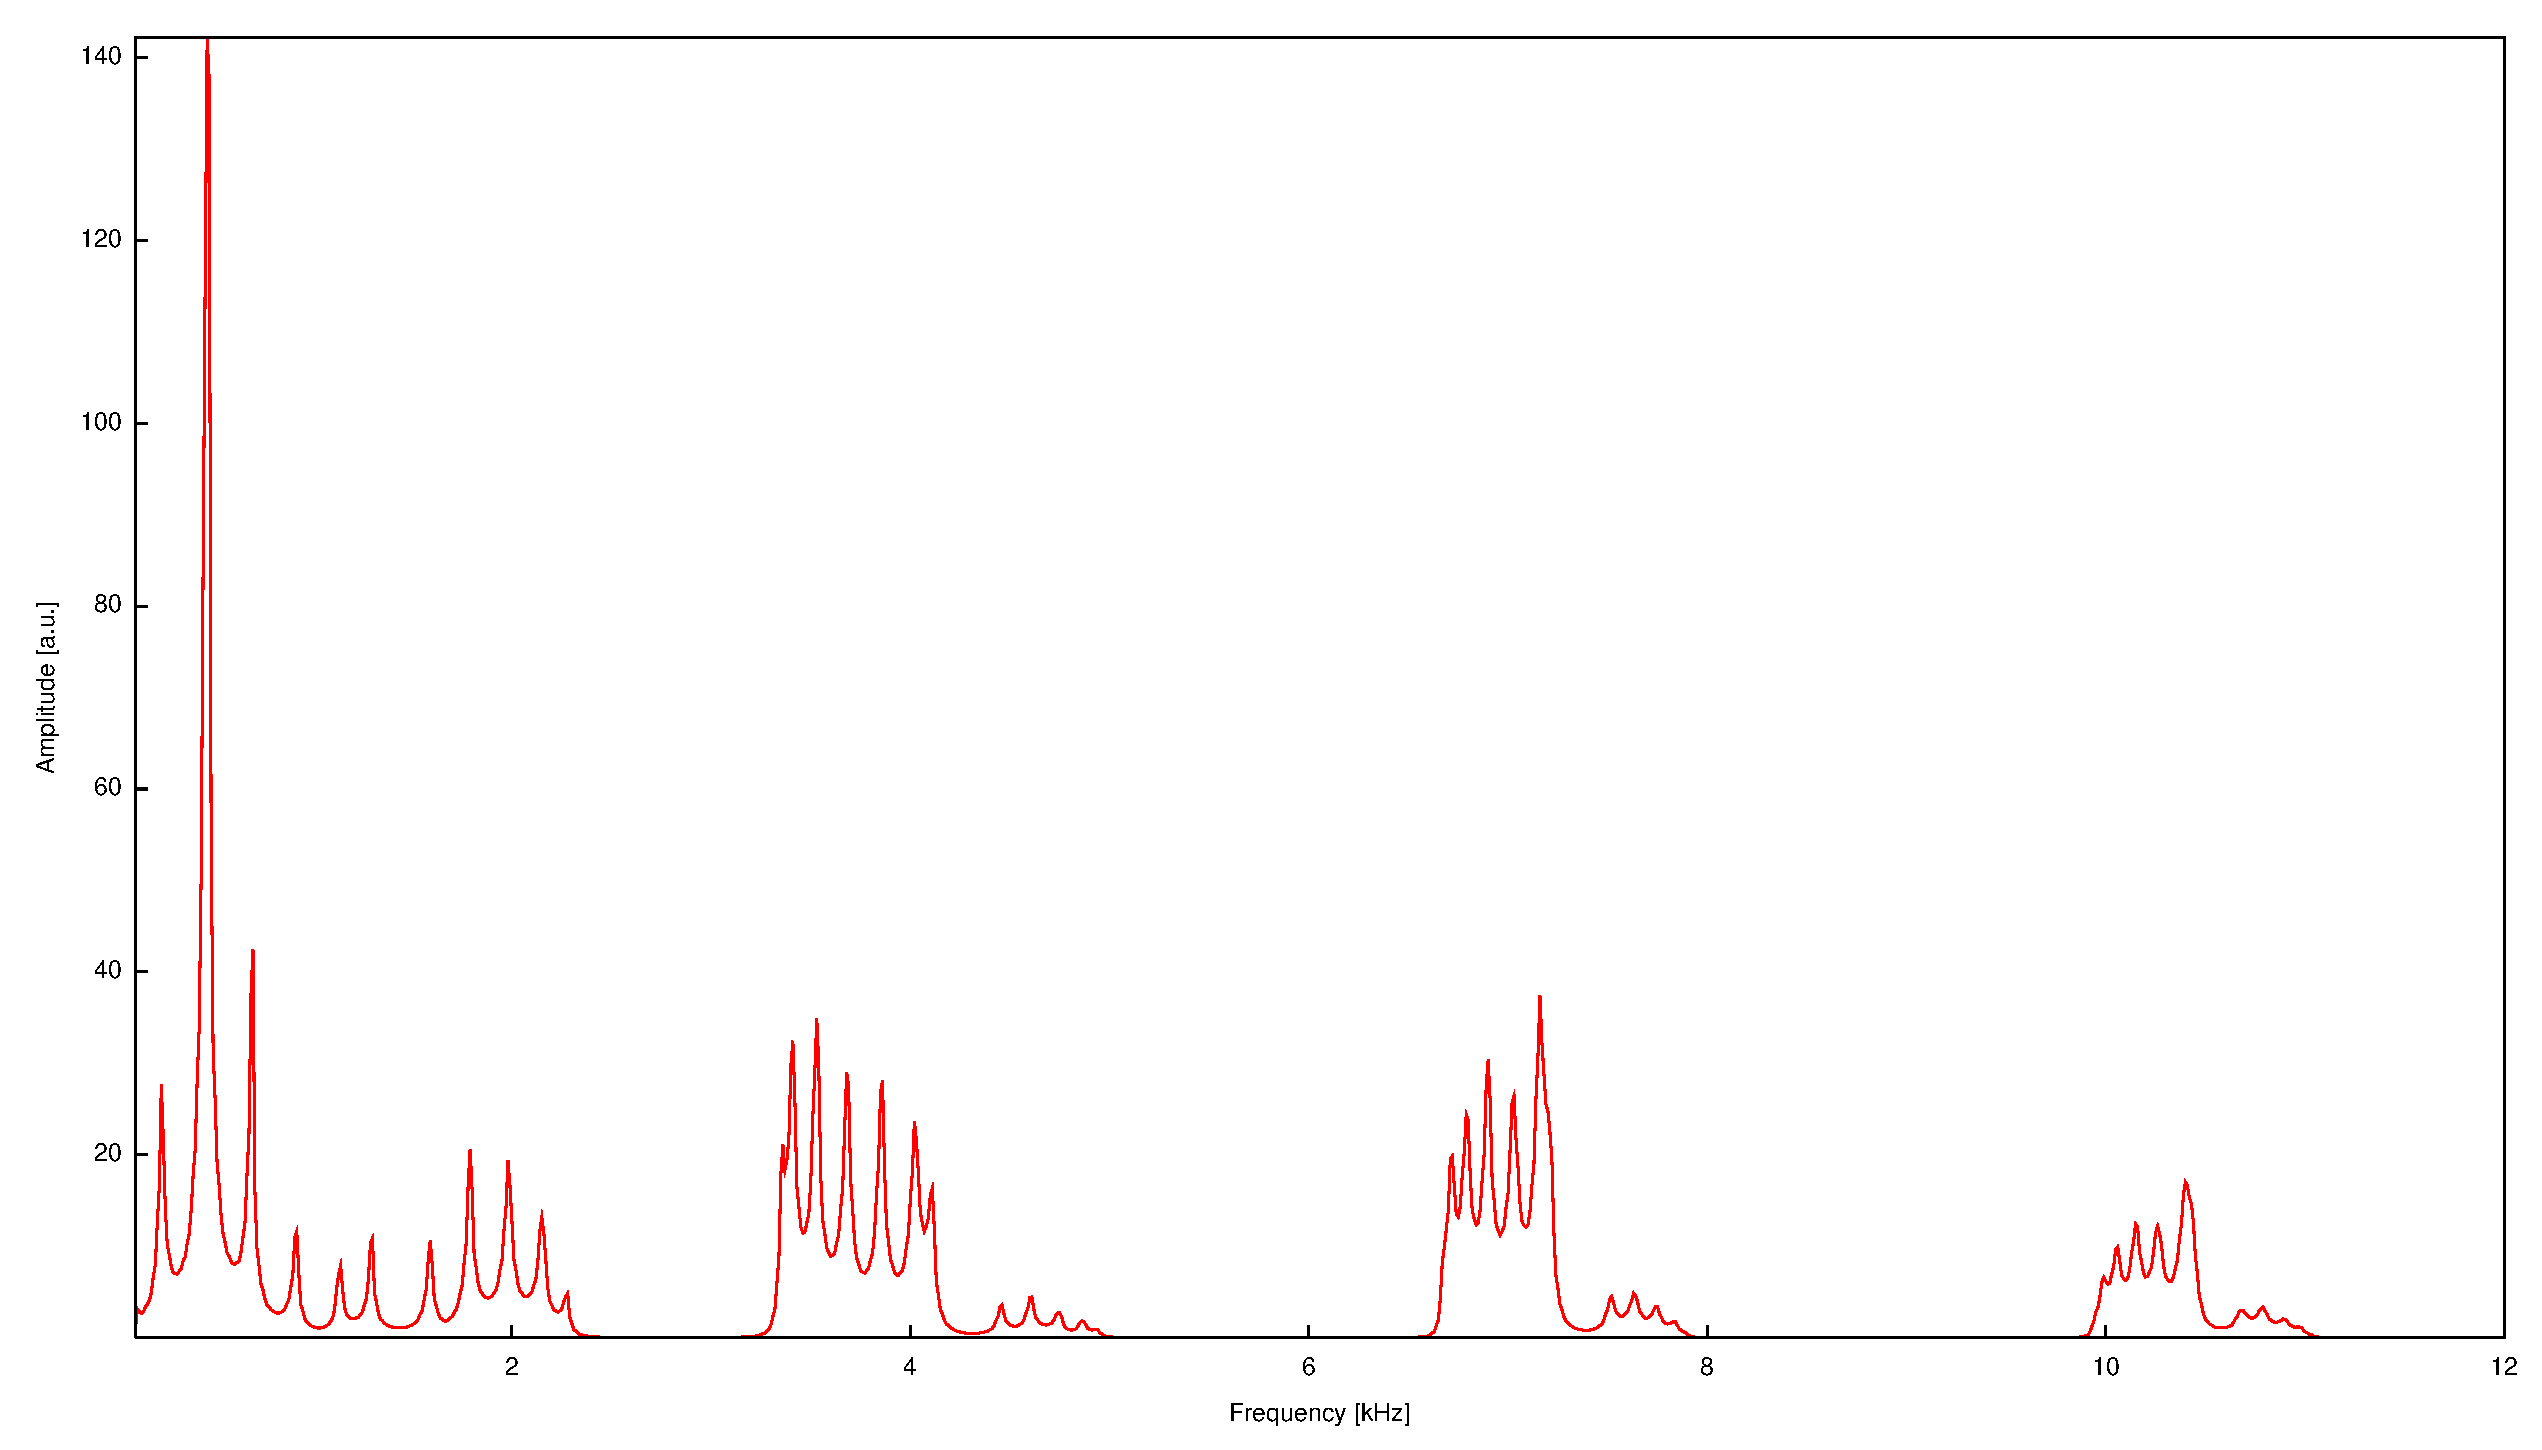
\includegraphics[width=\linewidth-60pt,height=\textheight-60pt,keepaspectratio]{FP-V23data/4.10_600mm_13_16mm.eps}
\caption{Spektrum von zwölf abwechselnd über $13$- und $\SI{16}{\milli\meter}$-Irisse gekoppelten $\SI{50}{\milli\meter}$-Röhren}
\label{fig:12_50_13_16}
\end{figure}


%◘♦☻♥◘○☺♠◘
